\documentclass[]{tufte-book}

% ams
\usepackage{amssymb,amsmath}

\usepackage{ifxetex,ifluatex}
\usepackage{fixltx2e} % provides \textsubscript
\ifnum 0\ifxetex 1\fi\ifluatex 1\fi=0 % if pdftex
  \usepackage[T1]{fontenc}
  \usepackage[utf8]{inputenc}
\else % if luatex or xelatex
  \makeatletter
  \@ifpackageloaded{fontspec}{}{\usepackage{fontspec}}
  \makeatother
  \defaultfontfeatures{Ligatures=TeX,Scale=MatchLowercase}
  \makeatletter
  \@ifpackageloaded{soul}{
     \renewcommand\allcapsspacing[1]{{\addfontfeature{LetterSpace=15}#1}}
     \renewcommand\smallcapsspacing[1]{{\addfontfeature{LetterSpace=10}#1}}
   }{}
  \makeatother
\fi

% graphix
\usepackage{graphicx}
\setkeys{Gin}{width=\linewidth,totalheight=\textheight,keepaspectratio}

% booktabs
\usepackage{booktabs}

% url
\usepackage{url}

% hyperref
\usepackage{hyperref}

% units.
\usepackage{units}


\setcounter{secnumdepth}{2}

% citations

% pandoc syntax highlighting
\usepackage{color}
\usepackage{fancyvrb}
\newcommand{\VerbBar}{|}
\newcommand{\VERB}{\Verb[commandchars=\\\{\}]}
\DefineVerbatimEnvironment{Highlighting}{Verbatim}{commandchars=\\\{\}}
% Add ',fontsize=\small' for more characters per line
\newenvironment{Shaded}{}{}
\newcommand{\KeywordTok}[1]{\textcolor[rgb]{0.00,0.44,0.13}{\textbf{#1}}}
\newcommand{\DataTypeTok}[1]{\textcolor[rgb]{0.56,0.13,0.00}{#1}}
\newcommand{\DecValTok}[1]{\textcolor[rgb]{0.25,0.63,0.44}{#1}}
\newcommand{\BaseNTok}[1]{\textcolor[rgb]{0.25,0.63,0.44}{#1}}
\newcommand{\FloatTok}[1]{\textcolor[rgb]{0.25,0.63,0.44}{#1}}
\newcommand{\ConstantTok}[1]{\textcolor[rgb]{0.53,0.00,0.00}{#1}}
\newcommand{\CharTok}[1]{\textcolor[rgb]{0.25,0.44,0.63}{#1}}
\newcommand{\SpecialCharTok}[1]{\textcolor[rgb]{0.25,0.44,0.63}{#1}}
\newcommand{\StringTok}[1]{\textcolor[rgb]{0.25,0.44,0.63}{#1}}
\newcommand{\VerbatimStringTok}[1]{\textcolor[rgb]{0.25,0.44,0.63}{#1}}
\newcommand{\SpecialStringTok}[1]{\textcolor[rgb]{0.73,0.40,0.53}{#1}}
\newcommand{\ImportTok}[1]{#1}
\newcommand{\CommentTok}[1]{\textcolor[rgb]{0.38,0.63,0.69}{\textit{#1}}}
\newcommand{\DocumentationTok}[1]{\textcolor[rgb]{0.73,0.13,0.13}{\textit{#1}}}
\newcommand{\AnnotationTok}[1]{\textcolor[rgb]{0.38,0.63,0.69}{\textbf{\textit{#1}}}}
\newcommand{\CommentVarTok}[1]{\textcolor[rgb]{0.38,0.63,0.69}{\textbf{\textit{#1}}}}
\newcommand{\OtherTok}[1]{\textcolor[rgb]{0.00,0.44,0.13}{#1}}
\newcommand{\FunctionTok}[1]{\textcolor[rgb]{0.02,0.16,0.49}{#1}}
\newcommand{\VariableTok}[1]{\textcolor[rgb]{0.10,0.09,0.49}{#1}}
\newcommand{\ControlFlowTok}[1]{\textcolor[rgb]{0.00,0.44,0.13}{\textbf{#1}}}
\newcommand{\OperatorTok}[1]{\textcolor[rgb]{0.40,0.40,0.40}{#1}}
\newcommand{\BuiltInTok}[1]{#1}
\newcommand{\ExtensionTok}[1]{#1}
\newcommand{\PreprocessorTok}[1]{\textcolor[rgb]{0.74,0.48,0.00}{#1}}
\newcommand{\AttributeTok}[1]{\textcolor[rgb]{0.49,0.56,0.16}{#1}}
\newcommand{\RegionMarkerTok}[1]{#1}
\newcommand{\InformationTok}[1]{\textcolor[rgb]{0.38,0.63,0.69}{\textbf{\textit{#1}}}}
\newcommand{\WarningTok}[1]{\textcolor[rgb]{0.38,0.63,0.69}{\textbf{\textit{#1}}}}
\newcommand{\AlertTok}[1]{\textcolor[rgb]{1.00,0.00,0.00}{\textbf{#1}}}
\newcommand{\ErrorTok}[1]{\textcolor[rgb]{1.00,0.00,0.00}{\textbf{#1}}}
\newcommand{\NormalTok}[1]{#1}

% longtable
\usepackage{longtable,booktabs}

% multiplecol
\usepackage{multicol}

% strikeout
\usepackage[normalem]{ulem}

% morefloats
\usepackage{morefloats}


% tightlist macro required by pandoc >= 1.14
\providecommand{\tightlist}{%
  \setlength{\itemsep}{0pt}\setlength{\parskip}{0pt}}

% title / author / date
\title{R for the Health, Behavioral, and Social Sciences}
\author{Tyson S. Barrett}
\date{2017-07-03}


\usepackage{amsthm}
\newtheorem{theorem}{Theorem}[chapter]
\newtheorem{lemma}{Lemma}[chapter]
\theoremstyle{definition}
\newtheorem{definition}{Definition}[chapter]
\newtheorem{corollary}{Corollary}[chapter]
\newtheorem{proposition}{Proposition}[chapter]
\theoremstyle{definition}
\newtheorem{example}{Example}[chapter]
\theoremstyle{remark}
\newtheorem*{remark}{Remark}
\begin{document}

\maketitle



{
\setcounter{tocdepth}{1}
\tableofcontents
}

\chapter*{Preface}\label{preface}
\addcontentsline{toc}{chapter}{Preface}

\begin{quote}
``Somewhere, something incredible is waiting to be known.''

--- Carl Sagan
\end{quote}

\texttt{R} is made for scientists pursuing discoveries; discoveries that
cannot be solved with human intuition alone. \texttt{R} is capable of
data analysis in nearly any form. It is an open-source project meaning
it can be extended and fixed by countless individuals around the world.
It is almost always on the cutting edge of new techniques and methods.
Yet, many are hesitant to learn to use it.

This is probably due to the high learning curve. Although challenging,
with a little guidance, the journey in learning \texttt{R} programming
can be made much simpler. It is for this exact reason this book was
written.

Although there are many books and websites devoted to R, I've noticed
that a simple introduction---without excessive information on things
that are unlikely to be used---was lacking, particularly for the health,
behavioral, and social sciences. This book began as I, working as a data
science and statistical consultant, was trying to help my clientele with
quantitative research across these fields. Three main reasons kept me
repeatedly recommending my clients to use \texttt{R}: the replicability
of the \texttt{R} centered workflow, the powerful and beautiful plotting
capabilities, and the simple---yet extensive---data management/analysis
tools.

This book is for beginners in \texttt{R}; especially those in health,
behavioral and social sciences. I picked those fields specifically
because much of their research overlaps in data types, methodologies
employed, and in hypotheses tested. Both exploratory and confirmatory
methods will be highlighted given their importance in these fields,
among many others.

I'll introduce you to many ways in which \texttt{R} can be used in your
work. You'll find that it can help in all facets of your data analysis
and communication, while improving your replicability. In the long run,
taking some time to learn a new tool will save you time, energy, and
probably most importantly, frustration. When a researcher is frustrated,
it becomes so easy to overlook important features.

We will quickly, and succinctly, introduce the newest, easiest, and most
understandable ways of working with your data. To do this, we will have
three main parts: 1) working with and simple analyses of your data, 2)
modeling your data, and 3) more advanced techniques to help your
workflow.

\section*{Part I}\label{part-i}
\addcontentsline{toc}{section}{Part I}

\begin{enumerate}
\def\labelenumi{\arabic{enumi}.}
\tightlist
\item
  Chapter 1: The basics of the language
\item
  Chapter 2: Working with and Cleaning Your Data
\item
  Chapter 3: Understanding your data (summary statistics, ggplot2)
\end{enumerate}

\section*{Part II}\label{part-ii}
\addcontentsline{toc}{section}{Part II}

\begin{enumerate}
\def\labelenumi{\arabic{enumi}.}
\setcounter{enumi}{3}
\tightlist
\item
  Chapter 4: Basic Statistical Analyses (ANOVA, Linear Regression)
\item
  Chapter 5: Generalized Linear Models
\item
  Chapter 6: Mulilevel Modeling
\item
  Chapter 7: Other Modeling Techniques
\end{enumerate}

\section*{Part III}\label{part-iii}
\addcontentsline{toc}{section}{Part III}

\begin{enumerate}
\def\labelenumi{\arabic{enumi}.}
\setcounter{enumi}{7}
\tightlist
\item
  Chapter 8: Advanced data manipulation
\item
  Chapter 9: Advanced plotting
\item
  Chapter 10: Where to go from here
\end{enumerate}

At the end of the book, you should be able to: 1) use \texttt{R} to
perform your data cleaning and data analyses and 2) understand online
helps (e.g. \url{www.stackoverflow.com}, \url{www.r-bloggers.com}) so
your potential in \texttt{R} becomes nearly limitless.

\section*{Download R and RStudio}\label{download-r-and-rstudio}
\addcontentsline{toc}{section}{Download R and RStudio}

To begin, you will need to download the \texttt{R} software
\href{https://www.r-project.org/}{www.r-project.org} and then the
RStudio software \href{https://www.rstudio.com/}{www.rstudio.com}.
\texttt{R} is the brains and \texttt{RStudio}\footnote{Get the free
  version of \texttt{Rstudio}. Believe me, it doesn't feel like it
  should be free software.} is an ``IDE'' (something that helps us work
with \texttt{R} much more easily).

Once both are installed (helps on installing the software can be found
on \href{https://www.rstudio.com/}{www.rstudio.com},
\url{www.r-bloggers.com}, and \url{www.statmethods.net}) you are good to
go. The remainder of the book will be about actually using it.

Enjoy!\footnote{Note that to return to Tyson's blog, you can click
  \href{https://tysonstanley.github.io}{here}}

\chapter*{Chapter 1: The Basics of the
Language}\label{chapter-1-the-basics-of-the-language}
\addcontentsline{toc}{chapter}{Chapter 1: The Basics of the Language}

\begin{quote}
``Success is neither magical nor mysterious. Success is the natural
consequence of consistently applying the basic fundamentals.''

--- Jim Rohn
\end{quote}

\texttt{R} is an open source statistical software made by statisticians.
This means it generally speaks the language of statistics. This is very
helpful when it comes running analyses but can be confusing when
starting to understand the code.

The best way to begin to learn it is by jumping right into it. This
chapter will provide the background and foundation to start using
\texttt{R} right away. This background revolves around data and
functions---two types of objects.

\section*{Objects}\label{objects}
\addcontentsline{toc}{section}{Objects}

\texttt{R} is built on a few different types of virtual objects. An
object, just like in the physical world, is something you can do things
with. In the real world, we have objects that we use regularly. For
example, we have chairs. Chairs are great for some things (sitting on,
sleeping on) and horrible at others (playing basketball, flying).
Similarly, in \texttt{R} each type of object is useful for certain
things. The data types that we will discuss below are certain types of
objects.

\includegraphics[width=\linewidth]{}

Because this is so analogous to the real world, it becomes quite natural
to work with. You can have many objects in the computer's memory, which
allows flexbility in analyzing many different things simply within a
single \texttt{R} session.\footnote{An \texttt{R} session is any time
  you open \texttt{R} do work and then close \texttt{R}. Unless you are
  saving your workspace (which, in general you shouldn't do), it starts
  the slate clean--no objects are in memory and no packages are loaded.
  This is why we use scripts. Also, it makes your workflow extra
  transparent and replicable.}

For your work, the first objects you work with will be data in various
forms. Below, we explain the different data types and how they can
combine into what is known as a \texttt{data.frame}.

\begin{tabular}{l|l}
\hline
Object & Description\\
\hline
Vector & A single column of data ('a variable')\\
\hline
Matrix & An n x p table of numeric data\\
\hline
Data Frame & An n x p table of data (can be numeric or categorical)\\
\hline
Function & Takes input and produces output---the workhorse of R\\
\hline
Operator & A special type of function that is generally used to assign\\
\hline
\end{tabular}

Each object type will be introduced in this chapter, highlighting their
definition and use.

\begin{quote}
Early Advice: Don't get overwhelmed. It may feel like there is a lot to
learn, but taking things one at a time will work surprisingly quickly.
I've designed this book to discuss what you need to know from the
beginning. Other topics that are not discussed are things you can learn
later and do not need to be of your immediate concern.
\end{quote}

\section*{Data Types}\label{data-types}
\addcontentsline{toc}{section}{Data Types}

To begin understanding data in \texttt{R}, you must know about vectors.
Vectors are, in essence, a single column of data---a variable. In
\texttt{R} there are three main vector data types (variable types) that
you'll work with in research:

\begin{itemize}
\tightlist
\item
  numeric
\item
  factor
\item
  character
\end{itemize}

The first, \textbf{numeric}, is just that: numbers. In \texttt{R}, you
can make a numeric variable with the code below:

\begin{Shaded}
\begin{Highlighting}[]
\NormalTok{x <-}\StringTok{ }\KeywordTok{c}\NormalTok{(}\FloatTok{10.1}\NormalTok{, }\FloatTok{2.1}\NormalTok{, }\FloatTok{4.6}\NormalTok{, }\FloatTok{2.3}\NormalTok{, }\FloatTok{8.9}\NormalTok{)}
\end{Highlighting}
\end{Shaded}

The \texttt{c()} is a \textbf{function}\footnote{\texttt{R} is all about
  functions. Functions tell \texttt{R} what to do with the data. You'll
  see many more examples throughout the book.} that stands for
``concatenate'' which basically glues the values inside the paratheses
together into one. We use \texttt{\textless{}-} to put it into
\texttt{x}. So in this case, \texttt{x} (which we could have named
anything) is saving those values so we can work with them\footnote{This
  is a great feature of \texttt{R}. It is called ``object oriented''
  which basically means \texttt{R} creates objects to work with. I
  discuss this more in 1.2. Also, the fact that I said \texttt{x}
  ``saves'' the information is not entirely true but is useful to think
  this way.}. If we ran this code, the \texttt{x} object would be in the
working memory of \texttt{R} and will stay there unless we remove it or
until the end of the \texttt{R} session (i.e., we close \texttt{R}).

A \textbf{factor} variable is a categorical variable (i.e., only a
limited number of options exist). For example, race/ethnicity is a
factor variable.

\begin{Shaded}
\begin{Highlighting}[]
\NormalTok{race <-}\StringTok{ }\KeywordTok{c}\NormalTok{(}\DecValTok{1}\NormalTok{, }\DecValTok{3}\NormalTok{, }\DecValTok{2}\NormalTok{, }\DecValTok{1}\NormalTok{, }\DecValTok{1}\NormalTok{, }\DecValTok{2}\NormalTok{, }\DecValTok{1}\NormalTok{, }\DecValTok{3}\NormalTok{, }\DecValTok{4}\NormalTok{, }\DecValTok{2}\NormalTok{)}
\end{Highlighting}
\end{Shaded}

The code above actually produces a numeric vector (since it was only
provided numbers). We can quickly tell \texttt{R} that it is indeed
supposed to be a factor.

\begin{Shaded}
\begin{Highlighting}[]
\NormalTok{race <-}\StringTok{ }\KeywordTok{factor}\NormalTok{(race, }\DataTypeTok{labels =} \KeywordTok{c}\NormalTok{(}\StringTok{"white"}\NormalTok{, }\StringTok{"black"}\NormalTok{, }
    \StringTok{"hispanic"}\NormalTok{, }\StringTok{"asian"}\NormalTok{))}
\end{Highlighting}
\end{Shaded}

The \texttt{factor()} function tells \texttt{R} that the first
thing---\texttt{race}---is actually a factor. The additional argument
\texttt{labels} tells \texttt{R} what each of the values means. If we
print out \texttt{race} we see that \texttt{R} has replaced the numeric
values with the labels.

\begin{Shaded}
\begin{Highlighting}[]
\NormalTok{race}
\end{Highlighting}
\end{Shaded}

\begin{verbatim}
##  [1] white    hispanic black    white   
##  [5] white    black    white    hispanic
##  [9] asian    black   
## Levels: white black hispanic asian
\end{verbatim}

Finally, and maybe less relevantly, there are character variables. These
are words (known as strings). In research this is often where subjects
give open responses to a question.

\begin{Shaded}
\begin{Highlighting}[]
\NormalTok{ch <-}\StringTok{ }\KeywordTok{c}\NormalTok{(}\StringTok{"I think this is great."}\NormalTok{, }\StringTok{"I would suggest you learn R."}\NormalTok{, }
    \StringTok{"You seem quite smart."}\NormalTok{)}
\end{Highlighting}
\end{Shaded}

When we combine multiple variables into one, we create a
\textbf{data.frame}. A data frame is like a spreadsheet table, like the
ones you have probably seen in Microsoft's Excel and IBM's SPSS. Here's
a simple example:

\begin{Shaded}
\begin{Highlighting}[]
\NormalTok{df <-}\StringTok{ }\KeywordTok{data.frame}\NormalTok{(}\DataTypeTok{A =} \KeywordTok{c}\NormalTok{(}\DecValTok{1}\NormalTok{, }\DecValTok{2}\NormalTok{, }\DecValTok{1}\NormalTok{, }\DecValTok{4}\NormalTok{, }\DecValTok{3}\NormalTok{), }\DataTypeTok{B =} \KeywordTok{c}\NormalTok{(}\FloatTok{1.4}\NormalTok{, }
    \FloatTok{2.1}\NormalTok{, }\FloatTok{4.6}\NormalTok{, }\DecValTok{2}\NormalTok{, }\FloatTok{8.2}\NormalTok{), }\DataTypeTok{C =} \KeywordTok{c}\NormalTok{(}\DecValTok{0}\NormalTok{, }\DecValTok{0}\NormalTok{, }\DecValTok{1}\NormalTok{, }\DecValTok{1}\NormalTok{, }\DecValTok{1}\NormalTok{))}
\NormalTok{df}
\end{Highlighting}
\end{Shaded}

\begin{verbatim}
##   A   B C
## 1 1 1.4 0
## 2 2 2.1 0
## 3 1 4.6 1
## 4 4 2.0 1
## 5 3 8.2 1
\end{verbatim}

We can do quite a bit with the \texttt{data.frame} that we called
\texttt{df}\footnote{I used this name since \texttt{df} is common in
  online helps and other resources.}. Once again, we could have called
this data frame anything, although I recommend short names. If ``A'' and
``C'' are factors we can tell \texttt{R} by:

\begin{Shaded}
\begin{Highlighting}[]
\NormalTok{df}\OperatorTok{$}\NormalTok{A <-}\StringTok{ }\KeywordTok{factor}\NormalTok{(df}\OperatorTok{$}\NormalTok{A, }\DataTypeTok{labels =} \KeywordTok{c}\NormalTok{(}\StringTok{"level1"}\NormalTok{, }\StringTok{"level2"}\NormalTok{, }
    \StringTok{"level3"}\NormalTok{, }\StringTok{"level4"}\NormalTok{))}
\NormalTok{df}\OperatorTok{$}\NormalTok{C <-}\StringTok{ }\KeywordTok{factor}\NormalTok{(df}\OperatorTok{$}\NormalTok{C, }\DataTypeTok{labels =} \KeywordTok{c}\NormalTok{(}\StringTok{"Male"}\NormalTok{, }\StringTok{"Female"}\NormalTok{))}
\end{Highlighting}
\end{Shaded}

In the above code, the \texttt{\$} reaches into \texttt{df} to grab a
variable (or column). The following code does the exact same thing:

\begin{Shaded}
\begin{Highlighting}[]
\NormalTok{df[[}\StringTok{"A"}\NormalTok{]] <-}\StringTok{ }\KeywordTok{factor}\NormalTok{(df[[}\StringTok{"A"}\NormalTok{]], }\DataTypeTok{labels =} \KeywordTok{c}\NormalTok{(}\StringTok{"level1"}\NormalTok{, }
    \StringTok{"level2"}\NormalTok{, }\StringTok{"level3"}\NormalTok{, }\StringTok{"level4"}\NormalTok{))}
\NormalTok{df[[}\StringTok{"C"}\NormalTok{]] <-}\StringTok{ }\KeywordTok{factor}\NormalTok{(df[[}\StringTok{"C"}\NormalTok{]], }\DataTypeTok{labels =} \KeywordTok{c}\NormalTok{(}\StringTok{"Male"}\NormalTok{, }
    \StringTok{"Female"}\NormalTok{))}
\end{Highlighting}
\end{Shaded}

and so is the following:

\begin{Shaded}
\begin{Highlighting}[]
\NormalTok{df[, }\StringTok{"A"}\NormalTok{] <-}\StringTok{ }\KeywordTok{factor}\NormalTok{(df[, }\StringTok{"A"}\NormalTok{], }\DataTypeTok{labels =} \KeywordTok{c}\NormalTok{(}\StringTok{"level1"}\NormalTok{, }
    \StringTok{"level2"}\NormalTok{, }\StringTok{"level3"}\NormalTok{, }\StringTok{"level4"}\NormalTok{))}
\NormalTok{df[, }\StringTok{"C"}\NormalTok{] <-}\StringTok{ }\KeywordTok{factor}\NormalTok{(df[, }\StringTok{"C"}\NormalTok{], }\DataTypeTok{labels =} \KeywordTok{c}\NormalTok{(}\StringTok{"Male"}\NormalTok{, }
    \StringTok{"Female"}\NormalTok{))}
\end{Highlighting}
\end{Shaded}

\texttt{df{[}{[}"A"{]}{]}} grabs the \texttt{A} variable just like
\texttt{df\$A}. The last example shows that we can grab both columns and
rows. In \texttt{df{[},\ "C"{]}} we have a spot just a head of the
comma. It works like this: \texttt{df{[}rows,\ columns{]}}. So we could
specifically grab certain rows and certain columns.

\begin{Shaded}
\begin{Highlighting}[]
\NormalTok{df[}\DecValTok{1}\OperatorTok{:}\DecValTok{3}\NormalTok{, }\StringTok{"A"}\NormalTok{]}
\NormalTok{df[}\DecValTok{1}\OperatorTok{:}\DecValTok{3}\NormalTok{, }\DecValTok{1}\NormalTok{]}
\end{Highlighting}
\end{Shaded}

Both lines of the above code grabs rows 1 thorugh 3 and column ``A''.

Finally, we can combine the \texttt{c()} function to grab different rows
and columns. To grab rows 1 and 5 and columns ``B'' and ``C'' you can do
the following:

\begin{Shaded}
\begin{Highlighting}[]
\NormalTok{df[}\KeywordTok{c}\NormalTok{(}\DecValTok{1}\NormalTok{, }\DecValTok{5}\NormalTok{), }\KeywordTok{c}\NormalTok{(}\StringTok{"B"}\NormalTok{, }\StringTok{"C"}\NormalTok{)]}
\end{Highlighting}
\end{Shaded}

We may also want to get more information about the data frame before we
do any subsetting. There are a few nice functions to get information
that can help us know what we should do next with our data.

\begin{Shaded}
\begin{Highlighting}[]
\NormalTok{## Get the variable names}
\KeywordTok{names}\NormalTok{(df)}
\end{Highlighting}
\end{Shaded}

\begin{verbatim}
## [1] "A" "B" "C"
\end{verbatim}

\begin{Shaded}
\begin{Highlighting}[]
\NormalTok{## Know what type of variable it is}
\KeywordTok{class}\NormalTok{(df}\OperatorTok{$}\NormalTok{A)}
\end{Highlighting}
\end{Shaded}

\begin{verbatim}
## [1] "factor"
\end{verbatim}

\begin{Shaded}
\begin{Highlighting}[]
\NormalTok{## Get quick summary statistics for each}
\NormalTok{## variable}
\KeywordTok{summary}\NormalTok{(df)}
\end{Highlighting}
\end{Shaded}

\begin{verbatim}
##       A           B             C    
##  level1:2   Min.   :1.40   Male  :2  
##  level2:1   1st Qu.:2.00   Female:3  
##  level3:1   Median :2.10             
##  level4:1   Mean   :3.66             
##             3rd Qu.:4.60             
##             Max.   :8.20
\end{verbatim}

\begin{Shaded}
\begin{Highlighting}[]
\NormalTok{## Get the first 10 columns of your data}
\KeywordTok{head}\NormalTok{(df, }\DataTypeTok{n =} \DecValTok{10}\NormalTok{)}
\end{Highlighting}
\end{Shaded}

\begin{verbatim}
##        A   B      C
## 1 level1 1.4   Male
## 2 level2 2.1   Male
## 3 level1 4.6 Female
## 4 level4 2.0 Female
## 5 level3 8.2 Female
\end{verbatim}

We admit that the last one is a bit pointless since our data frame is
only a few lines long. However, these functions can give you quick
information about your data with hardly any effort on your part.

\section*{Functions}\label{functions}
\addcontentsline{toc}{section}{Functions}

Earlier we mentioned that \texttt{c()} was a ``function.'' Functions are
how we do things we our data. There are probably hundreds of thousands
of functions at your reach. In fact, you can create your own! We'll
discuss that more later.

For now, know that each function has a name---for named functions---(the
function name of \texttt{c()} is ``c''), arguments, and output of some
sort. Arguments are the information that you provide the function
between the parenthases (e.g.~we gave \texttt{c()} a bunch of numbers;
we gave \texttt{factor()} two arguments---the variable and the labels
for the variable's levels). Output from a function varies to a massive
degree but, in general, the output is what you are using the function
for (e.g., for \texttt{c()} we wanted to create a vector---a
variable---of data).

At any point, by typing:

\begin{Shaded}
\begin{Highlighting}[]
\StringTok{`}\DataTypeTok{?}\StringTok{`}\NormalTok{(functionname)}
\end{Highlighting}
\end{Shaded}

we get information in the ``Help'' window. It provides information on
how to use the function, including arguments, output, and examples.

After a quick note about operators, you will be shown several functions
for both importing and saving data. Note that each have a name,
arguments, and output of each.

\subsection*{Operators}\label{operators}
\addcontentsline{toc}{subsection}{Operators}

A special type of function is called an operator. These take two
inputs---a left hand side and a right hand side---and output some value.
A very common operator is \texttt{\textless{}-}, known as the assignment
operator. It takes what is on the right hand side and assigns it to the
left hand side. We saw this earlier with vectors and data frames. Other
operators exist, a few of which we will introduce in the following
chapter. But again, an operator is just a special function.

\section*{Importing Data}\label{importing-data}
\addcontentsline{toc}{section}{Importing Data}

Most of the time you'll want to import data into \texttt{R} rather than
manually entering it line by line, variable by variable.

There are some built in ways to import many delimited\footnote{The
  delimiter is what separates the pieces of data.} data types
(e.g.~comma delimited--also called a CSV, tab delimited, space
delimited). Other \textbf{packages}\footnote{A package is an extension
  to \texttt{R} that gives you more functions--abilities--to work with
  data. Anyone can write a package, although to get it on the
  Comprehensive R Archive Network (CRAN) it needs to be vetted to a
  large degree. In fact, after some practice, you could write a package
  to help you more easily do your work.} have been developed to help
with this as well.

\subsection*{R Data File}\label{r-data-file}
\addcontentsline{toc}{subsection}{R Data File}

The first, if it is an \texttt{R} data file in the form \texttt{.rda} or
\texttt{.RData} simply use:

\begin{Shaded}
\begin{Highlighting}[]
\KeywordTok{load}\NormalTok{(}\StringTok{"file.rda"}\NormalTok{)}
\end{Highlighting}
\end{Shaded}

Note that you don't assign this to a name such as \texttt{df}. Instead,
it loads whatever \texttt{R} objects were saved to it.

\subsection*{Delimited Files}\label{delimited-files}
\addcontentsline{toc}{subsection}{Delimited Files}

Most delimited files are saved as \texttt{.csv}, \texttt{.txt}, or
\texttt{.dat}. As long as you know the delimiter, this process is easy.

\begin{Shaded}
\begin{Highlighting}[]
\NormalTok{df <-}\StringTok{ }\KeywordTok{read.table}\NormalTok{(}\StringTok{"file.csv"}\NormalTok{, }\DataTypeTok{sep =} \StringTok{","}\NormalTok{, }\DataTypeTok{header =} \OtherTok{TRUE}\NormalTok{)  ## for csv}
\NormalTok{df <-}\StringTok{ }\KeywordTok{read.table}\NormalTok{(}\StringTok{"file.txt"}\NormalTok{, }\DataTypeTok{sep =} \StringTok{"}\CharTok{\textbackslash{}t}\StringTok{"}\NormalTok{, }\DataTypeTok{header =} \OtherTok{TRUE}\NormalTok{)  ## for tab delimited}
\NormalTok{df <-}\StringTok{ }\KeywordTok{read.table}\NormalTok{(}\StringTok{"file.txt"}\NormalTok{, }\DataTypeTok{sep =} \StringTok{" "}\NormalTok{, }\DataTypeTok{header =} \OtherTok{TRUE}\NormalTok{)  ## for space delimited}
\end{Highlighting}
\end{Shaded}

The argument \texttt{sep} tells the function what kind of delimiter the
data has and \texttt{header} tells \texttt{R} if the first row contains
the variable names (you can change it to \texttt{FALSE} if the first row
isn't).

Note that at the end of the lines you see that I left a \textbf{comment}
using \texttt{\#}. I used two for stylistic purposes but only one is
necessary. Anything after a \texttt{\#} is not read by the computer;
it's just for us humans.

\begin{quote}
Heads up! Note that unless you are using the \texttt{load} function, you
need to assign what is being read in to a name. In the examples, all
were called \texttt{df}. In real life, you won't run a bunch of
different \texttt{read} functions to the same name because only the last
one run would be saved (the others would be written over). However, if
you have multiple data files to import you can assign them to different
names and later merge them. Merging, also called joining, is something
we'll discuss in the next chapter.
\end{quote}

\subsection*{Other Data Formats}\label{other-data-formats}
\addcontentsline{toc}{subsection}{Other Data Formats}

Data from other statistical software such as SAS, SPSS, or Stata are
also easy to get into \texttt{R}. We will use two powerful packages:

\begin{enumerate}
\def\labelenumi{\arabic{enumi}.}
\tightlist
\item
  \texttt{haven}
\item
  \texttt{foreign}
\end{enumerate}

To install, simply run:

\begin{Shaded}
\begin{Highlighting}[]
\KeywordTok{install.packages}\NormalTok{(}\StringTok{"packagename"}\NormalTok{)}
\end{Highlighting}
\end{Shaded}

This only needs to be run once on a computer. Then, to use it in a
single \texttt{R} session (i.e.~from when you open \texttt{R} to when
you close it) run:

\begin{Shaded}
\begin{Highlighting}[]
\KeywordTok{library}\NormalTok{(packagename)}
\end{Highlighting}
\end{Shaded}

Using these packages, I will show you simple ways to bring your data in
from other formats.

\begin{Shaded}
\begin{Highlighting}[]
\KeywordTok{library}\NormalTok{(haven)}
\NormalTok{df <-}\StringTok{ }\KeywordTok{read_dta}\NormalTok{(}\StringTok{"file.dta"}\NormalTok{)  ## for Stata data}
\NormalTok{df <-}\StringTok{ }\KeywordTok{read_spss}\NormalTok{(}\StringTok{"file.sav"}\NormalTok{)  ## for SPSS data}
\NormalTok{df <-}\StringTok{ }\KeywordTok{read_sas}\NormalTok{(}\StringTok{"file.sas7bdat"}\NormalTok{)  ## for this type of SAS file}
\end{Highlighting}
\end{Shaded}

\begin{Shaded}
\begin{Highlighting}[]
\KeywordTok{library}\NormalTok{(foreign)}
\NormalTok{df <-}\StringTok{ }\KeywordTok{read.xport}\NormalTok{(}\StringTok{"file.xpt"}\NormalTok{)  ## for export SAS files}
\end{Highlighting}
\end{Shaded}

If you have another type of data file to import, online helps found on
sites like \url{www.stackoverflow.com} and \url{www.r-bloggers.com}
often have the solution.

\section*{Saving Data}\label{saving-data}
\addcontentsline{toc}{section}{Saving Data}

Finally, there are many ways to save data. Most of the \texttt{read...}
functions have a corresponding \texttt{write...} function.

\begin{Shaded}
\begin{Highlighting}[]
\KeywordTok{write.table}\NormalTok{(df, }\DataTypeTok{file =} \StringTok{"file.csv"}\NormalTok{, }\DataTypeTok{sep =} \StringTok{","}\NormalTok{)  ## to create a CSV data file}
\end{Highlighting}
\end{Shaded}

\texttt{R} automatically saves missing data as \texttt{NA} since that is
what it is in \texttt{R}. But often when we write a CSV file, we might
want it as blank or some other value. If that's the case, we can add
another argument \texttt{na\ =\ "\ "} after the sep argument.

Again, if you ever have questions about the specific arguments that a
certain function has, you can simply run \texttt{?functionname}. So, if
you were curious about the different arguments in \texttt{write.table}
simply run: \texttt{?write.table}. In the pane with the files, plots,
packages, etc. a document will show up to give you more informaton.

\section*{Conclusions}\label{conclusions}
\addcontentsline{toc}{section}{Conclusions}

\texttt{R} is designed to be flexible and do just about anything with
data that you'll need to do as a researcher. With this chapter under
your belt, you can now read basic \texttt{R} code, import and save your
data. The next chapter will introduce the ``tidyverse'' of methods that
can help you join, reshape, summarize, group, and much more.

\chapter*{Chapter 2: Working with and Cleaning Your
Data}\label{chapter-2-working-with-and-cleaning-your-data}
\addcontentsline{toc}{chapter}{Chapter 2: Working with and Cleaning Your
Data}

\begin{quote}
``Organizing is what you do before you do something, so that when you do
it, it is not all mixed up.''

--- A. A. Milne
\end{quote}

In order to work with and clean your data in the most up-to-date manner,
we are going to be using the ``tidyverse'' group of methods. The
tidyverse\footnote{Hadley Wickham (2016). tidyverse: Easily Install and
  Load `Tidyverse' Packages. R package version 1.0.0.
  \url{https://CRAN.R-project.org/package=tidyverse}} is a group of
packages\footnote{Remember, a package is an extension to \texttt{R} that
  gives you more functions that you can easily load into \texttt{R}.}
that provide a simple syntax that can do many basic (and complex) data
manipulating. They form a sort of ``grammar'' of data manipulation that
simplifies both the coding approach and the way researchers think about
working with data.

The group of packages can be downloaded via:

\begin{Shaded}
\begin{Highlighting}[]
\KeywordTok{install.packages}\NormalTok{(}\StringTok{"tidyverse"}\NormalTok{)}
\end{Highlighting}
\end{Shaded}

After downloading it, to use its functions, simply use:

\begin{Shaded}
\begin{Highlighting}[]
\KeywordTok{library}\NormalTok{(tidyverse)}
\end{Highlighting}
\end{Shaded}

Note that when we loaded tidyverse it loaded 6 packages and told you of
``conflicts''. These conflicts are where two or more functions across
different packages have the same name. These functions with the same
name will almost invariably differ in what they do. In this situation,
the last loaded package is the one that \texttt{R} will use by default.
For example, if we loaded two packages---\texttt{awesome} and
\texttt{amazing}---and both had the function \texttt{make\_really\_cool}
and we loaded \texttt{awesome} and then \texttt{amazing} as so:

\begin{Shaded}
\begin{Highlighting}[]
\KeywordTok{library}\NormalTok{(awesome)}
\KeywordTok{library}\NormalTok{(amazing)}
\end{Highlighting}
\end{Shaded}

\texttt{R} will automatically use the function from \texttt{amazing}. We
can still access the \texttt{awesome} version of the function (because,
again, even though the name is the same, they won't necessarily do the
same things for you). We can do this by:

\begin{Shaded}
\begin{Highlighting}[]
\NormalTok{awesome}\OperatorTok{::}\KeywordTok{make_really_cool}\NormalTok{(args)}
\end{Highlighting}
\end{Shaded}

That's a bit of an aside, but know that you can always get at a function
even if it is ``masked'' from your current session.

\section*{Tidy Methods}\label{tidy-methods}
\addcontentsline{toc}{section}{Tidy Methods}

I'm introducing this to you for a couple reasons.

\begin{enumerate}
\def\labelenumi{\arabic{enumi}.}
\tightlist
\item
  It simplifies the code and makes the code more readable. It is often
  worthwhile to make sure the code is readable for, as the saying goes,
  there are always at least two collaborators on any project: you and
  future you.
\item
  It is the cutting edge of all things \texttt{R}. The most influential
  individuals in the \texttt{R} world, including the makers and
  maintainers of \texttt{RStudio}, use these methods and syntax.
\end{enumerate}

The majority of what you'll need to do with data as a researcher will be
covered by these functions. The goal of these packages is to help tidy
up your data. \emph{Tidy data} is based on columns being variables and
rows being observations. This depends largely on your data and research
design but the definition is still the same---columns are variables and
rows are observations. It is the form that data needs to be in to
analyze it, whether that analysis is by graphing, modeling, or other
means.

There are several methods that help create tidy data:

\begin{enumerate}
\def\labelenumi{\arabic{enumi}.}
\tightlist
\item
  Piping
\item
  Selecting and Filtering
\item
  Grouping and Summarizing
\item
  Reshaping
\item
  Joining (merging)
\end{enumerate}

\begin{quote}
Heads up! Understanding these tools requires an understanding of what
ways data can be moved around. For example, reshaping can refer to
moving data into a more wide-format or long-format, can refer to
summarizing or aggregating, and can refer to joining or binding. All of
these are necessary to work with data flexibly. Because of this, we
suggest taking your time to fully understand what each function is doing
with the data.
\end{quote}

Much of these may be things you have done in other tools such as
spreadsheets. The copy-and-paste approach is seriously error prone and
is not reproducible. Taking your time to learn these methods will be
well worth it.

\section*{Tidy (Long) Form}\label{tidy-long-form}
\addcontentsline{toc}{section}{Tidy (Long) Form}

Before diving in, I want to provide some examples of tidy data (also
known as ``long form'') and how they are different from another form,
often called ``wide form.''

Only when the data is cross-sectional and each individual is a row does
this distinction not matter much. Otherwise, if there are multiple
measurement periods per individual (longitudinal design), or there are
multiple individuals per cluster (clustered design), the distinction
between wide and long is very important for modeling and visualization.

\subsection*{Wide Form}\label{wide-form}
\addcontentsline{toc}{subsection}{Wide Form}

Wide form generally has one unit (i.e.~individual) per row. This
generally looks like:

\begin{verbatim}
##    ID Var_Time1 Var_Time2
## 1   1   -0.4819    0.0224
## 2   2    0.0177    0.1666
## 3   3   -0.6225    0.8627
## 4   4    0.9507    0.1525
## 5   5   -0.1862    0.3809
## 6   6    0.2233    0.5657
## 7   7   -0.6582    0.2350
## 8   8    0.3065    0.7981
## 9   9    1.5693    0.1792
## 10 10    0.0505    0.5933
\end{verbatim}

Notice that each row has a unique ID, and some of the columns (all in
this case) are variables at specific time points. This means that the
variable is split up and is not a single column. This is a common way to
collect and store data in our fields and so your data likely looks
similar to this.

\subsection*{Long Form}\label{long-form}
\addcontentsline{toc}{subsection}{Long Form}

In contrast, long format has the lowest nested unit as a single row.
This means that a single ID can span multiple rows, usually with a
unique time point for each row as so:

\begin{verbatim}
##   ID Time    Var
## 1  1    1 0.5522
## 2  1    2 0.2495
## 3  1    3 0.5359
## 4  1    4 0.5827
## 5  2    1 0.0382
## 6  2    2 0.8547
## 7  3    1 0.0516
## 8  3    2 0.6924
## 9  3    3 0.3888
\end{verbatim}

Notice that a single ID spans multiple columns and that each row has
only one time point. Here, time is nested within individuals making it
the lowest unit. Therefore, each row corresponds to a single time point.
Generally, this is the format we want for most modeling techniques and
most visualizations.

This is a very simple example of the differences between wide and long
format. Although much more complex examples are probably available to
you, we will start with this for now. Later chapters will delve into
more complex data designs.

\subsection*{Data Used for Examples}\label{data-used-for-examples}
\addcontentsline{toc}{subsection}{Data Used for Examples}

To help illustrate each aspect of working with and cleaning your data,
we are going to use real data from the National Health and Nutrition
Examiniation Survey (NHANES). I've provided this data at
\url{https://tysonstanley.github.io/assets/Data/NHANES.zip}. I've
cleaned it up somewhat already.

Let's quickly read that data in so we can use it throughout the
remainder of this chapter. First, we will set our working directory with
\texttt{setwd}. This tells \texttt{R} where to look for files, including
your data files. My specific file location is below so you will need to
adjust it to wherever you saved the NHANES data.

\begin{Shaded}
\begin{Highlighting}[]
\KeywordTok{setwd}\NormalTok{(}\StringTok{"~/Dropbox/GitHub/blog_rstats/assets/Data/"}\NormalTok{)}
\end{Highlighting}
\end{Shaded}

\begin{Shaded}
\begin{Highlighting}[]
\KeywordTok{library}\NormalTok{(foreign)}
\NormalTok{dem_df <-}\StringTok{ }\KeywordTok{read.xport}\NormalTok{(}\StringTok{"NHANES_demographics_11.xpt"}\NormalTok{)}
\NormalTok{med_df <-}\StringTok{ }\KeywordTok{read.xport}\NormalTok{(}\StringTok{"NHANES_MedHeath_11.xpt"}\NormalTok{)}
\NormalTok{men_df <-}\StringTok{ }\KeywordTok{read.xport}\NormalTok{(}\StringTok{"NHANES_MentHealth_11.xpt"}\NormalTok{)}
\NormalTok{act_df <-}\StringTok{ }\KeywordTok{read.xport}\NormalTok{(}\StringTok{"NHANES_PhysActivity_11.xpt"}\NormalTok{)}
\end{Highlighting}
\end{Shaded}

Now we have four separate, but related, data sets in memory:

\begin{enumerate}
\def\labelenumi{\arabic{enumi}.}
\tightlist
\item
  \texttt{dem\_df} containing demographic information
\item
  \texttt{med\_df} containing medical health information
\item
  \texttt{men\_df} containing mental health information
\item
  \texttt{act\_df} containing activity level information
\end{enumerate}

Since all of them have all-cap variable names, we are going to quickly
change this with a little trick:

\begin{Shaded}
\begin{Highlighting}[]
\KeywordTok{names}\NormalTok{(dem_df) <-}\StringTok{ }\KeywordTok{tolower}\NormalTok{(}\KeywordTok{names}\NormalTok{(dem_df))}
\KeywordTok{names}\NormalTok{(med_df) <-}\StringTok{ }\KeywordTok{tolower}\NormalTok{(}\KeywordTok{names}\NormalTok{(med_df))}
\KeywordTok{names}\NormalTok{(men_df) <-}\StringTok{ }\KeywordTok{tolower}\NormalTok{(}\KeywordTok{names}\NormalTok{(men_df))}
\KeywordTok{names}\NormalTok{(act_df) <-}\StringTok{ }\KeywordTok{tolower}\NormalTok{(}\KeywordTok{names}\NormalTok{(act_df))}
\end{Highlighting}
\end{Shaded}

This takes the names of the data frame (on the right hand side), changes
them to lower case and then reassigns them to the names of the data
frame.\footnote{Note that these are not particularly helpful names, but
  they are the names provided in the original data source. If you have
  questions about the data, visit
  \url{http://wwwn.cdc.gov/Nchs/Nhanes/Search/Nhanes11_12.aspx}.}

We will now go through each aspect of the tidy way of working with data
using these four data sets.

\section*{Piping}\label{piping}
\addcontentsline{toc}{section}{Piping}

Let's introduce a few major themes in this tidyverse. First, the pipe
operator -- \texttt{\%\textgreater{}\%}. It helps simplify the code and
makes things more readable. It takes what is on the left hand side and
puts it in the right hand side's function.

\begin{Shaded}
\begin{Highlighting}[]
\NormalTok{dem_df }\OperatorTok\StringTok{ }\NormalTok{summary}
\end{Highlighting}
\end{Shaded}

So the above code takes the data frame \texttt{dem\_df} and puts it into
the \texttt{summary} function. This does the same thing as
\texttt{summary(df)}. In this simple case, it doesn't really make the
code more readable, but in more complex situations it can really help.
In the following sections you will see how and where this type of coding
is helpful.

\section*{Select and Filter}\label{select-and-filter}
\addcontentsline{toc}{section}{Select and Filter}

We often want to subset our data in some way before we do many of our
analyses. We may want to do this for a number of reasons (e.g., easier
cognitively to think about the data, the analyses depend on the
subsetting). The code below show the two main ways to subset your data:

\begin{enumerate}
\def\labelenumi{\arabic{enumi}.}
\tightlist
\item
  \emph{selecting} variables and
\item
  \emph{filtering} observations.
\end{enumerate}

To select three variables (i.e.~gender {[}``riagendr''{]}, age
{[}``ridageyr''{]}, and ethnicity {[}``ridreth1''{]}) we:

\begin{Shaded}
\begin{Highlighting}[]
\NormalTok{selected_dem <-}\StringTok{ }\NormalTok{dem_df }\OperatorTok\StringTok{ }\KeywordTok{select}\NormalTok{(riagendr, ridageyr, }
\NormalTok{    ridreth1)}
\end{Highlighting}
\end{Shaded}

Now, \texttt{selected\_dem} has three variables and all the
observations.

We can also filter (i.e.~take out observations we don't want):

\begin{Shaded}
\begin{Highlighting}[]
\NormalTok{filtered_dem <-}\StringTok{ }\NormalTok{dem_df }\OperatorTok\StringTok{ }\KeywordTok{filter}\NormalTok{(riagendr }\OperatorTok{==}\StringTok{ }
\StringTok{    }\DecValTok{1}\NormalTok{)}
\end{Highlighting}
\end{Shaded}

Since when \texttt{riagendr\ ==\ 1} the individual is male,
\texttt{filtered\_dem} only has male participants. We can add multiple
filtering options as well:

\begin{Shaded}
\begin{Highlighting}[]
\NormalTok{filtered_dem <-}\StringTok{ }\NormalTok{dem_df }\OperatorTok\StringTok{ }\KeywordTok{filter}\NormalTok{(riagendr }\OperatorTok{==}\StringTok{ }
\StringTok{    }\DecValTok{1} \OperatorTok{&}\StringTok{ }\NormalTok{ridageyr }\OperatorTok{>}\StringTok{ }\DecValTok{16}\NormalTok{)}
\end{Highlighting}
\end{Shaded}

We now have only males that are older than 16 years old. We used
\texttt{\&} to say we want \textbf{both} conditions to be met.
Alternatively, we could use:

\begin{Shaded}
\begin{Highlighting}[]
\NormalTok{filtered_dem <-}\StringTok{ }\NormalTok{dem_df }\OperatorTok\StringTok{ }\KeywordTok{filter}\NormalTok{(riagendr }\OperatorTok{==}\StringTok{ }
\StringTok{    }\DecValTok{1} \OperatorTok{|}\StringTok{ }\NormalTok{ridageyr }\OperatorTok{>}\StringTok{ }\DecValTok{16}\NormalTok{)}
\end{Highlighting}
\end{Shaded}

By using \texttt{\textbar{}} we are saying we want males \textbf{or}
individuals older than 16. In other words, if either are met, that
observation will be kept.

Finally, we can do all of these in one step:

\begin{Shaded}
\begin{Highlighting}[]
\NormalTok{filtered_selected_dem <-}\StringTok{ }\NormalTok{dem_df }\OperatorTok\StringTok{ }\KeywordTok{select}\NormalTok{(riagendr, }
\NormalTok{    ridageyr, ridreth1) }\OperatorTok\StringTok{ }\KeywordTok{filter}\NormalTok{(riagendr }\OperatorTok{==}\StringTok{ }
\StringTok{    }\DecValTok{1} \OperatorTok{&}\StringTok{ }\NormalTok{ridageyr }\OperatorTok{>}\StringTok{ }\DecValTok{16}\NormalTok{)}
\end{Highlighting}
\end{Shaded}

where we use two \texttt{\%\textgreater{}\%} operators to grab
\texttt{dem\_df}, select the three variables, and then filter the rows
that we want.

\section*{Grouping and Summarizing}\label{grouping-and-summarizing}
\addcontentsline{toc}{section}{Grouping and Summarizing}

A major aspect of analysis is comparing groups. Lucky for us, this is
very simple in \texttt{R}. I call it the three step summary:

\begin{enumerate}
\def\labelenumi{\arabic{enumi}.}
\tightlist
\item
  Data
\item
  Group by
\item
  Summarize
\end{enumerate}

\begin{Shaded}
\begin{Highlighting}[]
\NormalTok{## Our Grouping Variable as a factor}
\NormalTok{dem_df}\OperatorTok{$}\NormalTok{citizen <-}\StringTok{ }\KeywordTok{factor}\NormalTok{(dem_df}\OperatorTok{$}\NormalTok{dmdcitzn)}

\NormalTok{## Three step summary:}
\NormalTok{dem_df }\OperatorTok\StringTok{                           }\NormalTok{## 1. Data}
\StringTok{  }\KeywordTok{group_by}\NormalTok{(citizen) }\OperatorTok\StringTok{              }\NormalTok{## 2. Group by}
\StringTok{  }\KeywordTok{summarize}\NormalTok{(}\DataTypeTok{N =} \KeywordTok{n}\NormalTok{())                 ## 3. Summarize}
\end{Highlighting}
\end{Shaded}

\begin{verbatim}
## # A tibble: 4 x 2
##   citizen     N
##    <fctr> <int>
## 1       1  8685
## 2       2  1040
## 3       7    26
## 4      NA     5
\end{verbatim}

The output is very informative. The first column is the grouping
variable and the second is the N (number of individuals) by group. We
can quickly see that there are four levels, currently, to the citizen
variable. After some reading of the documentation we see that
\texttt{1\ =\ Citizen} and \texttt{2\ =\ Not\ a\ Citizen}. A value of
\texttt{7} it turns out is a placeholder value for missing. And finally
we have an NA category. It's unlikely that we want those to be included
in any analyses, unless we are particularly interested in the
missingness on this variable. So let's do some simple cleaning to get
this where we want it. To do this, we will use the \texttt{furniture}
package.

\begin{Shaded}
\begin{Highlighting}[]
\KeywordTok{install.packages}\NormalTok{(}\StringTok{"furniture"}\NormalTok{)}
\end{Highlighting}
\end{Shaded}

\begin{Shaded}
\begin{Highlighting}[]
\KeywordTok{library}\NormalTok{(furniture)}

\NormalTok{dem_df}\OperatorTok{$}\NormalTok{citizen <-}\StringTok{ }\KeywordTok{washer}\NormalTok{(dem_df}\OperatorTok{$}\NormalTok{citizen, }\DecValTok{7}\NormalTok{)  ## Changes all 7's to NA's}
\NormalTok{dem_df}\OperatorTok{$}\NormalTok{citizen <-}\StringTok{ }\KeywordTok{washer}\NormalTok{(dem_df}\OperatorTok{$}\NormalTok{citizen, }\DecValTok{2}\NormalTok{, }\DataTypeTok{value =} \DecValTok{0}\NormalTok{)  ## Changes all 2's to 0's}
\end{Highlighting}
\end{Shaded}

Now, our citizen variable is cleaned, with \texttt{0} meaning not a
citizen and \texttt{1} meaning citizen. Let's rerun the code from above
with the three step summary:

\begin{Shaded}
\begin{Highlighting}[]
\NormalTok{## Three step summary:}
\NormalTok{dem_df }\OperatorTok\StringTok{                           }\NormalTok{## 1. Data}
\StringTok{  }\KeywordTok{group_by}\NormalTok{(citizen) }\OperatorTok\StringTok{              }\NormalTok{## 2. Group by}
\StringTok{  }\KeywordTok{summarize}\NormalTok{(}\DataTypeTok{N =} \KeywordTok{n}\NormalTok{())                 ## 3. Summarize}
\end{Highlighting}
\end{Shaded}

\begin{verbatim}
## # A tibble: 3 x 2
##   citizen     N
##     <chr> <int>
## 1       0  1040
## 2       1  8685
## 3    <NA>    31
\end{verbatim}

Its clear that the majority of the subjects are citizens. We can also
check multiple variables at the same time, just separating them with a
comma in the \texttt{summarize} function.

\begin{Shaded}
\begin{Highlighting}[]
\NormalTok{## Three step summary:}
\NormalTok{dem_df }\OperatorTok\StringTok{                           }\NormalTok{## 1. Data}
\StringTok{  }\KeywordTok{group_by}\NormalTok{(citizen) }\OperatorTok\StringTok{              }\NormalTok{## 2. Group by}
\StringTok{  }\KeywordTok{summarize}\NormalTok{(}\DataTypeTok{N =} \KeywordTok{n}\NormalTok{(),                 ## 3. Summarize}
            \DataTypeTok{Age =} \KeywordTok{mean}\NormalTok{(ridageyr, }\DataTypeTok{na.rm=}\OtherTok{TRUE}\NormalTok{))                 }
\end{Highlighting}
\end{Shaded}

\begin{verbatim}
## # A tibble: 3 x 3
##   citizen     N   Age
##     <chr> <int> <dbl>
## 1       0  1040  37.3
## 2       1  8685  30.7
## 3    <NA>    31  40.4
\end{verbatim}

We used the \texttt{n()} function (which gives us counts) and the
\texttt{mean()} function which, shockingly, gives us the mean. Note that
if there are \texttt{NA}'s in the variable, the mean (and most other
functions like it) will give the result \texttt{NA}. To have \texttt{R}
ignore these, we tell the \texttt{mean} function to remove the
\texttt{NA}'s when you compute this using \texttt{na.rm=TRUE}.

This pattern of grouping and summarizing is something that will follow
us throughout the book. It's a great way to get to know your data well
and to make decisions on what to do next with your data.

\section*{Reshaping}\label{reshaping}
\addcontentsline{toc}{section}{Reshaping}

Earlier we described the differences between wide and long (or tidy)
form. Now that you have an idea of the differences, we are going to
introduce how to change from one to the other. Several functions exist
for just this purpose, including \texttt{gather()} from the
\texttt{tidyr} package and \texttt{reshape()} in the default
\texttt{stats} package. Since these can be limited, we are going to
teach two functions that can be used in nearly any reshaping situation.
For now, though, we will keep in simple.

First, we will go from wide to long using \texttt{long()} from the
\texttt{furniture} package.\footnote{Although the furniture package
  isn't in the \texttt{tidyverse}, it is a valuable package to use with
  the other \texttt{tidyverse} packages.} We are using the ficticious
data for the example of wide format from above.

\begin{Shaded}
\begin{Highlighting}[]
\KeywordTok{library}\NormalTok{(furniture)}
\NormalTok{df_wide <-}\StringTok{ }\KeywordTok{data.frame}\NormalTok{(}\DataTypeTok{ID =} \KeywordTok{c}\NormalTok{(}\DecValTok{1}\OperatorTok{:}\DecValTok{10}\NormalTok{), }\DataTypeTok{Var_Time1 =} \KeywordTok{rnorm}\NormalTok{(}\DecValTok{10}\NormalTok{), }
    \DataTypeTok{Var_Time2 =} \KeywordTok{runif}\NormalTok{(}\DecValTok{10}\NormalTok{))}
\NormalTok{df_long <-}\StringTok{ }\KeywordTok{long}\NormalTok{(df_wide, }\DataTypeTok{varying =} \KeywordTok{c}\NormalTok{(}\StringTok{"Var_Time1"}\NormalTok{, }
    \StringTok{"Var_Time2"}\NormalTok{), }\DataTypeTok{v.names =} \StringTok{"Var"}\NormalTok{)}
\NormalTok{df_long}
\end{Highlighting}
\end{Shaded}

\begin{verbatim}
##      ID time     Var id
## 1.1   1    1  0.4898  1
## 2.1   2    1  0.8129  2
## 3.1   3    1  1.4118  3
## 4.1   4    1 -0.3031  4
## 5.1   5    1  0.4875  5
## 6.1   6    1  0.4667  6
## 7.1   7    1  0.0207  7
## 8.1   8    1 -0.8379  8
## 9.1   9    1  0.1971  9
## 10.1 10    1  0.2735 10
## 1.2   1    2  0.6073  1
## 2.2   2    2  0.1472  2
## 3.2   3    2  0.9822  3
## 4.2   4    2  0.6420  4
## 5.2   5    2  0.1736  5
## 6.2   6    2  0.5204  6
## 7.2   7    2  0.8954  7
## 8.2   8    2  0.9124  8
## 9.2   9    2  0.7585  9
## 10.2 10    2  0.5327 10
\end{verbatim}

We provided the data (\texttt{df\_wide}), the time varying variables
(\texttt{varying\ =\ c("Var\_Time1",\ "Var\_Time2")}), and told it what
we should name the value variable (\texttt{v.names\ =\ "Var"}).

This function automatically assumes each observation is a time point,
thus the \texttt{time} variable. We can easily change that by adding the
argument \texttt{timevar} and giving it a name (e.g.,
\texttt{timevar\ =\ "cluster"}).

And now we will go from long to wide using \texttt{wide()} from the same
package.

\begin{Shaded}
\begin{Highlighting}[]
\NormalTok{df_long <-}\StringTok{ }\KeywordTok{data.frame}\NormalTok{(}\DataTypeTok{ID =} \KeywordTok{c}\NormalTok{(}\DecValTok{1}\NormalTok{, }\DecValTok{1}\NormalTok{, }\DecValTok{1}\NormalTok{, }\DecValTok{1}\NormalTok{, }\DecValTok{2}\NormalTok{, }\DecValTok{2}\NormalTok{, }
    \DecValTok{3}\NormalTok{, }\DecValTok{3}\NormalTok{, }\DecValTok{3}\NormalTok{), }\DataTypeTok{Time =} \KeywordTok{c}\NormalTok{(}\DecValTok{1}\NormalTok{, }\DecValTok{2}\NormalTok{, }\DecValTok{3}\NormalTok{, }\DecValTok{4}\NormalTok{, }\DecValTok{1}\NormalTok{, }\DecValTok{2}\NormalTok{, }\DecValTok{1}\NormalTok{, }\DecValTok{2}\NormalTok{, }
    \DecValTok{3}\NormalTok{), }\DataTypeTok{Var =} \KeywordTok{runif}\NormalTok{(}\DecValTok{9}\NormalTok{))}
\NormalTok{df_wide <-}\StringTok{ }\KeywordTok{wide}\NormalTok{(df_long, }\DataTypeTok{v.names =} \KeywordTok{c}\NormalTok{(}\StringTok{"Var"}\NormalTok{), }\DataTypeTok{timevar =} \StringTok{"Time"}\NormalTok{)}
\end{Highlighting}
\end{Shaded}

\begin{verbatim}
## idvar = ID
\end{verbatim}

\begin{Shaded}
\begin{Highlighting}[]
\NormalTok{df_wide}
\end{Highlighting}
\end{Shaded}

\begin{verbatim}
##   ID Var.1 Var.2 Var.3 Var.4
## 1  1 0.336 0.235 0.397  0.48
## 5  2 0.362 0.363    NA    NA
## 7  3 0.940 0.736 0.967    NA
\end{verbatim}

Here, we provided the data \texttt{df\_long} and the variable name
(\texttt{Var}) that had the values and (\texttt{Time}) that contained
the time labels (in this case, just numbers). With a little bit of code
we can move data around without any copy-pasting that is so error-prone.

\section*{Joining (merging)}\label{joining-merging}
\addcontentsline{toc}{section}{Joining (merging)}

The final topic in the chapter is joining data sets This is common when
we are using bigger

We currently have 4 data sets that have mostly the same people in them
but with different variables. One tells us about the demographics;
another gives us information on mental health. We may have questions
that ask whether a demographic characteristics is related to a mental
health factor. This means we need to merge, or join, our data
sets.\footnote{Note that this is different than adding new rows but not
  new variables. Merging requires that we have at least some overlap of
  individuals in both data sets.}

When we merge a data set, we combine them based on some ID variable(s).
Here, this is simple since each individual is given a unique identifier
in the variable \texttt{seqn}. Within the \texttt{dplyr} package there
are four main joining functions: \texttt{inner\_join},
\texttt{left\_join}, \texttt{right\_join} and \texttt{full\_join}. Each
join combines the data in slightly different ways.

Let's first load \texttt{dplyr}:

\begin{Shaded}
\begin{Highlighting}[]
\KeywordTok{library}\NormalTok{(dplyr)}
\end{Highlighting}
\end{Shaded}

\subsection*{Inner Join}\label{inner-join}
\addcontentsline{toc}{subsection}{Inner Join}

Here, only those individuals that are in both data sets that you are
combining will remain. So if person ``A'' is in data set 1 and not in
data set 2 then he/she will not be included.

\begin{Shaded}
\begin{Highlighting}[]
\KeywordTok{inner_join}\NormalTok{(df1, df2, }\DataTypeTok{by =} \StringTok{"IDvariable"}\NormalTok{)}
\end{Highlighting}
\end{Shaded}

\subsection*{Left or Right Join}\label{left-or-right-join}
\addcontentsline{toc}{subsection}{Left or Right Join}

This is similar to inner join but now if the individual is in data set 1
then \texttt{left\_join} will keep them even if they aren't in data set
2. \texttt{right\_join} means if they are in data set 2 then they will
be kept whether or not they are in data set 1.

\begin{Shaded}
\begin{Highlighting}[]
\KeywordTok{left_join}\NormalTok{(df1, df2, }\DataTypeTok{by =} \StringTok{"IDvariable"}\NormalTok{)  ## keeps all in df1}
\KeywordTok{right_join}\NormalTok{(df1, df2, }\DataTypeTok{by =} \StringTok{"IDvariable"}\NormalTok{)  ## keeps all in df2}
\end{Highlighting}
\end{Shaded}

\subsection*{Full Join}\label{full-join}
\addcontentsline{toc}{subsection}{Full Join}

This one simply keeps all individuals that are in either data set 1 or
data set 2.

\begin{Shaded}
\begin{Highlighting}[]
\KeywordTok{full_join}\NormalTok{(df1, df2, }\DataTypeTok{by =} \StringTok{"IDvariable"}\NormalTok{)}
\end{Highlighting}
\end{Shaded}

Each of the left, right and full joins will have missing values placed
in the variables where that individual wasn't found. For example, if
person ``A'' was not in df2, then in a full join they would have missing
values in the df1 variables.

For our NHANES example, we will use \texttt{full\_join} to get all the
data sets together. Note that in the code below we do all the joining in
the same overall step.

\begin{Shaded}
\begin{Highlighting}[]
\NormalTok{df <-}\StringTok{ }\NormalTok{dem_df }\OperatorTok\StringTok{ }\KeywordTok{full_join}\NormalTok{(med_df, }\DataTypeTok{by =} \StringTok{"seqn"}\NormalTok{) }\OperatorTok\StringTok{ }
\StringTok{    }\KeywordTok{full_join}\NormalTok{(men_df, }\DataTypeTok{by =} \StringTok{"seqn"}\NormalTok{) }\OperatorTok\StringTok{ }\KeywordTok{full_join}\NormalTok{(act_df, }
    \DataTypeTok{by =} \StringTok{"seqn"}\NormalTok{)}
\end{Highlighting}
\end{Shaded}

So now \texttt{df} is the the joined data set of all four. We started
with \texttt{dem\_df} joined it with \texttt{med\_df} by \texttt{seqn}
then joined that joined data set with \texttt{men\_df} by \texttt{seqn},
and so on.

For many analyses in later chapters, we will use this new \texttt{df}
object that is the combination of all the data sets that we had before.
Whenever this is the case, this data will be explicitly referenced.
Note, that in addition to what was shown in this chapter, a few other
cleaning tasks were done on the data. This final version of \texttt{df}
can be found at
\href{http://www.tysonstanley.github.io/R}{tysonstanley.github.io/R}.

\chapter*{Chapter 3: Understanding and Describing Your
Data}\label{chapter-3-understanding-and-describing-your-data}
\addcontentsline{toc}{chapter}{Chapter 3: Understanding and Describing
Your Data}

\begin{quote}
``If you can't explain it simply, you don't understand it well enough.''

--- Albert Einstein
\end{quote}

We are going to take what we've learned from the previous two chapters
and use them together to have simple but powerful ways to understand
your data. This chapter will be broken down into:

\begin{enumerate}
\def\labelenumi{\arabic{enumi}.}
\tightlist
\item
  Descriptive Statistics
\item
  Visualizations
\end{enumerate}

The two go hand-in-hand in understanding what is happening in your data.
We are often most interested in three things when exploring our data:
\textbf{understanding distributions}, \textbf{understanding
relationships}, and \textbf{looking for outliers or errors}.

\section*{Descriptive Statistics}\label{descriptive-statistics}
\addcontentsline{toc}{section}{Descriptive Statistics}

Several methods of discovering descriptives in a succinct way have been
developed for \texttt{R}. My favorite (full disclosure: it is one that I
made so I may be biased) is the \texttt{table1} function in the
\texttt{furniture} package.

This function has been designed to be simple and complete. It produces a
well-formatted table that you can easily export and use as a table in a
report or article.\footnote{It is called ``table1'' because a nice
  descriptive table is often found in the first table of many academic
  papers.}

We'll first create a ficticious data set and we'll show the basic build
of \texttt{table1}.

\begin{Shaded}
\begin{Highlighting}[]
\KeywordTok{library}\NormalTok{(furniture)}

\NormalTok{df <-}\StringTok{ }\KeywordTok{data.frame}\NormalTok{(}\DataTypeTok{A =} \KeywordTok{c}\NormalTok{(}\DecValTok{1}\NormalTok{, }\DecValTok{2}\NormalTok{, }\DecValTok{1}\NormalTok{, }\DecValTok{4}\NormalTok{, }\DecValTok{3}\NormalTok{, }\OtherTok{NA}\NormalTok{), }\DataTypeTok{B =} \KeywordTok{c}\NormalTok{(}\FloatTok{1.4}\NormalTok{, }
    \FloatTok{2.1}\NormalTok{, }\FloatTok{4.6}\NormalTok{, }\DecValTok{2}\NormalTok{, }\OtherTok{NA}\NormalTok{, }\FloatTok{3.4}\NormalTok{), }\DataTypeTok{C =} \KeywordTok{c}\NormalTok{(}\DecValTok{0}\NormalTok{, }\DecValTok{0}\NormalTok{, }\DecValTok{1}\NormalTok{, }\DecValTok{1}\NormalTok{, }\DecValTok{1}\NormalTok{, }
    \DecValTok{1}\NormalTok{), }\DataTypeTok{D =} \KeywordTok{rnorm}\NormalTok{(}\DecValTok{6}\NormalTok{))}

\KeywordTok{table1}\NormalTok{(df, A, B, C, D)}
\end{Highlighting}
\end{Shaded}

\begin{verbatim}
## 
## |==============================|
##               Mean/Count (SD/%)
##  Observations 6                
##  A                             
##               2.2 (1.3)        
##  B                             
##               2.7 (1.3)        
##  C                             
##               0.7 (0.5)        
##  D                             
##               0.0 (1.2)        
## |==============================|
\end{verbatim}

This quickly gives you means and standard deviations (or counts and
percentages if there were categorical variables). We could have also
used the pipe operator here if we wanted via:

\begin{Shaded}
\begin{Highlighting}[]
\NormalTok{df }\OperatorTok\StringTok{ }\KeywordTok{table1}\NormalTok{(A, B, C, D)}
\end{Highlighting}
\end{Shaded}

\begin{verbatim}
## 
## |==============================|
##               Mean/Count (SD/%)
##  Observations 6                
##  A                             
##               2.2 (1.3)        
##  B                             
##               2.7 (1.3)        
##  C                             
##               0.7 (0.5)        
##  D                             
##               0.0 (1.2)        
## |==============================|
\end{verbatim}

It turns out, for we want ``A'' and ``C'' to be factors.

\begin{Shaded}
\begin{Highlighting}[]
\NormalTok{df}\OperatorTok{$}\NormalTok{A <-}\StringTok{ }\KeywordTok{factor}\NormalTok{(df}\OperatorTok{$}\NormalTok{A, }\DataTypeTok{labels =} \KeywordTok{c}\NormalTok{(}\StringTok{"cat1"}\NormalTok{, }\StringTok{"cat2"}\NormalTok{, }
    \StringTok{"cat3"}\NormalTok{, }\StringTok{"cat4"}\NormalTok{))}
\NormalTok{df}\OperatorTok{$}\NormalTok{C <-}\StringTok{ }\KeywordTok{factor}\NormalTok{(df}\OperatorTok{$}\NormalTok{C, }\DataTypeTok{labels =} \KeywordTok{c}\NormalTok{(}\StringTok{"male"}\NormalTok{, }\StringTok{"female"}\NormalTok{))}

\KeywordTok{table1}\NormalTok{(df, A, B, C, D)}
\end{Highlighting}
\end{Shaded}

\begin{verbatim}
## 
## |==============================|
##               Mean/Count (SD/%)
##  Observations 6                
##  A                             
##     cat1      2 (40%)          
##     cat2      1 (20%)          
##     cat3      1 (20%)          
##     cat4      1 (20%)          
##  B                             
##               2.7 (1.3)        
##  C                             
##     male      2 (33.3%)        
##     female    4 (66.7%)        
##  D                             
##               0.0 (1.2)        
## |==============================|
\end{verbatim}

So now we see the counts and percentages for the factor variables. But
now we can take a step further and look for relationships. The code
below shows the means/standard devaitions or counts/percentages by a
grouping variable--in this case, \texttt{C}.

\begin{Shaded}
\begin{Highlighting}[]
\KeywordTok{table1}\NormalTok{(df, A, B, D, }\DataTypeTok{splitby =} \OperatorTok{~}\NormalTok{C)}
\end{Highlighting}
\end{Shaded}

\begin{verbatim}
## 
## |=================================|
##                   C 
##               male      female    
##  Observations 2         4         
##  A                                
##     cat1      1 (50%)   1 (33.3%) 
##     cat2      1 (50%)   0 (0%)    
##     cat3      0 (0%)    1 (33.3%) 
##     cat4      0 (0%)    1 (33.3%) 
##  B                                
##               1.8 (0.5) 3.3 (1.3) 
##  D                                
##               1.4 (0.4) -0.7 (0.8)
## |=================================|
\end{verbatim}

We can also test for differences by group as well (although this is not
particularly good with a sample size of 5). It produces a warning since
the \(\chi^2\) approximation is not accurate with cells this small.

\begin{Shaded}
\begin{Highlighting}[]
\KeywordTok{table1}\NormalTok{(df, A, B, D, }\DataTypeTok{splitby =} \OperatorTok{~}\NormalTok{C, }\DataTypeTok{test =} \OtherTok{TRUE}\NormalTok{)}
\end{Highlighting}
\end{Shaded}

\begin{verbatim}
## 
## |=========================================|
##                       C 
##               male      female     P-Value
##  Observations 2         4                 
##  A                                 0.405  
##     cat1      1 (50%)   1 (33.3%)         
##     cat2      1 (50%)   0 (0%)            
##     cat3      0 (0%)    1 (33.3%)         
##     cat4      0 (0%)    1 (33.3%)         
##  B                                 0.162  
##               1.8 (0.5) 3.3 (1.3)         
##  D                                 0.013  
##               1.4 (0.4) -0.7 (0.8)        
## |=========================================|
\end{verbatim}

Finally, we can include missingness in the table for factors.

\begin{Shaded}
\begin{Highlighting}[]
\KeywordTok{table1}\NormalTok{(df, A, B, D, }\DataTypeTok{splitby =} \OperatorTok{~}\NormalTok{C, }\DataTypeTok{test =} \OtherTok{TRUE}\NormalTok{, }
    \DataTypeTok{NAkeep =} \OtherTok{TRUE}\NormalTok{)}
\end{Highlighting}
\end{Shaded}

\begin{verbatim}
## 
## |=========================================|
##                       C 
##               male      female     P-Value
##  Observations 2         4                 
##  A                                 0.405  
##     cat1      1 (50%)   1 (25%)           
##     cat2      1 (50%)   0 (0%)            
##     cat3      0 (0%)    1 (25%)           
##     cat4      0 (0%)    1 (25%)           
##     NA        0 (0%)    1 (25%)           
##  B                                 0.162  
##               1.8 (0.5) 3.3 (1.3)         
##  D                                 0.013  
##               1.4 (0.4) -0.7 (0.8)        
## |=========================================|
\end{verbatim}

So with three or four short lines of code we can get a good idea about
variables that may be related to the grouping variable and any
missingness in the factor variables. There's much more you can do with
\texttt{table1} and there are vignettes and tutorials available to learn
more.\footnote{\url{tysonstanley.github.io}}

Other quick descriptive functions exist; here are a few of them.

\begin{Shaded}
\begin{Highlighting}[]
\KeywordTok{summary}\NormalTok{(df)  ## descriptives for each variable in the data}

\KeywordTok{library}\NormalTok{(psych)  ## install first}
\KeywordTok{describe}\NormalTok{(df)  ## produces summary statistics for continuous variables}

\KeywordTok{library}\NormalTok{(Hmisc)  ## install first}
\NormalTok{Hmisc}\OperatorTok{::}\KeywordTok{describe}\NormalTok{(df)  ## gives summary for each variable separately}
\end{Highlighting}
\end{Shaded}

\section*{Visualizations}\label{visualizations}
\addcontentsline{toc}{section}{Visualizations}

Understanding your data, in my experience, generally requires
visualizations. If we are going to use a model of some sort,
understanding the distributions and relationships beforehand are very
helpful in interpreting the model and catching errors in the data. Also
finding any outliers or errors that could be highly influencing the
modeling should be understood beforehand.

For simple but appealing visualizations we are going to be using
\texttt{ggplot2}. This package is used to produce professional level
plots for many journalism organizations (e.g.~five-thrity-eight). These
plots are quickly presentation quality and can be used to impress your
boss, your advisor, or your friends.

\subsection*{\texorpdfstring{Using
\texttt{ggplot2}}{Using ggplot2}}\label{using-ggplot2}
\addcontentsline{toc}{subsection}{Using \texttt{ggplot2}}

This package has a straight-forward syntax. It is built by adding layers
to the plot.

\begin{Shaded}
\begin{Highlighting}[]
\KeywordTok{library}\NormalTok{(ggplot2)  ## first install using install.packages('ggplot2')}
\end{Highlighting}
\end{Shaded}

First, we have a nice \texttt{qplot} function that is short for ``quick
plot.'' It quickly decides what kind of plot is useful given the data
and variables you provide.

\begin{Shaded}
\begin{Highlighting}[]
\KeywordTok{qplot}\NormalTok{(df}\OperatorTok{$}\NormalTok{A)  ## Makes a simple histogram}
\end{Highlighting}
\end{Shaded}

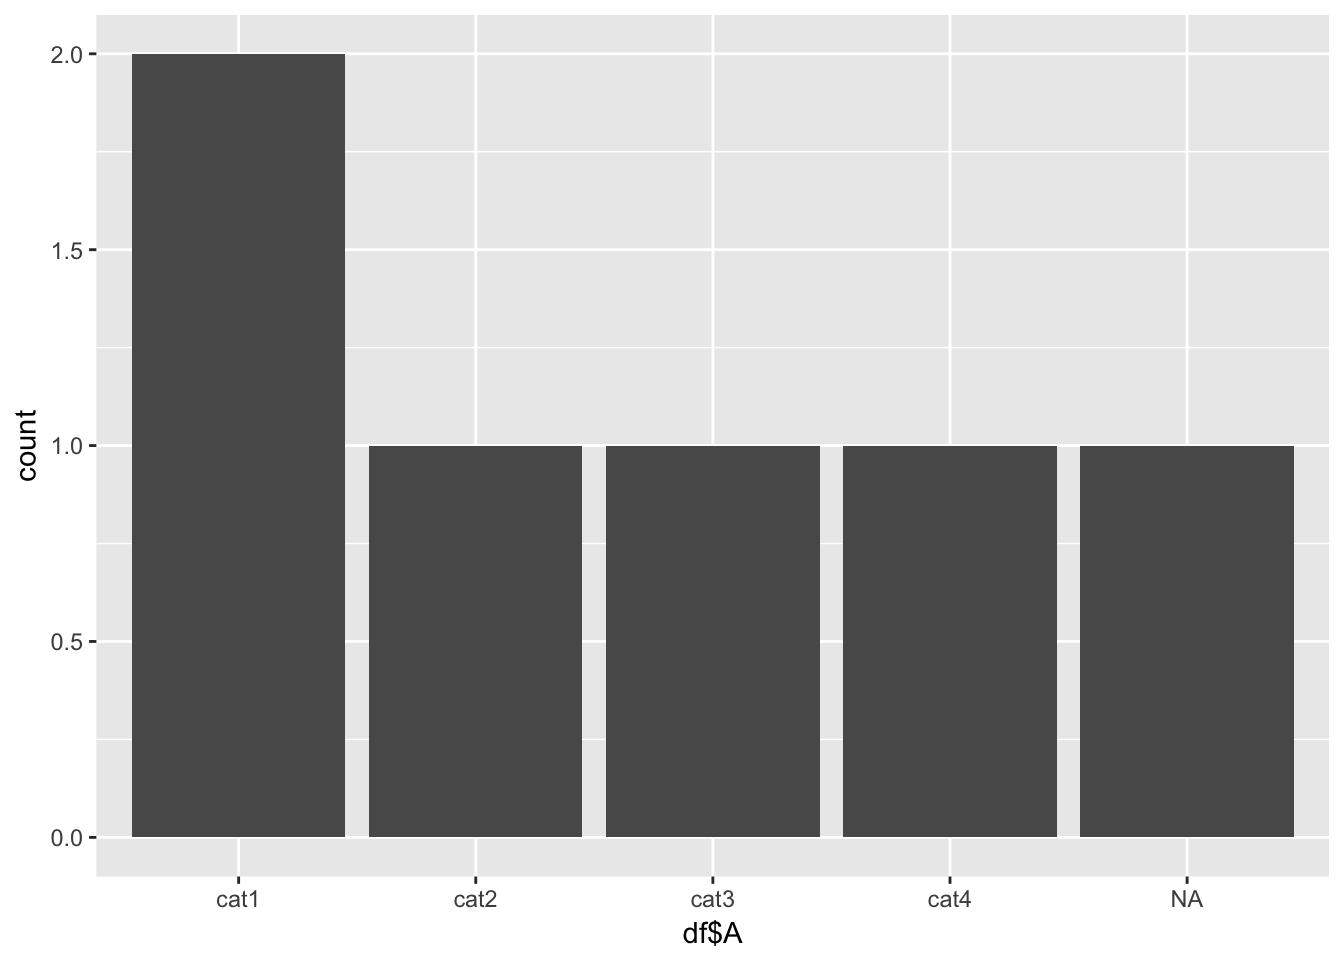
\includegraphics{_main_files/figure-latex/unnamed-chunk-57-1}

\begin{Shaded}
\begin{Highlighting}[]
\KeywordTok{qplot}\NormalTok{(df}\OperatorTok{$}\NormalTok{D, df}\OperatorTok{$}\NormalTok{B)  ## Makes a scatterplot}
\end{Highlighting}
\end{Shaded}

\begin{verbatim}
## Warning: Removed 1 rows containing missing values
## (geom_point).
\end{verbatim}

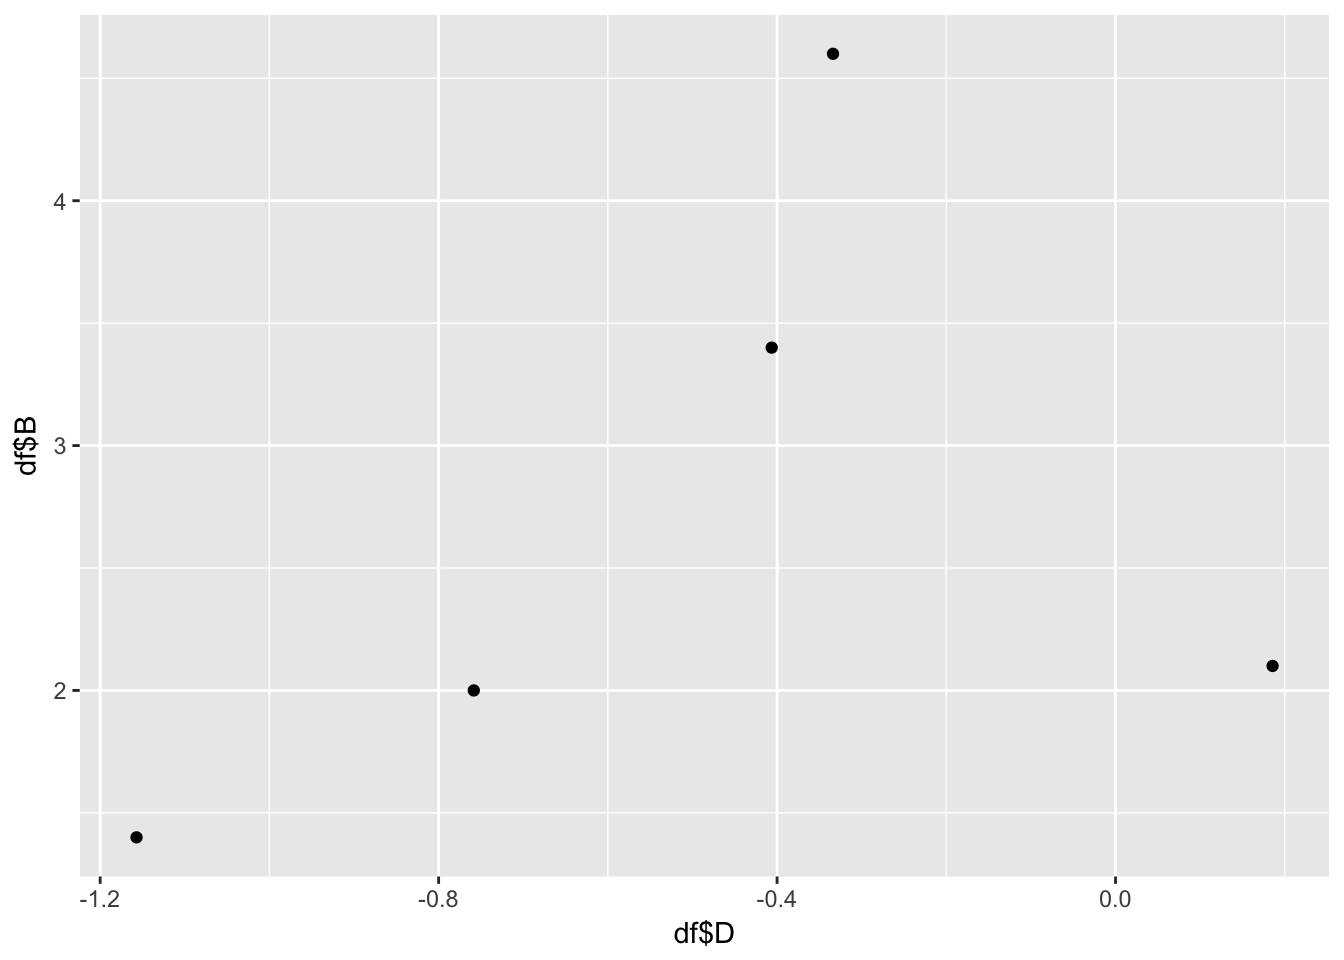
\includegraphics{_main_files/figure-latex/unnamed-chunk-57-2}

For a bit more control over the plot, you can use the \texttt{ggplot}
function. The first piece is the \texttt{ggplot} piece. From there, we
add layers. These layers generally start with \texttt{geom\_} then have
the type of plot.

Below, we start with telling \texttt{ggplot} the basics of the plot and
then build a boxplot. The x-axis is the variable ``C'' and the y-axis is
the variable ``D'' and then we color it by variable ``C'' as well.

\begin{Shaded}
\begin{Highlighting}[]
\KeywordTok{ggplot}\NormalTok{(df, }\KeywordTok{aes}\NormalTok{(}\DataTypeTok{x =}\NormalTok{ C, }\DataTypeTok{y =}\NormalTok{ D)) }\OperatorTok{+}\StringTok{ }\KeywordTok{geom_boxplot}\NormalTok{(}\KeywordTok{aes}\NormalTok{(}\DataTypeTok{color =}\NormalTok{ C))}
\end{Highlighting}
\end{Shaded}

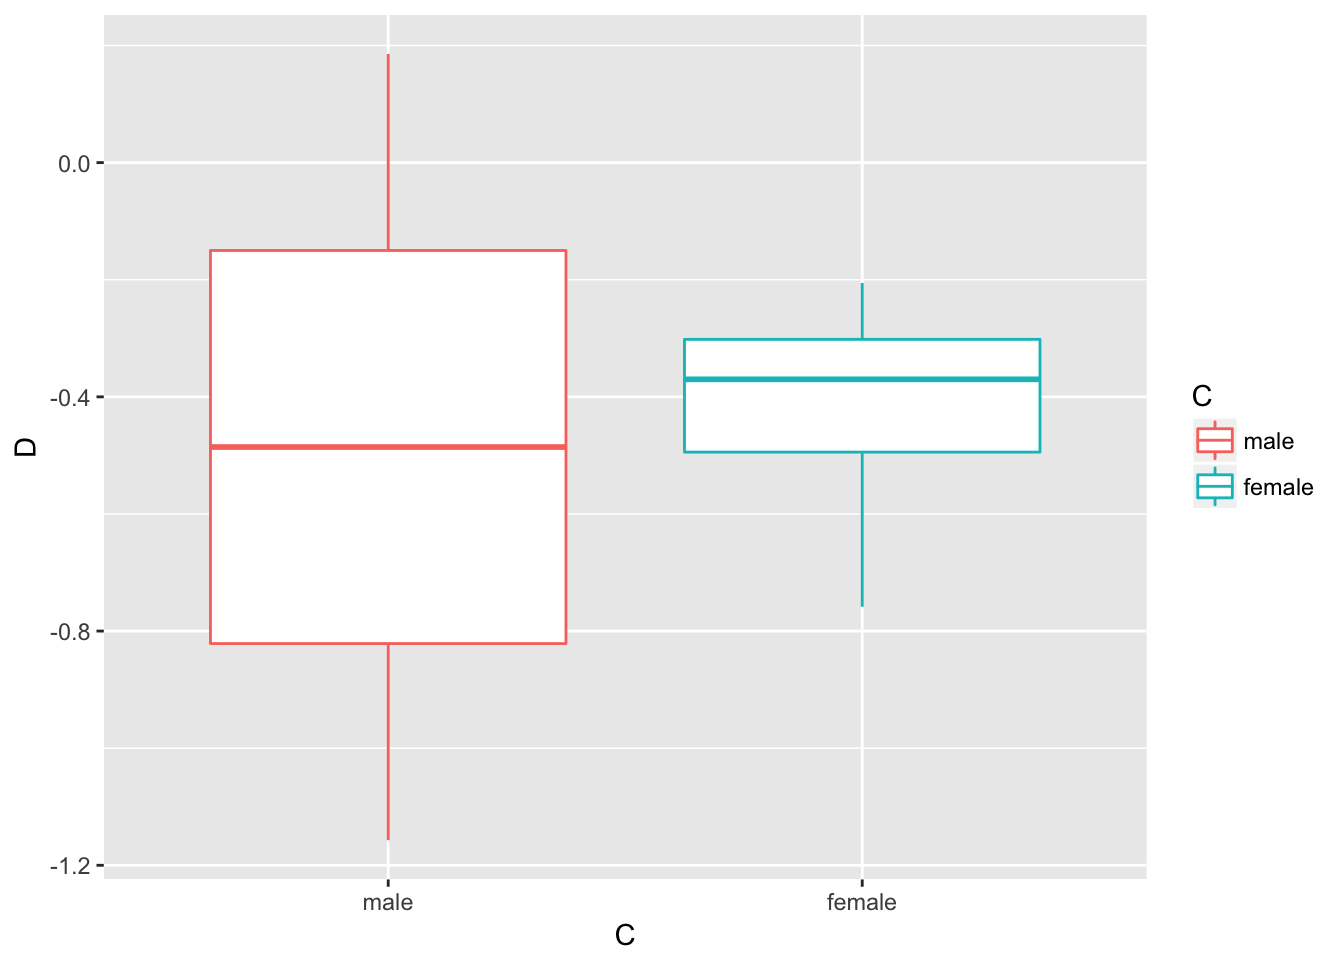
\includegraphics{_main_files/figure-latex/unnamed-chunk-58-1}

Here's a few more examples:

\begin{Shaded}
\begin{Highlighting}[]
\KeywordTok{ggplot}\NormalTok{(df, }\KeywordTok{aes}\NormalTok{(}\DataTypeTok{x =}\NormalTok{ C)) }\OperatorTok{+}\StringTok{ }\KeywordTok{geom_bar}\NormalTok{(}\DataTypeTok{stat =} \StringTok{"count"}\NormalTok{, }
    \KeywordTok{aes}\NormalTok{(}\DataTypeTok{fill =}\NormalTok{ C))}
\end{Highlighting}
\end{Shaded}

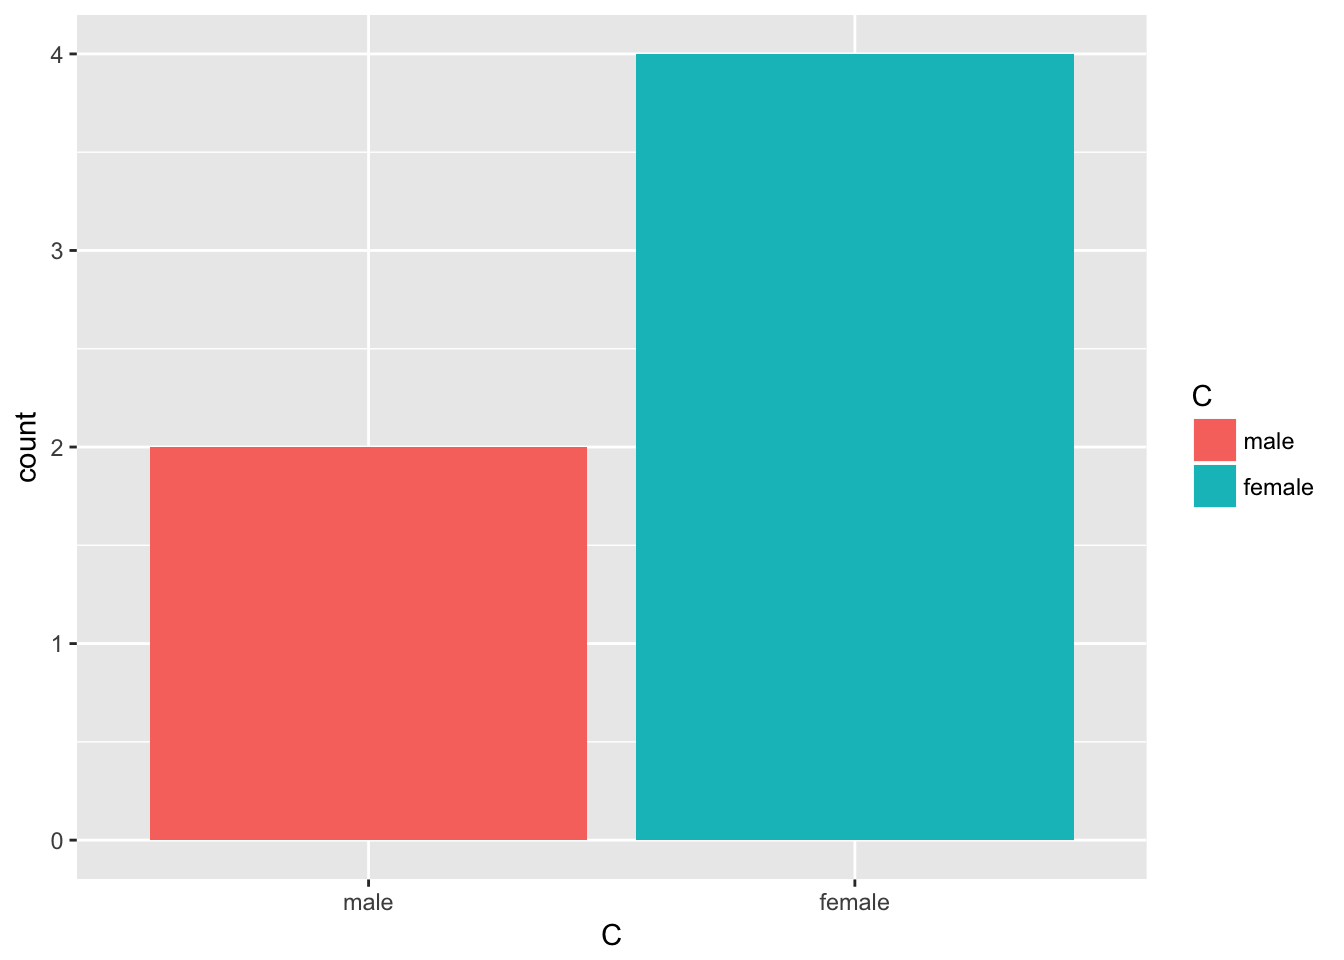
\includegraphics{_main_files/figure-latex/unnamed-chunk-59-1}

\begin{Shaded}
\begin{Highlighting}[]
\KeywordTok{ggplot}\NormalTok{(df, }\KeywordTok{aes}\NormalTok{(}\DataTypeTok{x =}\NormalTok{ B, }\DataTypeTok{y =}\NormalTok{ D)) }\OperatorTok{+}\StringTok{ }\KeywordTok{geom_point}\NormalTok{(}\KeywordTok{aes}\NormalTok{(}\DataTypeTok{color =}\NormalTok{ C))}
\end{Highlighting}
\end{Shaded}

\begin{verbatim}
## Warning: Removed 1 rows containing missing values
## (geom_point).
\end{verbatim}

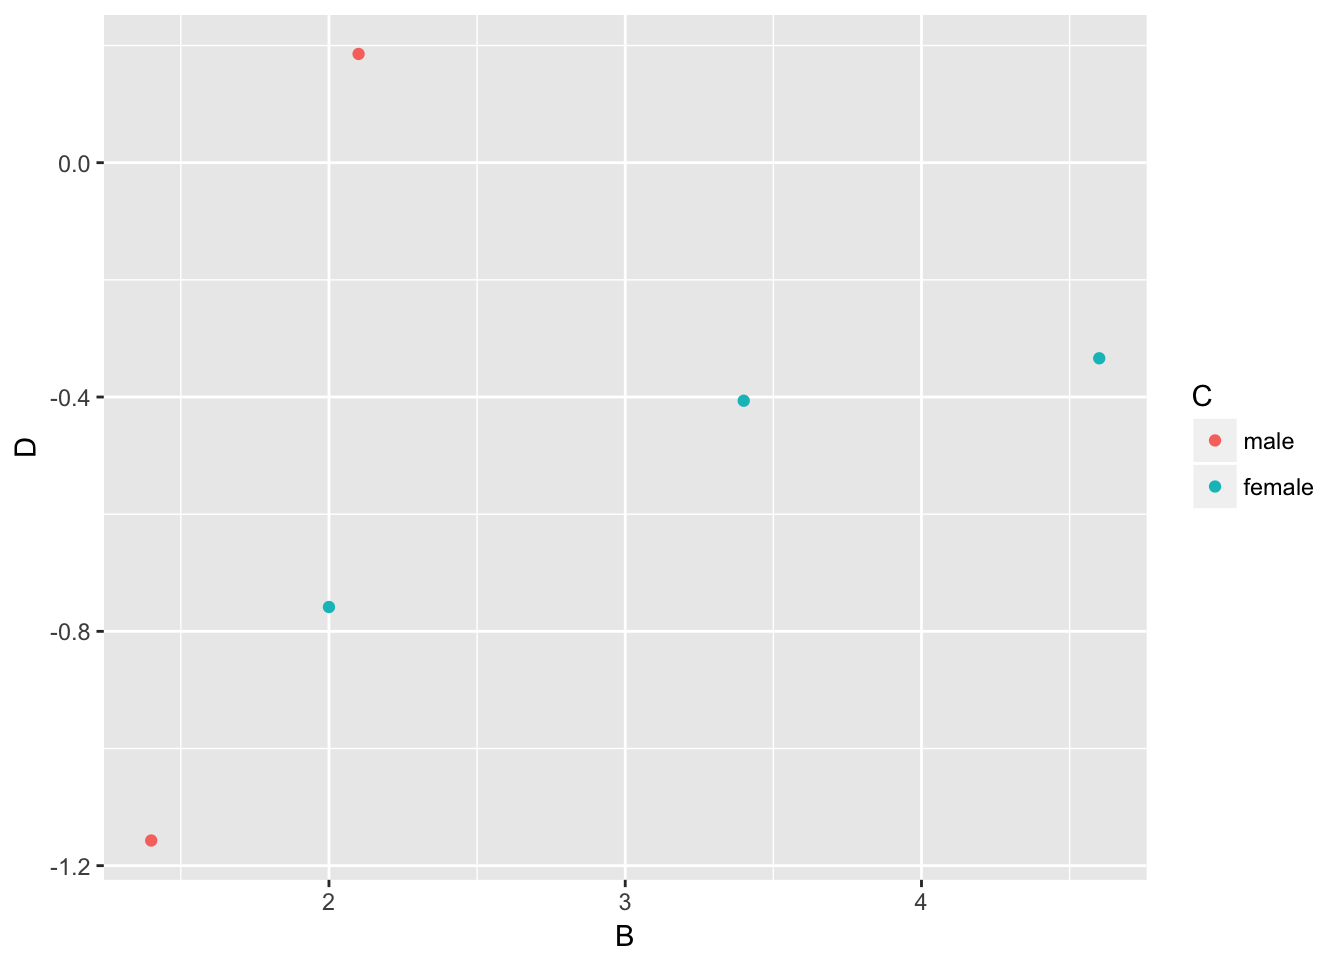
\includegraphics{_main_files/figure-latex/unnamed-chunk-60-1}

\emph{Note that the warning that says it removed a row is because we had
a missing value in ``C''.}

We are going to make the first one again but with some aesthetic
adjustments. Notice that we just added two extra lines telling
\texttt{ggplot2} how we want some things to look.\footnote{This is just
  scratching the surface of what we can change in the plots.}

\begin{Shaded}
\begin{Highlighting}[]
\KeywordTok{ggplot}\NormalTok{(df, }\KeywordTok{aes}\NormalTok{(}\DataTypeTok{x =}\NormalTok{ C, }\DataTypeTok{y =}\NormalTok{ D)) }\OperatorTok{+}\StringTok{ }\KeywordTok{geom_boxplot}\NormalTok{(}\KeywordTok{aes}\NormalTok{(}\DataTypeTok{color =}\NormalTok{ C)) }\OperatorTok{+}\StringTok{ }
\StringTok{    }\KeywordTok{theme_bw}\NormalTok{() }\OperatorTok{+}\StringTok{ }\KeywordTok{scale_color_manual}\NormalTok{(}\DataTypeTok{values =} \KeywordTok{c}\NormalTok{(}\StringTok{"dodgerblue4"}\NormalTok{, }
    \StringTok{"coral2"}\NormalTok{))}
\end{Highlighting}
\end{Shaded}

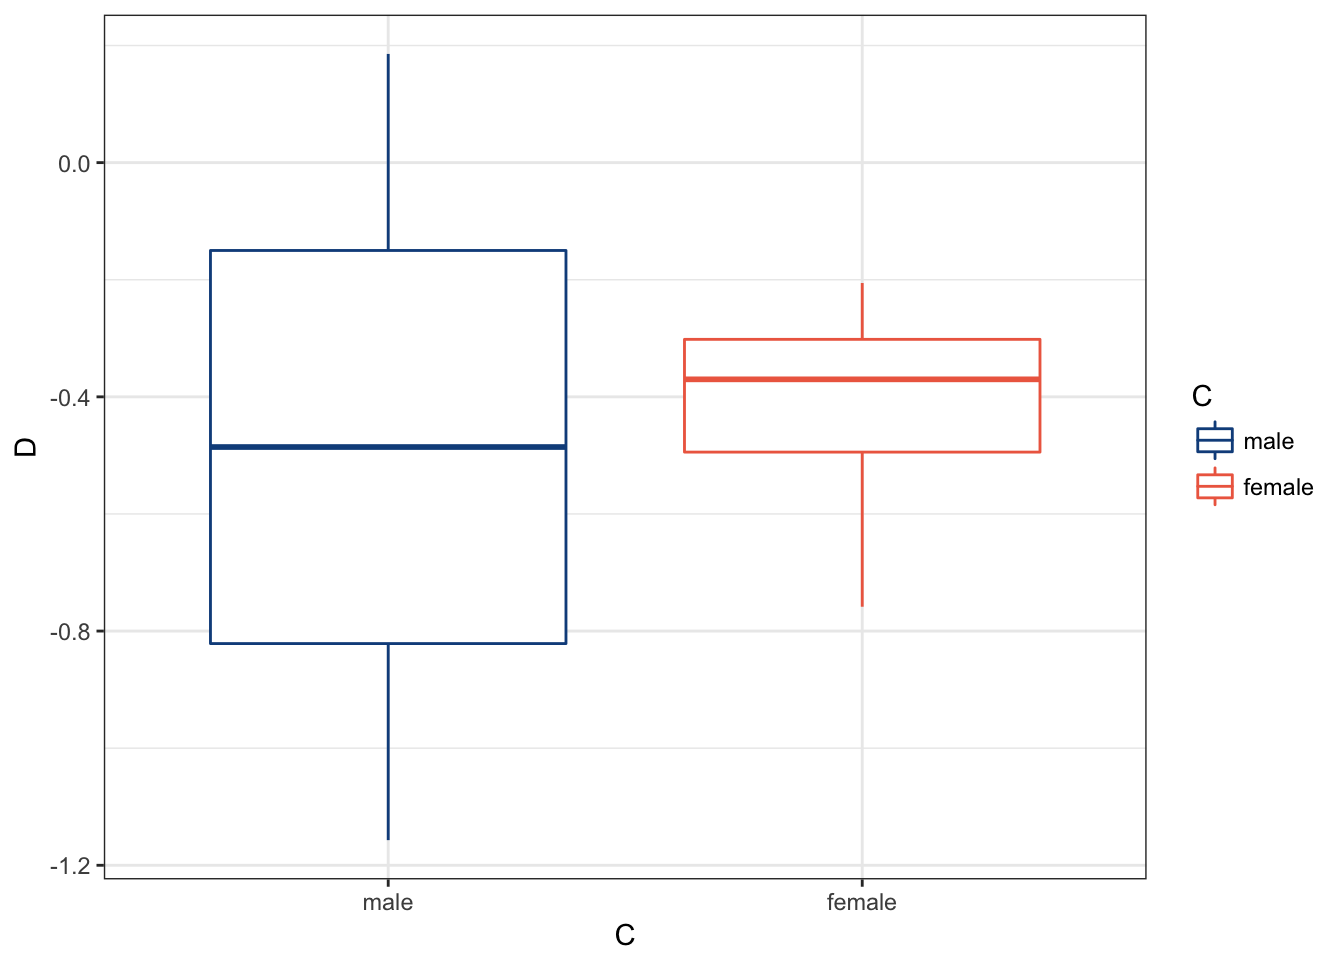
\includegraphics{_main_files/figure-latex/unnamed-chunk-61-1}

The \texttt{theme\_bw()} makes the background white, the
\texttt{scale\_color\_manual()} allows us to change the colors in the
plot. You can get a good idea of how many types of plots you can do by
going to
\href{http://docs.ggplot2.org/current/}{http://docs.ggplot2.org/current}.
Almost any informative plot that you need to do as a researcher is
possible with \texttt{ggplot2}.

We will be using \texttt{ggplot2} extensively in the book to help
understand our data and our models as well as communicate our results.

\chapter*{Chapter 4: Basic Analyses}\label{chapter-4-basic-analyses}
\addcontentsline{toc}{chapter}{Chapter 4: Basic Analyses}

\begin{quote}
``The goal is to turn data into information, and information into
insight.''

--- Carly Fiorina
\end{quote}

In this chapter we are going to demonstrate basic modeling in
\texttt{R}. Lucky for us, \texttt{R} is built for these analyses. It is
actually quite straight-forward to run these types of models and analyze
the output. Not only that, but there are simple ways to compare models.

We will go through the \textbf{ANOVA} family of analyses, the
\textbf{linear regression} models, and look at \textbf{diagnostics} of
each.

\section*{ANOVA}\label{anova}
\addcontentsline{toc}{section}{ANOVA}

ANOVA stands for \textbf{an}alysis \textbf{o}f \textbf{va}riance. It is
a family of methods (e.g.~ANCOVA, MANOVA) that all share the fact that
they compare a continuous dependent variable by a grouping factor
variable (and may have multiple outcomes or other covariates).

\[
Y_i = \alpha_0 + \alpha_1 \text{Group}_i + e_i
\] Since the groups are compared using ``effect coding,'' the
\(\alpha_0\) is the grand mean and each of the group level means are
compared to it.

To run an ANOVA model, you can simply use the \texttt{aov} function. In
the example below, we are analyzing whether family size (although not
fully continuous it is still useful for the example) differs by race.

\begin{Shaded}
\begin{Highlighting}[]
\NormalTok{df}\OperatorTok{$}\NormalTok{race <-}\StringTok{ }\KeywordTok{factor}\NormalTok{(df}\OperatorTok{$}\NormalTok{ridreth1, }\DataTypeTok{labels =} \KeywordTok{c}\NormalTok{(}\StringTok{"MexicanAmerican"}\NormalTok{, }
    \StringTok{"OtherHispanic"}\NormalTok{, }\StringTok{"White"}\NormalTok{, }\StringTok{"Black"}\NormalTok{, }\StringTok{"Other"}\NormalTok{))}
\NormalTok{df}\OperatorTok{$}\NormalTok{famsize <-}\StringTok{ }\KeywordTok{as.numeric}\NormalTok{(df}\OperatorTok{$}\NormalTok{dmdfmsiz)}

\NormalTok{fit <-}\StringTok{ }\KeywordTok{aov}\NormalTok{(famsize }\OperatorTok{~}\StringTok{ }\NormalTok{race, df)}
\KeywordTok{anova}\NormalTok{(fit)}
\end{Highlighting}
\end{Shaded}

\begin{verbatim}
## Analysis of Variance Table
## 
## Response: famsize
##             Df Sum Sq Mean Sq F value Pr(>F)
## race         4    541   135.3    51.4 <2e-16
## Residuals 4627  12187     2.6               
##              
## race      ***
## Residuals    
## ---
## Signif. codes:  
##   0 '***' 0.001 '**' 0.01 '*' 0.05 '.' 0.1  ' ' 1
\end{verbatim}

We make sure the variables are the right type, then we use the
\texttt{aov} function. Inside of the function we have what is called a
formula. It has the general structure:
\texttt{leftside\ \textasciitilde{}\ rightside}. Generally, the left
side is an outcome variable and the right side is the predictor
(i.e.~independent) variable. Here, we have \texttt{race} predicting
\texttt{famsize}. We assign the model to the name \texttt{fit} which is
a common way of denoting it is a model. Finally, we use the
\texttt{anova} function to output a nice ANOVA table.

In the output we see the normal ANOVA table and we can see the p-value
(\texttt{Pr(\textgreater{}F)}) is very, very small and thus is quite
significant. We can look at how the groups relate using a box plot. We
will be using some of the practice you got in Chapter 3 using
\texttt{ggplot2} for this.

\begin{Shaded}
\begin{Highlighting}[]
\KeywordTok{library}\NormalTok{(ggplot2)}

\KeywordTok{ggplot}\NormalTok{(df, }\KeywordTok{aes}\NormalTok{(}\DataTypeTok{x =}\NormalTok{ race, }\DataTypeTok{y =}\NormalTok{ famsize)) }\OperatorTok{+}\StringTok{ }\KeywordTok{geom_boxplot}\NormalTok{(}\KeywordTok{aes}\NormalTok{(}\DataTypeTok{color =}\NormalTok{ race)) }\OperatorTok{+}\StringTok{ }
\StringTok{    }\KeywordTok{scale_color_manual}\NormalTok{(}\DataTypeTok{guide =} \OtherTok{FALSE}\NormalTok{, }\DataTypeTok{values =} \KeywordTok{c}\NormalTok{(}\StringTok{"dodgerblue3"}\NormalTok{, }
        \StringTok{"coral2"}\NormalTok{, }\StringTok{"chartreuse4"}\NormalTok{, }\StringTok{"darkorchid"}\NormalTok{, }
        \StringTok{"firebrick2"}\NormalTok{)) }\OperatorTok{+}\StringTok{ }\KeywordTok{theme_bw}\NormalTok{()}
\end{Highlighting}
\end{Shaded}

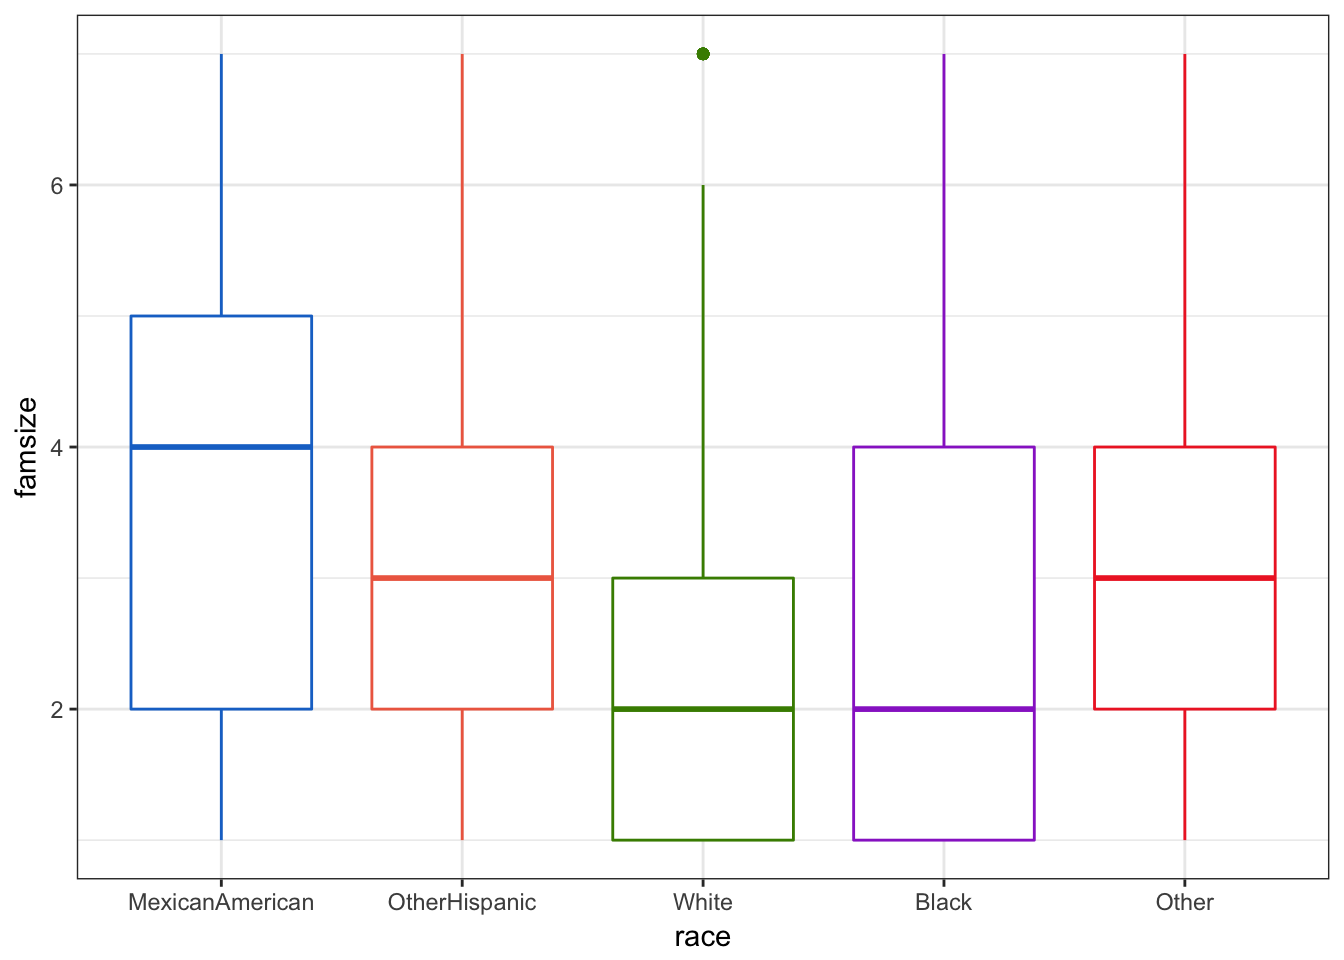
\includegraphics{_main_files/figure-latex/unnamed-chunk-64-1}

This immediately gives us an idea of where some differences may be
occuring. It would appear that ``White'' and ``MexicanAmerican'' groups
are different in family size.

\section*{Assumptions}\label{assumptions}
\addcontentsline{toc}{section}{Assumptions}

We also would like to make sure the assumptions look like they are being
met. In ANOVA, we want the residuals to be distributed normally, the
variance of each group should be approximately the same, the groups are
assumed to be randomly assigned, and the sample should be randomly
selected as well.

In \texttt{R} we can get some simple graphical checks using
\texttt{plot}. All we provide is our ANOVA object (here it is
\texttt{fit}). The line before it \texttt{par(mfrow=c(1,2))} tells
\texttt{R} to have two plots per row (the 1 means one row, 2 means two
columns).

\begin{Shaded}
\begin{Highlighting}[]
\KeywordTok{par}\NormalTok{(}\DataTypeTok{mfrow =} \KeywordTok{c}\NormalTok{(}\DecValTok{1}\NormalTok{, }\DecValTok{2}\NormalTok{))}
\KeywordTok{plot}\NormalTok{(fit)}
\end{Highlighting}
\end{Shaded}

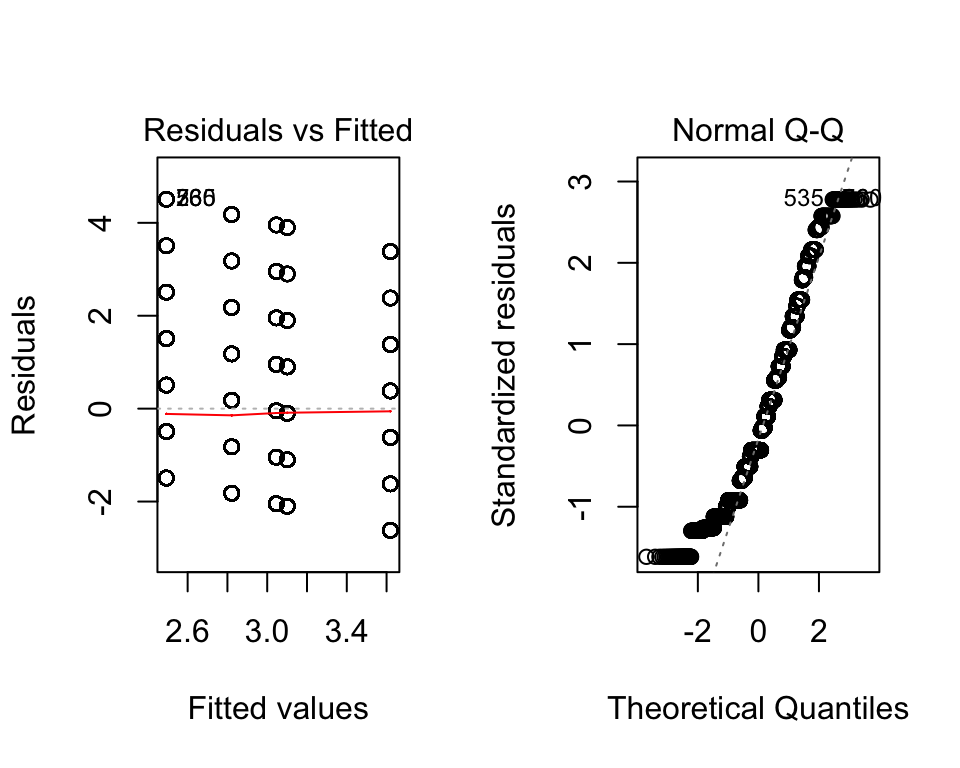
\includegraphics{_main_files/figure-latex/unnamed-chunk-65-1}
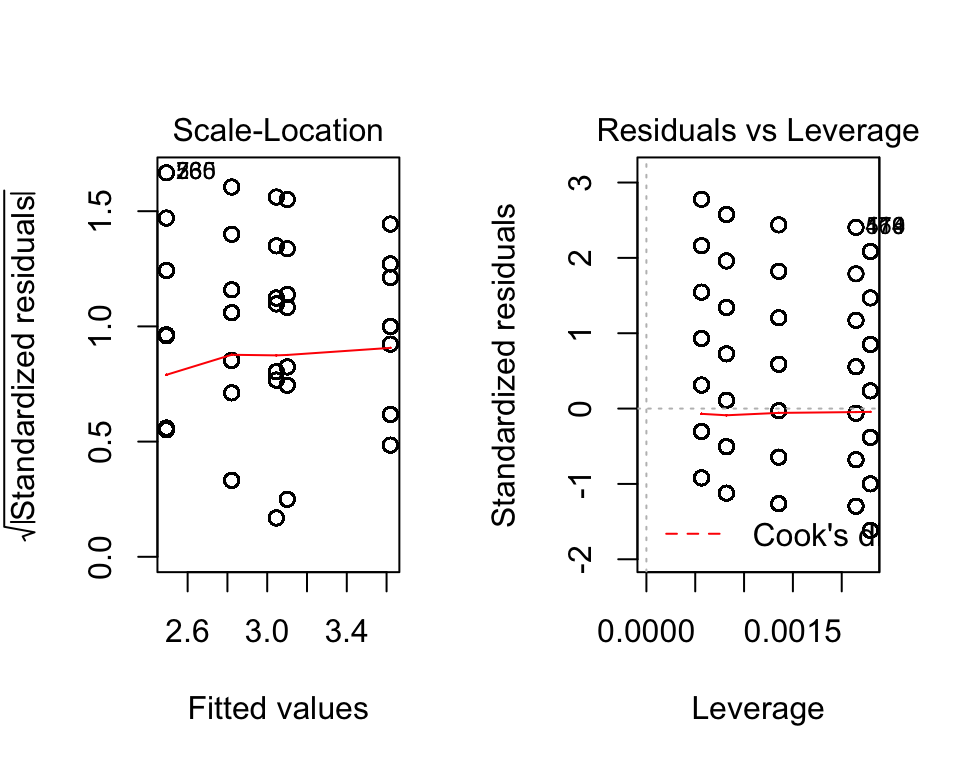
\includegraphics{_main_files/figure-latex/unnamed-chunk-65-2}

Here, it looks like we have a problem with normality (see the Normal Q-Q
plot). Those dots should approximately follow the dotted line, which is
not the case. In the first plot (Residuals vs.~Fitted) suggests we have
approximate homoskedasticity.

\section*{Linear Modeling}\label{linear-modeling}
\addcontentsline{toc}{section}{Linear Modeling}

Linear regression is nearly identical to ANOVA. In fact, a linear
regression with a continuous outcome and categorical predictor is
exactly the same (if we use effect coding). For example, if we run the
same model but with the linear regression function \texttt{lm} we get
the same ANOVA table.

\begin{Shaded}
\begin{Highlighting}[]
\NormalTok{fit2 <-}\StringTok{ }\KeywordTok{lm}\NormalTok{(famsize }\OperatorTok{~}\StringTok{ }\NormalTok{race, }\DataTypeTok{data =}\NormalTok{ df)}
\KeywordTok{anova}\NormalTok{(fit2)}
\end{Highlighting}
\end{Shaded}

\begin{verbatim}
## Analysis of Variance Table
## 
## Response: famsize
##             Df Sum Sq Mean Sq F value Pr(>F)
## race         4    541   135.3    51.4 <2e-16
## Residuals 4627  12187     2.6               
##              
## race      ***
## Residuals    
## ---
## Signif. codes:  
##   0 '***' 0.001 '**' 0.01 '*' 0.05 '.' 0.1  ' ' 1
\end{verbatim}

Surprise! It is the same as before. Here we can also use the
\texttt{summary} function and we get the coefficients in the model as
well (using dummy coding). The first level of the categorical variable
is the reference group (the group that the others are compared to). We
also get the intercept (in this case, the average value of the reference
group).

\begin{Shaded}
\begin{Highlighting}[]
\KeywordTok{summary}\NormalTok{(fit2)}
\end{Highlighting}
\end{Shaded}

\begin{verbatim}
## 
## Call:
## lm(formula = famsize ~ race, data = df)
## 
## Residuals:
##    Min     1Q Median     3Q    Max 
## -2.619 -1.493 -0.493  0.954  4.507 
## 
## Coefficients:
##                   Estimate Std. Error
## (Intercept)         3.6193     0.0777
## raceOtherHispanic  -0.5184     0.1081
## raceWhite          -1.1260     0.0868
## raceBlack          -0.7980     0.0906
## raceOther          -0.5732     0.0980
##                   t value Pr(>|t|)    
## (Intercept)         46.56  < 2e-16 ***
## raceOtherHispanic   -4.79  1.7e-06 ***
## raceWhite          -12.98  < 2e-16 ***
## raceBlack           -8.81  < 2e-16 ***
## raceOther           -5.85  5.3e-09 ***
## ---
## Signif. codes:  
##   0 '***' 0.001 '**' 0.01 '*' 0.05 '.' 0.1  ' ' 1
## 
## Residual standard error: 1.62 on 4627 degrees of freedom
## Multiple R-squared:  0.0425, Adjusted R-squared:  0.0417 
## F-statistic: 51.4 on 4 and 4627 DF,  p-value: <2e-16
\end{verbatim}

\section*{Assumptions}\label{assumptions-1}
\addcontentsline{toc}{section}{Assumptions}

Linear regression has a few important assumptions, often called
``Gauss-Markov Assumptions''. These include:

\begin{enumerate}
\def\labelenumi{\arabic{enumi}.}
\tightlist
\item
  The model is linear in parameters.
\item
  Homoskedasticity (i.e.~the variance of the residual is roughly uniform
  across the values of the independents).
\item
  Normality of residuals.
\end{enumerate}

Numbers 2 and 3 are fairly easy to assess using the \texttt{plot()}
function on the model object as we did with the ANOVA model. The linear
in parameters suggests that the relationship between the outcome and
independents is linear.

\begin{Shaded}
\begin{Highlighting}[]
\KeywordTok{par}\NormalTok{(}\DataTypeTok{mfrow =} \KeywordTok{c}\NormalTok{(}\DecValTok{1}\NormalTok{, }\DecValTok{2}\NormalTok{))}
\KeywordTok{plot}\NormalTok{(fit2)}
\end{Highlighting}
\end{Shaded}

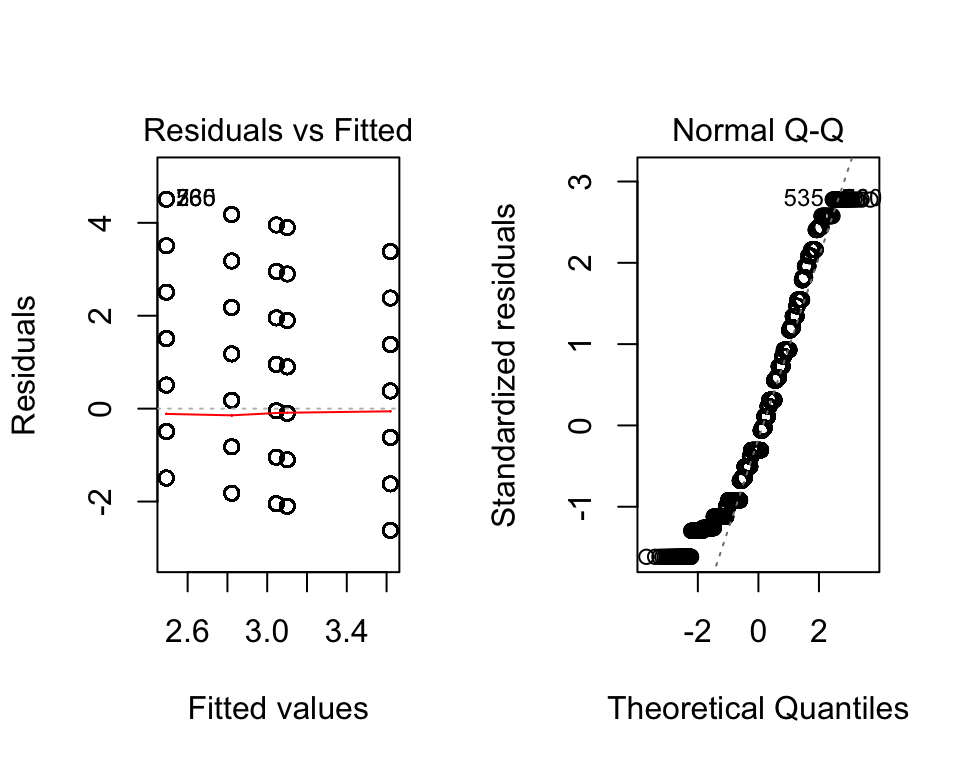
\includegraphics{_main_files/figure-latex/unnamed-chunk-68-1}
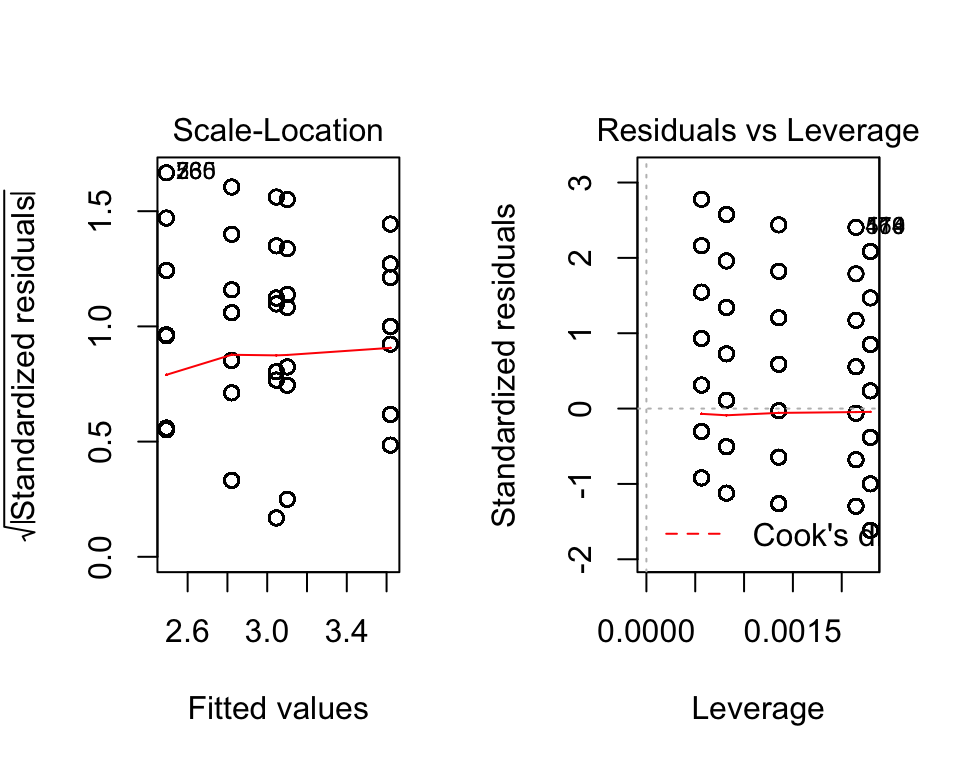
\includegraphics{_main_files/figure-latex/unnamed-chunk-68-2}

\section*{Comparing Models}\label{comparing-models}
\addcontentsline{toc}{section}{Comparing Models}

Often when running linear regression, we want to compare models and see
if one fits significantly better than another. We also often want to
present all the models in a table to let our readers compare the models.
We will demonstrate both.

\subsection*{Compare Statistically}\label{compare-statistically}
\addcontentsline{toc}{subsection}{Compare Statistically}

Using the \texttt{anova()} function, we can compare models
statistically.

\begin{Shaded}
\begin{Highlighting}[]
\KeywordTok{anova}\NormalTok{(fit, fit2)}
\end{Highlighting}
\end{Shaded}

\begin{verbatim}
## Analysis of Variance Table
## 
## Model 1: famsize ~ race
## Model 2: famsize ~ race
##   Res.Df   RSS Df Sum of Sq F Pr(>F)
## 1   4627 12187                      
## 2   4627 12187  0         0
\end{verbatim}

The \texttt{anova()} function works with all sorts of modeling schemes
and can help in model selection. Not surprisingly, when we compared the
ANOVA and the simple linear model, they are \emph{exactly} the same in
overall model terms (the only difference is in how the cateogrical
variable is coded---either effect coding in ANOVA or dummy coding in
regression). For a more interesting comparison, lets run a new model
with an additional variable and then make a comparison.

\begin{Shaded}
\begin{Highlighting}[]
\NormalTok{fit3 =}\StringTok{ }\KeywordTok{lm}\NormalTok{(famsize }\OperatorTok{~}\StringTok{ }\NormalTok{race }\OperatorTok{+}\StringTok{ }\NormalTok{marriage, }\DataTypeTok{data =}\NormalTok{ df)}
\KeywordTok{summary}\NormalTok{(fit3)}
\end{Highlighting}
\end{Shaded}

\begin{verbatim}
## 
## Call:
## lm(formula = famsize ~ race + marriage, data = df)
## 
## Residuals:
##    Min     1Q Median     3Q    Max 
##  -2.97  -1.18  -0.41   1.03   5.29 
## 
## Coefficients:
##                   Estimate Std. Error
## (Intercept)         3.9689     0.0779
## raceOtherHispanic  -0.4118     0.1037
## raceWhite          -1.0268     0.0836
## raceBlack          -0.5588     0.0879
## raceOther          -0.5624     0.0946
## marriage2          -1.2291     0.0867
## marriage3          -1.2025     0.0778
## marriage4          -0.4775     0.1253
## marriage5          -0.8093     0.0597
## marriage6          -0.4921     0.0887
##                   t value Pr(>|t|)    
## (Intercept)         50.95  < 2e-16 ***
## raceOtherHispanic   -3.97  7.2e-05 ***
## raceWhite          -12.28  < 2e-16 ***
## raceBlack           -6.36  2.3e-10 ***
## raceOther           -5.94  3.0e-09 ***
## marriage2          -14.18  < 2e-16 ***
## marriage3          -15.45  < 2e-16 ***
## marriage4           -3.81  0.00014 ***
## marriage5          -13.56  < 2e-16 ***
## marriage6           -5.55  3.0e-08 ***
## ---
## Signif. codes:  
##   0 '***' 0.001 '**' 0.01 '*' 0.05 '.' 0.1  ' ' 1
## 
## Residual standard error: 1.55 on 4622 degrees of freedom
## Multiple R-squared:  0.126,  Adjusted R-squared:  0.124 
## F-statistic: 73.7 on 9 and 4622 DF,  p-value: <2e-16
\end{verbatim}

Notice that the variable is associated with the outcome according to the
t-test seen in the summary. So we would expect that \texttt{fit3} is
better than \texttt{fit2} at explaining the outcome, which we see in the
output below.

\begin{Shaded}
\begin{Highlighting}[]
\KeywordTok{anova}\NormalTok{(fit2, fit3)}
\end{Highlighting}
\end{Shaded}

\begin{verbatim}
## Analysis of Variance Table
## 
## Model 1: famsize ~ race
## Model 2: famsize ~ race + marriage
##   Res.Df   RSS Df Sum of Sq    F Pr(>F)    
## 1   4627 12187                             
## 2   4622 11131  5      1057 87.8 <2e-16 ***
## ---
## Signif. codes:  
##   0 '***' 0.001 '**' 0.01 '*' 0.05 '.' 0.1  ' ' 1
\end{verbatim}

\subsection*{Compare in a Table}\label{compare-in-a-table}
\addcontentsline{toc}{subsection}{Compare in a Table}

We can also compare the models in a well-formatted table that makes many
aspects easy to compare. Two main packages allow us to compare models:

\begin{enumerate}
\def\labelenumi{\arabic{enumi}.}
\tightlist
\item
  \texttt{stargazer}
\item
  \texttt{texreg}
\end{enumerate}

Both provide simple functions to compare multiple models. For example,
\texttt{stargazer} provides:

\begin{Shaded}
\begin{Highlighting}[]
\KeywordTok{library}\NormalTok{(stargazer)}
\KeywordTok{stargazer}\NormalTok{(fit2, fit3, }\DataTypeTok{type =} \StringTok{"text"}\NormalTok{)}
\end{Highlighting}
\end{Shaded}

\begin{verbatim}
## 
## =====================================================================
##                                    Dependent variable:               
##                     -------------------------------------------------
##                                          famsize                     
##                               (1)                      (2)           
## ---------------------------------------------------------------------
## raceOtherHispanic          -0.518***                -0.412***        
##                             (0.108)                  (0.104)         
##                                                                      
## raceWhite                  -1.130***                -1.030***        
##                             (0.087)                  (0.084)         
##                                                                      
## raceBlack                  -0.798***                -0.559***        
##                             (0.091)                  (0.088)         
##                                                                      
## raceOther                  -0.573***                -0.562***        
##                             (0.098)                  (0.095)         
##                                                                      
## marriage2                                           -1.230***        
##                                                      (0.087)         
##                                                                      
## marriage3                                           -1.200***        
##                                                      (0.078)         
##                                                                      
## marriage4                                           -0.477***        
##                                                      (0.125)         
##                                                                      
## marriage5                                           -0.809***        
##                                                      (0.060)         
##                                                                      
## marriage6                                           -0.492***        
##                                                      (0.089)         
##                                                                      
## Constant                    3.620***                 3.970***        
##                             (0.078)                  (0.078)         
##                                                                      
## ---------------------------------------------------------------------
## Observations                 4,632                    4,632          
## R2                           0.043                    0.126          
## Adjusted R2                  0.042                    0.124          
## Residual Std. Error    1.620 (df = 4627)        1.550 (df = 4622)    
## F Statistic         51.400*** (df = 4; 4627) 73.700*** (df = 9; 4622)
## =====================================================================
## Note:                                     *p<0.1; **p<0.05; ***p<0.01
\end{verbatim}

\section*{When Assumptions Fail}\label{when-assumptions-fail}
\addcontentsline{toc}{section}{When Assumptions Fail}

There are many things we can try when our assumptions fail. In my
opinion, the best and most interpretable way is to use a Generalized
Linear Model (GLM) which is discussed in the next chapter. There are a
few other things you can try which I'll show here. But, keep in mind
that these things can cause other problems. For example, to fix
normality we may accidentally cause heteroskedasticity. With that in
mind, here are some common methods to help a model fit better.

\subsection*{Log-Linear, Log-Log, Linear-Log,
Other}\label{log-linear-log-log-linear-log-other}
\addcontentsline{toc}{subsection}{Log-Linear, Log-Log, Linear-Log,
Other}

Sounds like a great tongue-twister? Well, it is but it's also three ways
of specifying (i.e.~deciding what is in) your model better.

\textbf{Log-Linear} is where we adjust the outcome variable by a natural
log transformation. This is done easily in \texttt{R}:

\begin{Shaded}
\begin{Highlighting}[]
\NormalTok{df}\OperatorTok{$}\NormalTok{log_outcome <-}\StringTok{ }\KeywordTok{log}\NormalTok{(df}\OperatorTok{$}\NormalTok{outcome)}

\KeywordTok{lm}\NormalTok{(log_outcome }\OperatorTok{~}\StringTok{ }\NormalTok{var1, }\DataTypeTok{data =}\NormalTok{ df)}
\end{Highlighting}
\end{Shaded}

\textbf{Log-Log} is where we adjust both the outcome and the predictor
variable with a log transformation. This is also easily done:

\begin{Shaded}
\begin{Highlighting}[]
\NormalTok{df}\OperatorTok{$}\NormalTok{log_outcome <-}\StringTok{ }\KeywordTok{log}\NormalTok{(df}\OperatorTok{$}\NormalTok{outcome)}
\NormalTok{df}\OperatorTok{$}\NormalTok{log_var1 <-}\StringTok{ }\KeywordTok{log}\NormalTok{(df}\OperatorTok{$}\NormalTok{var1)}

\KeywordTok{lm}\NormalTok{(log_outcome }\OperatorTok{~}\StringTok{ }\NormalTok{log_var1, }\DataTypeTok{data =}\NormalTok{ df)}
\end{Highlighting}
\end{Shaded}

\textbf{Linear-Log} is where we adjsut just the predictor variable with
a log transformation. And, you guessed it, this is easily done in
\texttt{R}:

\begin{Shaded}
\begin{Highlighting}[]
\NormalTok{df}\OperatorTok{$}\NormalTok{log_var1 <-}\StringTok{ }\KeywordTok{log}\NormalTok{(df}\OperatorTok{$}\NormalTok{var1)}

\KeywordTok{lm}\NormalTok{(outcome }\OperatorTok{~}\StringTok{ }\NormalTok{log_var1 }\OperatorTok{+}\StringTok{ }\NormalTok{var2, }\DataTypeTok{data =}\NormalTok{ df)}
\end{Highlighting}
\end{Shaded}

\textbf{Other} methods such as square rooting the outcome or using some
power function (e.g.~square, cube) are also quite common. There are
functions that look for the best transformation to use. However, I will
not cover it here since I think GLM's are better. So if you want to
learn about other ways to help your linear model go to the next chapter.

\section*{Interactions}\label{interactions}
\addcontentsline{toc}{section}{Interactions}

Many times hypotheses dealing with human beings include interactions
between effects. Interactions are when the effect of one variable
depends on another variable. For example, the effect of marital status
on family size may depend on whether the individual is a minority. In
fact, this is the hypothesis we'll test below.

Including interactions in ANOVA and regression type models are very
simple in \texttt{R}. Since interpretations of interaction effects are
often best through plots, we will also show simple methods to visualize
the interactions as well.

\subsection*{Interactions in ANOVA}\label{interactions-in-anova}
\addcontentsline{toc}{subsection}{Interactions in ANOVA}

In general, we refer to ANOVA's with interactions as ``2-way Factorial
ANOVA's''. We interact race and marriage status in this ANOVA. For
simplicity, we created a binary race variable called minority using the
\texttt{ifelse()} function. We explain this in more depth in Chapter 5.

\begin{Shaded}
\begin{Highlighting}[]
\NormalTok{df}\OperatorTok{$}\NormalTok{minority <-}\StringTok{ }\KeywordTok{factor}\NormalTok{(}\KeywordTok{ifelse}\NormalTok{(df}\OperatorTok{$}\NormalTok{race }\OperatorTok{==}\StringTok{ "White"}\NormalTok{, }
    \DecValTok{0}\NormalTok{, }\DecValTok{1}\NormalTok{), }\DataTypeTok{labels =} \KeywordTok{c}\NormalTok{(}\StringTok{"White"}\NormalTok{, }\StringTok{"Minority"}\NormalTok{))}
\NormalTok{fit_anova <-}\StringTok{ }\KeywordTok{aov}\NormalTok{(famsize }\OperatorTok{~}\StringTok{ }\NormalTok{minority }\OperatorTok{*}\StringTok{ }\NormalTok{marriage, }
\NormalTok{    df)}
\KeywordTok{anova}\NormalTok{(fit_anova)}
\end{Highlighting}
\end{Shaded}

\begin{verbatim}
## Analysis of Variance Table
## 
## Response: famsize
##                     Df Sum Sq Mean Sq
## minority             1    335     335
## marriage             5   1153     231
## minority:marriage    5     25       5
## Residuals         4620  11216       2
##                   F value Pr(>F)    
## minority           137.96 <2e-16 ***
## marriage            95.01 <2e-16 ***
## minority:marriage    2.05  0.068 .  
## Residuals                           
## ---
## Signif. codes:  
##   0 '***' 0.001 '**' 0.01 '*' 0.05 '.' 0.1  ' ' 1
\end{verbatim}

Notice two things: First, the interaction is significant (p = .003).
This is important since we are going to try to interpret this
interaction. Second, by including \texttt{minority*marriage} we get both
the main effects and the interaction. This is very important for
interpretation purposes so you can thank \texttt{R} for making it a bit
more easy on you.

We can check the assumptions the same way as before:

\begin{Shaded}
\begin{Highlighting}[]
\KeywordTok{par}\NormalTok{(}\DataTypeTok{mfrow =} \KeywordTok{c}\NormalTok{(}\DecValTok{1}\NormalTok{, }\DecValTok{2}\NormalTok{))}
\KeywordTok{plot}\NormalTok{(fit_anova)}
\end{Highlighting}
\end{Shaded}

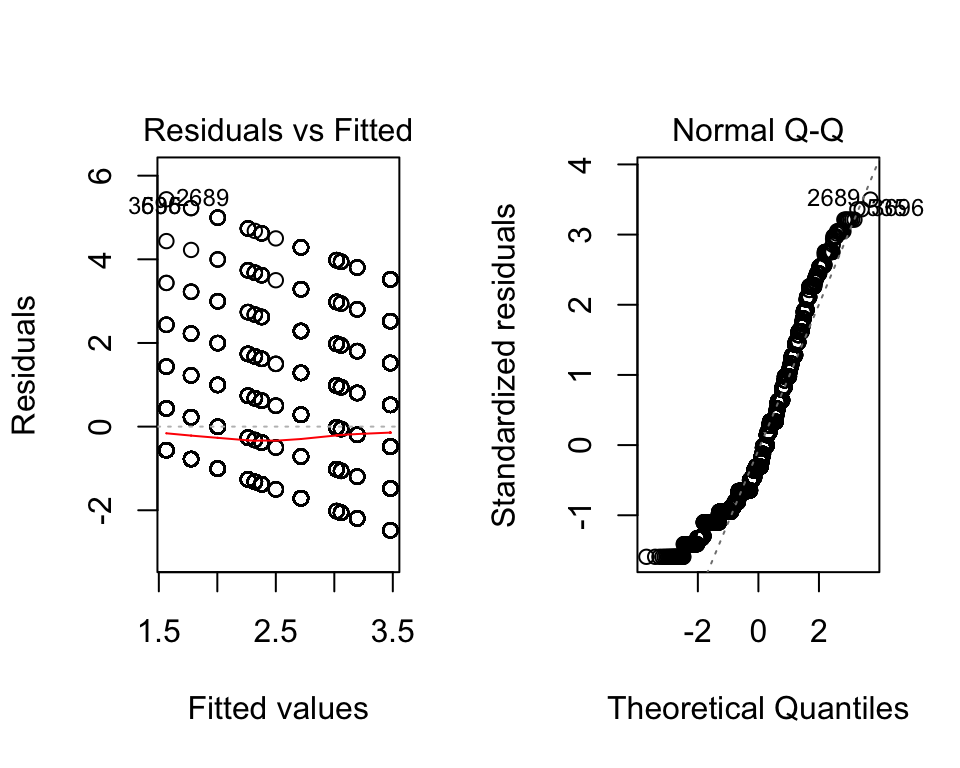
\includegraphics{_main_files/figure-latex/unnamed-chunk-77-1}
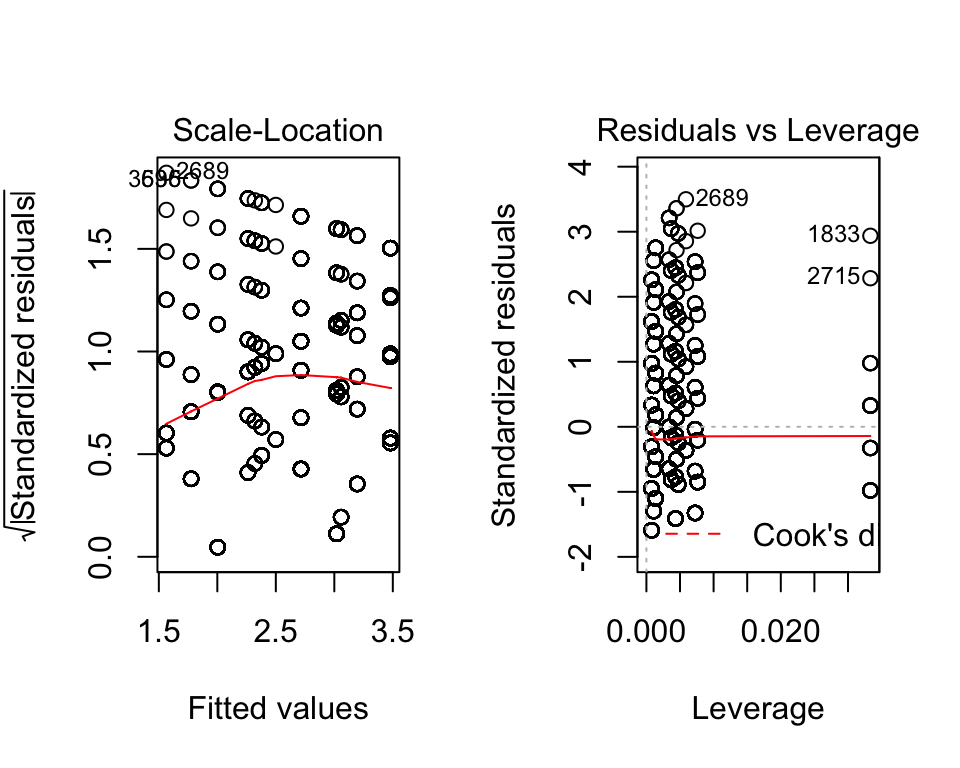
\includegraphics{_main_files/figure-latex/unnamed-chunk-77-2} Again, the
assumptions are not met for this model. But, if we ignore that for now,
we can quickly find a way to interpret the interaction.

We first create a new data set that is composed of every possible
combination of the variables in the model. This allows us to get
unbiased estimates for the plotting.

\begin{Shaded}
\begin{Highlighting}[]
\NormalTok{newdata <-}\StringTok{ }\KeywordTok{expand.grid}\NormalTok{(}\DataTypeTok{minority =} \KeywordTok{levels}\NormalTok{(df}\OperatorTok{$}\NormalTok{minority), }
    \DataTypeTok{marriage =} \KeywordTok{levels}\NormalTok{(df}\OperatorTok{$}\NormalTok{marriage))}
\NormalTok{newdata}\OperatorTok{$}\NormalTok{preds <-}\StringTok{ }\KeywordTok{predict}\NormalTok{(fit_anova, }\DataTypeTok{newdata =}\NormalTok{ newdata)}
\end{Highlighting}
\end{Shaded}

We now use \texttt{ggplot2} just as before.

\begin{Shaded}
\begin{Highlighting}[]
\KeywordTok{ggplot}\NormalTok{(newdata, }\KeywordTok{aes}\NormalTok{(}\DataTypeTok{x =}\NormalTok{ marriage, }\DataTypeTok{y =}\NormalTok{ preds, }\DataTypeTok{group =}\NormalTok{ minority)) }\OperatorTok{+}\StringTok{ }
\StringTok{    }\KeywordTok{geom_line}\NormalTok{(}\KeywordTok{aes}\NormalTok{(}\DataTypeTok{color =}\NormalTok{ minority)) }\OperatorTok{+}\StringTok{ }\KeywordTok{geom_point}\NormalTok{(}\KeywordTok{aes}\NormalTok{(}\DataTypeTok{color =}\NormalTok{ minority)) }\OperatorTok{+}\StringTok{ }
\StringTok{    }\KeywordTok{labs}\NormalTok{(}\DataTypeTok{y =} \StringTok{"Predicted Family Size"}\NormalTok{, }\DataTypeTok{x =} \StringTok{"Marital Status"}\NormalTok{) }\OperatorTok{+}\StringTok{ }
\StringTok{    }\KeywordTok{scale_color_manual}\NormalTok{(}\DataTypeTok{name =} \StringTok{""}\NormalTok{, }\DataTypeTok{values =} \KeywordTok{c}\NormalTok{(}\StringTok{"dodgerblue3"}\NormalTok{, }
        \StringTok{"chartreuse3"}\NormalTok{)) }\OperatorTok{+}\StringTok{ }\KeywordTok{theme_anteo_wh}\NormalTok{()  ## from anteo package}
\end{Highlighting}
\end{Shaded}

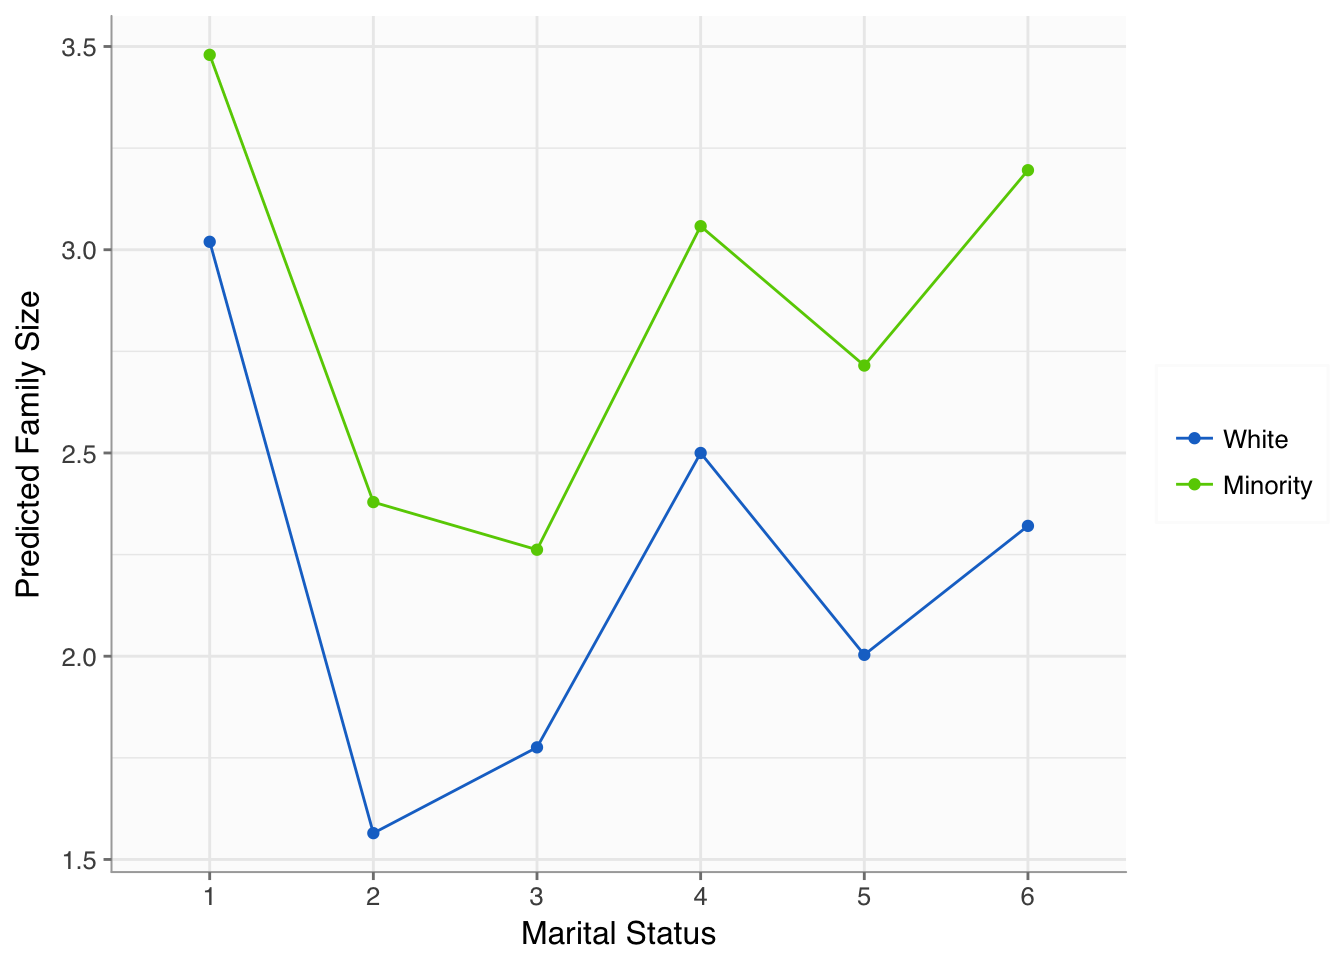
\includegraphics{_main_files/figure-latex/unnamed-chunk-79-1}

The plot tells use a handful of things. For example, we see minorities
generally have more children across marital statuses. However, the
difference is smaller for married and divorced individuals compared to
widowed, separated, never married, and living with a partner. There's
certainly more to gleen from the plot, but we won't waste your time.

\subsection*{Interactions in Linear
Regression}\label{interactions-in-linear-regression}
\addcontentsline{toc}{subsection}{Interactions in Linear Regression}

Interactions in linear regression is nearly identical as in ANOVA,
except we use dummy coding. It provides a bit more information. For
example, we get the coefficients from the linear regression whereas the
ANOVA does not provide this. We can run a regression model via:

\begin{Shaded}
\begin{Highlighting}[]
\NormalTok{fit_reg <-}\StringTok{ }\KeywordTok{lm}\NormalTok{(famsize }\OperatorTok{~}\StringTok{ }\NormalTok{minority }\OperatorTok{*}\StringTok{ }\NormalTok{marriage, df)}
\KeywordTok{summary}\NormalTok{(fit_reg)}
\end{Highlighting}
\end{Shaded}

\begin{verbatim}
## 
## Call:
## lm(formula = famsize ~ minority * marriage, data = df)
## 
## Residuals:
##    Min     1Q Median     3Q    Max 
## -2.479 -1.196 -0.479  0.980  5.435 
## 
## Coefficients:
##                            Estimate
## (Intercept)                  3.0195
## minorityMinority             0.4599
## marriage2                   -1.4548
## marriage3                   -1.2437
## marriage4                   -0.5195
## marriage5                   -1.0161
## marriage6                   -0.6989
## minorityMinority:marriage2   0.3546
## minorityMinority:marriage3   0.0263
## minorityMinority:marriage4   0.0981
## minorityMinority:marriage5   0.2518
## minorityMinority:marriage6   0.4152
##                            Std. Error
## (Intercept)                    0.0513
## minorityMinority               0.0672
## marriage2                      0.1301
## marriage3                      0.1163
## marriage4                      0.2891
## marriage5                      0.1041
## marriage6                      0.1455
## minorityMinority:marriage2     0.1741
## minorityMinority:marriage3     0.1561
## minorityMinority:marriage4     0.3210
## minorityMinority:marriage5     0.1268
## minorityMinority:marriage6     0.1833
##                            t value Pr(>|t|)
## (Intercept)                  58.85  < 2e-16
## minorityMinority              6.84  8.9e-12
## marriage2                   -11.19  < 2e-16
## marriage3                   -10.70  < 2e-16
## marriage4                    -1.80    0.072
## marriage5                    -9.76  < 2e-16
## marriage6                    -4.80  1.6e-06
## minorityMinority:marriage2    2.04    0.042
## minorityMinority:marriage3    0.17    0.866
## minorityMinority:marriage4    0.31    0.760
## minorityMinority:marriage5    1.99    0.047
## minorityMinority:marriage6    2.26    0.024
##                               
## (Intercept)                ***
## minorityMinority           ***
## marriage2                  ***
## marriage3                  ***
## marriage4                  .  
## marriage5                  ***
## marriage6                  ***
## minorityMinority:marriage2 *  
## minorityMinority:marriage3    
## minorityMinority:marriage4    
## minorityMinority:marriage5 *  
## minorityMinority:marriage6 *  
## ---
## Signif. codes:  
##   0 '***' 0.001 '**' 0.01 '*' 0.05 '.' 0.1  ' ' 1
## 
## Residual standard error: 1.56 on 4620 degrees of freedom
## Multiple R-squared:  0.119,  Adjusted R-squared:  0.117 
## F-statistic: 56.7 on 11 and 4620 DF,  p-value: <2e-16
\end{verbatim}

We used \texttt{summary()} to see the coefficients. If we used
\texttt{anova()} it would have been the same as the one for the ANOVA.

We can use the exact same methods here as we did with the ANOVA,
including checking assumptions, creating a new data set, and using
\texttt{ggplot2} to check the interaction. We won't repeat it here so
you can move on to Chapter 5.

\chapter*{Chapter 5: Generalized Linear
Models}\label{chapter-5-generalized-linear-models}
\addcontentsline{toc}{chapter}{Chapter 5: Generalized Linear Models}

\begin{quote}
``You must stick to your conviction, but be ready to abandon your
assumptions.''

--- Dennis Waitley
\end{quote}

Generalized Linear Models (GLM's) are extensions of linear regression to
areas where assumptions of normality and homoskedasticity do not hold.
There are several versions of GLM's, each for different types and
distributions of outcomes. We are going to go through several of the
most common.

This chapter is to introduce the method very briefly and demonstrate how
to perform one in \texttt{R}. We do not delve into the details of each
method much, but rather focus on showing the quirks of the coding.

We discuss:

\begin{enumerate}
\def\labelenumi{\arabic{enumi}.}
\tightlist
\item
  Logistic Regression
\item
  Poisson Regression
\item
  GLM with Gamma distribution
\item
  Negative binomial
\item
  Beta Regression
\end{enumerate}

\section*{Logistic Regression}\label{logistic-regression}
\addcontentsline{toc}{section}{Logistic Regression}

For binary outcomes (e.g., yes or no, correct or incorrect, sick or
healthy), logistic regression is a fantastic tool that provides useful
and interpretable information. Much like simple and multiple linear
regression, logistic regression\footnote{Technically, logistic
  regression is a linear regression model.} uses dummy coding and
provides coefficients that tell us the relationship between the outcome
and the independent variables.

Since the outcome is binary, we use a statistical transformation to make
things work well. This makes it so the outcome is in ``log-odds.'' A
simple exponentiation of the coefficients and we get very useful ``odds
ratios.'' These are very common in many fields using binary data.

Luckily, running a logistic regression is simple in \texttt{R}. We first
create the binary outcome variable called \texttt{dep}. We use a new
function called \texttt{mutate} to create a new variable (we could do
this a number of ways but this is probably the cleanest way).

\begin{Shaded}
\begin{Highlighting}[]
\NormalTok{## First creating binary depression variable}
\NormalTok{df <-}\StringTok{ }\NormalTok{df }\OperatorTok\StringTok{ }\KeywordTok{mutate}\NormalTok{(}\DataTypeTok{dep =}\NormalTok{ dpq010 }\OperatorTok{+}\StringTok{ }\NormalTok{dpq020 }\OperatorTok{+}\StringTok{ }\NormalTok{dpq030 }\OperatorTok{+}\StringTok{ }
\StringTok{    }\NormalTok{dpq040 }\OperatorTok{+}\StringTok{ }\NormalTok{dpq050 }\OperatorTok{+}\StringTok{ }\NormalTok{dpq060 }\OperatorTok{+}\StringTok{ }\NormalTok{dpq070 }\OperatorTok{+}\StringTok{ }\NormalTok{dpq080 }\OperatorTok{+}\StringTok{ }
\StringTok{    }\NormalTok{dpq090) }\OperatorTok\StringTok{ }\KeywordTok{mutate}\NormalTok{(}\DataTypeTok{dep2 =} \KeywordTok{ifelse}\NormalTok{(dep }\OperatorTok{>=}\StringTok{ }\DecValTok{10}\NormalTok{, }
    \DecValTok{1}\NormalTok{, }\KeywordTok{ifelse}\NormalTok{(dep }\OperatorTok{<}\StringTok{ }\DecValTok{10}\NormalTok{, }\DecValTok{0}\NormalTok{, }\OtherTok{NA}\NormalTok{)))}
\end{Highlighting}
\end{Shaded}

Note that we added the values from the ten variables that give us an
overall depression score (\texttt{dep}). We then use \texttt{ifelse()}
to create a binary version of depression called \texttt{dep2} with a
cutoff of \(\geq 16\) meaning depressed. Because there are missing
values denoted as ``NA'' in this variable, we use a ``nested ifelse'' to
say:

\begin{enumerate}
\def\labelenumi{\arabic{enumi}.}
\tightlist
\item
  IF depression \(\geq 10\) then dep2 is 1,
\item
  IF dpression \(< 10\), then dep2 is 0,
\item
  ELSE dep2 is NA.
\end{enumerate}

Note that these nested \texttt{ifelse()} statements can be as long as
you want. We further need to clean up the asthma and sedentary
variables.

\begin{Shaded}
\begin{Highlighting}[]
\NormalTok{## Fix some placeholders}
\NormalTok{df <-}\StringTok{ }\NormalTok{df }\OperatorTok\StringTok{ }\KeywordTok{mutate}\NormalTok{(}\DataTypeTok{asthma =} \KeywordTok{washer}\NormalTok{(mcq010, }\DecValTok{9}\NormalTok{), }
    \DataTypeTok{asthma =} \KeywordTok{washer}\NormalTok{(asthma, }\DecValTok{2}\NormalTok{, }\DataTypeTok{value =} \DecValTok{0}\NormalTok{)) }\OperatorTok\StringTok{ }
\StringTok{    }\KeywordTok{mutate}\NormalTok{(}\DataTypeTok{sed =} \KeywordTok{washer}\NormalTok{(pad680, }\DecValTok{9999}\NormalTok{, }\DecValTok{7777}\NormalTok{))}
\end{Highlighting}
\end{Shaded}

Now let's run the logistic regression:

\begin{Shaded}
\begin{Highlighting}[]
\NormalTok{l_fit <-}\StringTok{ }\KeywordTok{glm}\NormalTok{(dep2 }\OperatorTok{~}\StringTok{ }\NormalTok{asthma }\OperatorTok{+}\StringTok{ }\NormalTok{sed }\OperatorTok{+}\StringTok{ }\NormalTok{race }\OperatorTok{+}\StringTok{ }\NormalTok{famsize, }
    \DataTypeTok{data =}\NormalTok{ df, }\DataTypeTok{family =} \StringTok{"binomial"}\NormalTok{)}
\KeywordTok{summary}\NormalTok{(l_fit)}
\end{Highlighting}
\end{Shaded}

\begin{verbatim}
## 
## Call:
## glm(formula = dep2 ~ asthma + sed + race + famsize, family = "binomial", 
##     data = df)
## 
## Deviance Residuals: 
##    Min      1Q  Median      3Q     Max  
## -0.783  -0.448  -0.408  -0.364   2.547  
## 
## Coefficients:
##                    Estimate Std. Error
## (Intercept)       -2.620355   0.238077
## asthma             0.568845   0.127633
## sed                0.000564   0.000261
## raceOtherHispanic  0.716257   0.232867
## raceWhite          0.128706   0.211641
## raceBlack          0.018921   0.220546
## raceOther         -0.490141   0.257012
## famsize           -0.031831   0.037322
##                   z value Pr(>|z|)    
## (Intercept)        -11.01  < 2e-16 ***
## asthma               4.46  8.3e-06 ***
## sed                  2.16   0.0307 *  
## raceOtherHispanic    3.08   0.0021 ** 
## raceWhite            0.61   0.5431    
## raceBlack            0.09   0.9316    
## raceOther           -1.91   0.0565 .  
## famsize             -0.85   0.3937    
## ---
## Signif. codes:  
##   0 '***' 0.001 '**' 0.01 '*' 0.05 '.' 0.1  ' ' 1
## 
## (Dispersion parameter for binomial family taken to be 1)
## 
##     Null deviance: 2706.3  on 4436  degrees of freedom
## Residual deviance: 2648.2  on 4429  degrees of freedom
##   (195 observations deleted due to missingness)
## AIC: 2664
## 
## Number of Fisher Scoring iterations: 5
\end{verbatim}

We used \texttt{glm()} (stands for generalized linear model). The key to
making it logistic, since you can use \texttt{glm()} for a linear model
using maximum likelihood instead of \texttt{lm()} with least squares, is
\texttt{family\ =\ "binomial"}. This tells \texttt{R} to do a logistic
regression.

\section*{Poisson Regression}\label{poisson-regression}
\addcontentsline{toc}{section}{Poisson Regression}

As we did in logistic regression, we will use the \texttt{glm()}
function. The difference here is we will be using an outcome that is a
count variable. For example, the sedentary variable (\texttt{sed}) that
we have in \texttt{df} is a count of the minutes of sedentary activity.

\begin{Shaded}
\begin{Highlighting}[]
\NormalTok{p_fit <-}\StringTok{ }\KeywordTok{glm}\NormalTok{(sed }\OperatorTok{~}\StringTok{ }\NormalTok{asthma }\OperatorTok{+}\StringTok{ }\NormalTok{race }\OperatorTok{+}\StringTok{ }\NormalTok{famsize, }\DataTypeTok{data =}\NormalTok{ df, }
    \DataTypeTok{family =} \StringTok{"poisson"}\NormalTok{)}
\KeywordTok{summary}\NormalTok{(p_fit)}
\end{Highlighting}
\end{Shaded}

\begin{verbatim}
## 
## Call:
## glm(formula = sed ~ asthma + race + famsize, family = "poisson", 
##     data = df)
## 
## Deviance Residuals: 
##    Min      1Q  Median      3Q     Max  
## -27.36   -8.43   -1.48    5.82   34.51  
## 
## Coefficients:
##                    Estimate Std. Error
## (Intercept)        5.649987   0.003555
## asthma             0.061496   0.002143
## raceOtherHispanic  0.139344   0.004094
## raceWhite          0.348462   0.003344
## raceBlack          0.340035   0.003443
## raceOther          0.355795   0.003627
## famsize           -0.018867   0.000549
##                   z value Pr(>|z|)    
## (Intercept)        1589.3   <2e-16 ***
## asthma               28.7   <2e-16 ***
## raceOtherHispanic    34.0   <2e-16 ***
## raceWhite           104.2   <2e-16 ***
## raceBlack            98.8   <2e-16 ***
## raceOther            98.1   <2e-16 ***
## famsize             -34.4   <2e-16 ***
## ---
## Signif. codes:  
##   0 '***' 0.001 '**' 0.01 '*' 0.05 '.' 0.1  ' ' 1
## 
## (Dispersion parameter for poisson family taken to be 1)
## 
##     Null deviance: 496351  on 4436  degrees of freedom
## Residual deviance: 475428  on 4430  degrees of freedom
##   (195 observations deleted due to missingness)
## AIC: 508999
## 
## Number of Fisher Scoring iterations: 5
\end{verbatim}

Sedentary may be over-dispersed (see plot)

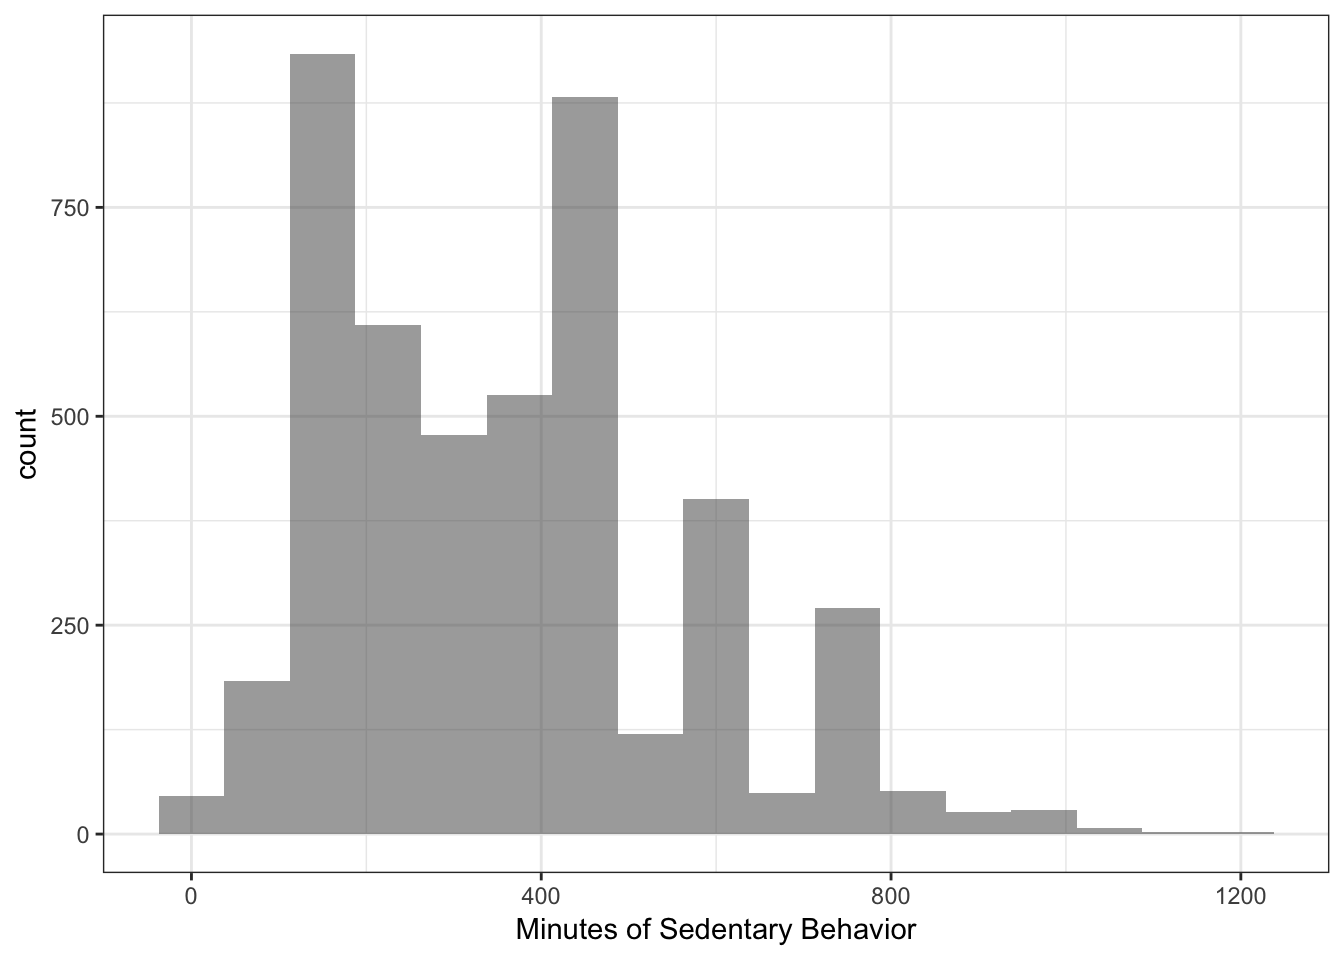
\includegraphics{_main_files/figure-latex/unnamed-chunk-86-1} and so
other methods related to poisson may be necessary. For this book, we are
not going to be delving into these in depth but we will introduce some
below.

\subsection*{Gamma}\label{gamma}
\addcontentsline{toc}{subsection}{Gamma}

Regression with a gamma distribution are often found when analyzing
costs in dollars. It is very similar to poisson but does not require
integers and can handle more dispersion. However, the outcome must have
values \(> 0\). Just for demonstration:

\begin{Shaded}
\begin{Highlighting}[]
\NormalTok{## Adjust sed}
\NormalTok{df}\OperatorTok{$}\NormalTok{sed_gamma <-}\StringTok{ }\NormalTok{df}\OperatorTok{$}\NormalTok{sed }\OperatorTok{+}\StringTok{ }\FloatTok{0.01}
\NormalTok{g_fit <-}\StringTok{ }\KeywordTok{glm}\NormalTok{(sed_gamma }\OperatorTok{~}\StringTok{ }\NormalTok{asthma }\OperatorTok{+}\StringTok{ }\NormalTok{race }\OperatorTok{+}\StringTok{ }\NormalTok{famsize, }
    \DataTypeTok{data =}\NormalTok{ df, }\DataTypeTok{family =} \StringTok{"Gamma"}\NormalTok{)}
\KeywordTok{summary}\NormalTok{(g_fit)}
\end{Highlighting}
\end{Shaded}

\begin{verbatim}
## 
## Call:
## glm(formula = sed_gamma ~ asthma + race + famsize, family = "Gamma", 
##     data = df)
## 
## Deviance Residuals: 
##    Min      1Q  Median      3Q     Max  
## -4.359  -0.461  -0.084   0.293   1.687  
## 
## Coefficients:
##                    Estimate Std. Error
## (Intercept)        3.57e-03   1.13e-04
## asthma            -1.60e-04   5.86e-05
## raceOtherHispanic -4.87e-04   1.31e-04
## raceWhite         -1.09e-03   1.08e-04
## raceBlack         -1.07e-03   1.10e-04
## raceOther         -1.11e-03   1.15e-04
## famsize            5.11e-05   1.55e-05
##                   t value Pr(>|t|)    
## (Intercept)         31.51   <2e-16 ***
## asthma              -2.74   0.0063 ** 
## raceOtherHispanic   -3.72   0.0002 ***
## raceWhite          -10.11   <2e-16 ***
## raceBlack           -9.70   <2e-16 ***
## raceOther           -9.70   <2e-16 ***
## famsize              3.29   0.0010 ** 
## ---
## Signif. codes:  
##   0 '***' 0.001 '**' 0.01 '*' 0.05 '.' 0.1  ' ' 1
## 
## (Dispersion parameter for Gamma family taken to be 0.293)
## 
##     Null deviance: 1664.8  on 4436  degrees of freedom
## Residual deviance: 1604.2  on 4430  degrees of freedom
##   (195 observations deleted due to missingness)
## AIC: 59154
## 
## Number of Fisher Scoring iterations: 5
\end{verbatim}

\subsection*{Two-Part or Hurdle Models}\label{two-part-or-hurdle-models}
\addcontentsline{toc}{subsection}{Two-Part or Hurdle Models}

We are going to use the \texttt{pscl} package to run a hurdle model.
These models are built for situations where there is a count variable
with many zeros (``zero-inflated''). The hurdle model makes slightly
different assumptions regarding the zeros than the pure negative
binomial that we present next. The hurdle consists of two models: one
for whether the person had a zero or more (binomial) and if more than
zero, how many (poisson).

To run a hurdle model, we are going to make a sedentary variable with
many more zeros to illustrate and then we will run a hurdle model.

\begin{Shaded}
\begin{Highlighting}[]
\NormalTok{## Zero inflated sedentary (don't worry too}
\NormalTok{## much about the specifics)}
\NormalTok{df}\OperatorTok{$}\NormalTok{sed_zero <-}\StringTok{ }\KeywordTok{ifelse}\NormalTok{(}\KeywordTok{sample}\NormalTok{(}\DecValTok{1}\OperatorTok{:}\DecValTok{100}\NormalTok{, }\DataTypeTok{size =} \KeywordTok{length}\NormalTok{(df}\OperatorTok{$}\NormalTok{sed), }
    \DataTypeTok{replace =} \OtherTok{TRUE}\NormalTok{) }\OperatorTok\StringTok{ }\KeywordTok{c}\NormalTok{(}\DecValTok{5}\NormalTok{, }\DecValTok{10}\NormalTok{, }\DecValTok{11}\NormalTok{, }\DecValTok{20}\OperatorTok{:}\DecValTok{25}\NormalTok{), }
    \DecValTok{0}\NormalTok{, df}\OperatorTok{$}\NormalTok{sed)}
\NormalTok{## Hurdle model}
\KeywordTok{library}\NormalTok{(pscl)}
\NormalTok{h_fit =}\StringTok{ }\KeywordTok{hurdle}\NormalTok{(sed_zero }\OperatorTok{~}\StringTok{ }\NormalTok{asthma }\OperatorTok{+}\StringTok{ }\NormalTok{race }\OperatorTok{+}\StringTok{ }\NormalTok{famsize, }
    \DataTypeTok{data =}\NormalTok{ df)}
\KeywordTok{summary}\NormalTok{(h_fit)}
\end{Highlighting}
\end{Shaded}

\begin{verbatim}
## 
## Call:
## hurdle(formula = sed_zero ~ asthma + race + 
##     famsize, data = df)
## 
## Pearson residuals:
##    Min     1Q Median     3Q    Max 
## -3.343 -1.477 -0.268  1.270  9.406 
## 
## Count model coefficients (truncated poisson with log link):
##                    Estimate Std. Error
## (Intercept)        5.657684   0.003745
## asthma             0.054472   0.002281
## raceOtherHispanic  0.140883   0.004311
## raceWhite          0.347588   0.003525
## raceBlack          0.346079   0.003623
## raceOther          0.356534   0.003822
## famsize           -0.021580   0.000576
##                   z value Pr(>|z|)    
## (Intercept)        1510.9   <2e-16 ***
## asthma               23.9   <2e-16 ***
## raceOtherHispanic    32.7   <2e-16 ***
## raceWhite            98.6   <2e-16 ***
## raceBlack            95.5   <2e-16 ***
## raceOther            93.3   <2e-16 ***
## famsize             -37.4   <2e-16 ***
## Zero hurdle model coefficients (binomial with logit link):
##                    Estimate Std. Error
## (Intercept)        2.24e+00   2.06e-01
## asthma            -3.13e-01   1.33e-01
## raceOtherHispanic  6.23e-02   2.35e-01
## raceWhite          2.87e-03   1.89e-01
## raceBlack          2.04e-01   2.01e-01
## raceOther          7.37e-02   2.13e-01
## famsize           -3.94e-05   3.58e-02
##                   z value Pr(>|z|)    
## (Intercept)         10.89   <2e-16 ***
## asthma              -2.35    0.019 *  
## raceOtherHispanic    0.27    0.790    
## raceWhite            0.02    0.988    
## raceBlack            1.02    0.309    
## raceOther            0.35    0.730    
## famsize              0.00    0.999    
## ---
## Signif. codes:  0 '***' 0.001 '**' 0.01 '*' 0.05 '.' 0.1 ' ' 1 
## 
## Number of iterations in BFGS optimization: 12 
## Log-likelihood: -2.3e+05 on 14 Df
\end{verbatim}

Notice that the output has two parts: ``Count model coefficients
(truncated poisson with log link):'' and ``Zero hurdle model
coefficients (binomial with logit link):''. Together they tell us about
the relationship between the predictors and a count variable with many
zeros.

\subsection*{Negative Binomial}\label{negative-binomial}
\addcontentsline{toc}{subsection}{Negative Binomial}

Similar to that above, negative binomial is for zero-inflated count
variables. It makes slightly different assumptions than the hurdle and
doesn't use a two-part approach. In order to run a negative binomial
model we'll use the \texttt{MASS} package and the \texttt{glm.nb()}
function.

\begin{Shaded}
\begin{Highlighting}[]
\KeywordTok{library}\NormalTok{(MASS)}
\NormalTok{fit_nb <-}\StringTok{ }\KeywordTok{glm.nb}\NormalTok{(sed_zero }\OperatorTok{~}\StringTok{ }\NormalTok{asthma }\OperatorTok{+}\StringTok{ }\NormalTok{race }\OperatorTok{+}\StringTok{ }\NormalTok{famsize, }
    \DataTypeTok{data =}\NormalTok{ df)}
\KeywordTok{summary}\NormalTok{(fit_nb)}
\end{Highlighting}
\end{Shaded}

Note that this model is not really appropriate because our data is
somewhat contrived.

\section*{Beta Regression}\label{beta-regression}
\addcontentsline{toc}{section}{Beta Regression}

For outcomes that are bound between a lower and upper bound, Beta
Regression is a great method. For example, if we are looking at test
scores that are bound between 0 and 100. It is a very flexible method
and allows for some extra analysis regarding the variation.

For this, we are going to use the \texttt{betareg} package. But first,
we are going to reach a little and create a ficticiously bound variable
in the data set.

\begin{Shaded}
\begin{Highlighting}[]
\NormalTok{## Variable bound between 0 and 1}
\NormalTok{df}\OperatorTok{$}\NormalTok{beta_var <-}\StringTok{ }\KeywordTok{sample}\NormalTok{(}\KeywordTok{seq}\NormalTok{(}\FloatTok{0.05}\NormalTok{, }\FloatTok{0.99}\NormalTok{, }\DataTypeTok{by =} \FloatTok{0.01}\NormalTok{), }
    \DataTypeTok{size =} \KeywordTok{length}\NormalTok{(df}\OperatorTok{$}\NormalTok{asthma), }\DataTypeTok{replace =} \OtherTok{TRUE}\NormalTok{)}
\KeywordTok{library}\NormalTok{(betareg)}
\NormalTok{fit_beta <-}\StringTok{ }\KeywordTok{betareg}\NormalTok{(beta_var }\OperatorTok{~}\StringTok{ }\NormalTok{asthma }\OperatorTok{+}\StringTok{ }\NormalTok{race }\OperatorTok{+}\StringTok{ }
\StringTok{    }\NormalTok{famsize, }\DataTypeTok{data =}\NormalTok{ df)}
\KeywordTok{summary}\NormalTok{(fit_beta)}
\end{Highlighting}
\end{Shaded}

\begin{verbatim}
## 
## Call:
## betareg(formula = beta_var ~ asthma + race + 
##     famsize, data = df)
## 
## Standardized weighted residuals 2:
##    Min     1Q Median     3Q    Max 
## -2.034 -0.710 -0.037  0.623  2.850 
## 
## Coefficients (mean model with logit link):
##                   Estimate Std. Error
## (Intercept)         0.0471     0.0634
## asthma              0.0645     0.0438
## raceOtherHispanic   0.0241     0.0722
## raceWhite           0.0324     0.0589
## raceBlack           0.0458     0.0611
## raceOther           0.0334     0.0655
## famsize             0.0109     0.0108
##                   z value Pr(>|z|)
## (Intercept)          0.74     0.46
## asthma               1.47     0.14
## raceOtherHispanic    0.33     0.74
## raceWhite            0.55     0.58
## raceBlack            0.75     0.45
## raceOther            0.51     0.61
## famsize              1.01     0.31
## 
## Phi coefficients (precision model with identity link):
##       Estimate Std. Error z value Pr(>|z|)
## (phi)   2.4495     0.0446      55   <2e-16
##          
## (phi) ***
## ---
## Signif. codes:  0 '***' 0.001 '**' 0.01 '*' 0.05 '.' 0.1 ' ' 1 
## 
## Type of estimator: ML (maximum likelihood)
## Log-likelihood:   82 on 8 Df
## Pseudo R-squared: 0.000871
## Number of iterations: 18 (BFGS) + 2 (Fisher scoring)
\end{verbatim}

The output provides coefficients and the ``Phi'' coefficients. Both are
important parts of using beta regression but we are not going to discuss
it here.

There are many resources available to learn more about beta regression
and each of these GLM's. As for now, we are going to move on to more
complex modeling where there are clustering or repeated measures in the
data.

\section*{Conclusions}\label{conclusions-1}
\addcontentsline{toc}{section}{Conclusions}

One of the great things about \texttt{R} is that most modeling is very
similar to the basic \texttt{lm()} function. In all of these GLM's the
arguments are nearly all the same: a formula, the data, and family of
model. As you'll see for Multilevel and Other Models chapters, this does
not change much. Having a good start with basic models and GLM's gets
you ready for nearly every other modeling type in \texttt{R}.

\chapter*{Chapter 6: Multilevel
Modeling}\label{chapter-6-multilevel-modeling}
\addcontentsline{toc}{chapter}{Chapter 6: Multilevel Modeling}

\begin{quote}
``Simplicity does not precede complexity, but follows it.''

--- Alan Perlis
\end{quote}

Multilevel data are more complex and don't meet the assumptions of
regular linear or generalized linear models. But with the right modeling
schemes, the results can be very interpretable and actionable. Two
powerful forms of multilevel modeling are:

\begin{enumerate}
\def\labelenumi{\arabic{enumi}.}
\tightlist
\item
  Generalized Estimating Equations (GEE)
\item
  Mixed effects (ME; i.e., hierarchical linear modeling, multilevel
  modeling)
\end{enumerate}

Several similarities and differences should be noted briefly. As for
similarities, they both attempt to control for the lack of independence
within clusters, although they do it in different ways. Also, they are
both built on linear regression which makes them flexible and powerful
at finding relationships in the data.

The differences are subtle but important. First, the interpretation is
somewhat different between the two. GEE is a population-averaged (e.g.,
marginal) model whereas ME is subject specific. In other words,
\emph{GEE is the average effect} while \emph{ME is the effect found in
the average person}. In a linear model, these coefficients are the same
but when we use different forms such as logistic or poisson, these can
be quite different (although in my experience they generally tell a
similar story). Second, ME models are much more complex than the GEE
models and can struggle with convergence compared to the GEE. This also
means that GEE's are generally fitted much more quickly. Still the
choice of the modeling technique should be driven by your hypotheses and
not totally dependent on speed of the computation.

First, if we needed to, we'd reshape our data so that it is ready for
the analyses (see Chapter 8 for more on reshaping). For both modeling
techniques we want our data in long form\footnote{We discuss what this
  means in much more depth and demonstrate reshaping of data in Chapter
  8. It is an important tool to understand if you are working with data
  in various forms. Although many reshape their data by
  copying-and-pasting in a spreadsheet, what we present in Chapter 8 is
  much more efficient, cleaner, less error-prone, and replicatable.}.
What this implies is that each row is an observation. What this actually
means about the data depends on the data. For example, if you have
repeated measures, then often data is stored in wide form---a row is an
individual. To make this long, we want each time point within a person
to be a row---a single individual can have multiple rows but each row is
a unique observation.

Currently, our data is in long form since we are working within
community clusters within this data. So, each row is an observation and
each cluster has multiple rows. Note that although these analyses will
be within community clusters instead of within subjects (i.e.~repeated
measures), the overall steps will be the exact same.

This chapter certainly does not cover all of multilevel modeling in
\texttt{R}. Entire books are dedicated to that single subject. Rather,
we are introducing the methods and the packages that can be used to
start using these methods.

\section*{GEE}\label{gee}
\addcontentsline{toc}{section}{GEE}

There are two packages, intimately related, that allow us to perform GEE
modeling---\texttt{gee} and \texttt{geepack}. These have some great
features and make running a fairly complex model pretty simple. However,
as great as they are, there are some annoying shortcomings. We'll get to
a few of them throughout this section.

GEE's, in general, want a few pieces of information from you. First, the
outcome and predictors. This is just as in linear regression and GLM's.
Second, we need to provide a correlation structure. This tells the model
the approximate pattern of correlations between the time points or
clusters. It also wants a variable that tells the cluster ID's. Finally,
it also wants the family (i.e.~the type of distribution).

Since this is not longitudinal, but rather clustered within communities,
we'll assume for this analysis an unstructured correlation structure. It
is the most flexible and we have enough power for it here.

For \texttt{geepack} to work, we need to filter out the missing values
for the variables that will be in the model.

\begin{Shaded}
\begin{Highlighting}[]
\NormalTok{df2 <-}\StringTok{ }\NormalTok{df }\OperatorTok\StringTok{ }\KeywordTok{filter}\NormalTok{(}\KeywordTok{complete.cases}\NormalTok{(dep, famsize, }
\NormalTok{    sed, race, asthma))}
\end{Highlighting}
\end{Shaded}

Now, we'll build the model with both packages (just for demonstration).
We predict depression with asthma, family size, minutes of sedentary
behavior, and the subject's race.

\begin{Shaded}
\begin{Highlighting}[]
\KeywordTok{library}\NormalTok{(gee)}
\NormalTok{fit_gee <-}\StringTok{ }\KeywordTok{gee}\NormalTok{(dep }\OperatorTok{~}\StringTok{ }\NormalTok{asthma }\OperatorTok{+}\StringTok{ }\NormalTok{famsize }\OperatorTok{+}\StringTok{ }\NormalTok{sed }\OperatorTok{+}\StringTok{ }
\StringTok{    }\NormalTok{race, }\DataTypeTok{data =}\NormalTok{ df2, }\DataTypeTok{id =}\NormalTok{ df2}\OperatorTok{$}\NormalTok{sdmvstra, }\DataTypeTok{corstr =} \StringTok{"unstructured"}\NormalTok{)}
\end{Highlighting}
\end{Shaded}

\begin{verbatim}
##       (Intercept)      asthmaAsthma 
##           2.50002           1.35608 
##           famsize               sed 
##          -0.04213           0.00136 
## raceOtherHispanic         raceWhite 
##           1.18500           0.11395 
##         raceBlack         raceOther 
##           0.10054          -0.55548
\end{verbatim}

\begin{Shaded}
\begin{Highlighting}[]
\KeywordTok{summary}\NormalTok{(fit_gee)}\OperatorTok{$}\NormalTok{coef}
\end{Highlighting}
\end{Shaded}

\begin{verbatim}
##                   Estimate Naive S.E.
## (Intercept)        2.49551   0.286782
## asthmaAsthma       1.35304   0.186710
## famsize           -0.03949   0.046195
## sed                0.00136   0.000336
## raceOtherHispanic  1.19248   0.307556
## raceWhite          0.11619   0.253155
## raceBlack          0.09680   0.262583
## raceOther         -0.55505   0.280930
##                   Naive z Robust S.E.
## (Intercept)         8.702    0.269043
## asthmaAsthma        7.247    0.213798
## famsize            -0.855    0.045747
## sed                 4.039    0.000355
## raceOtherHispanic   3.877    0.330961
## raceWhite           0.459    0.227969
## raceBlack           0.369    0.236050
## raceOther          -1.976    0.240657
##                   Robust z
## (Intercept)          9.276
## asthmaAsthma         6.329
## famsize             -0.863
## sed                  3.823
## raceOtherHispanic    3.603
## raceWhite            0.510
## raceBlack            0.410
## raceOther           -2.306
\end{verbatim}

\begin{Shaded}
\begin{Highlighting}[]
\KeywordTok{library}\NormalTok{(geepack)}
\NormalTok{fit_geeglm <-}\StringTok{ }\KeywordTok{geeglm}\NormalTok{(dep }\OperatorTok{~}\StringTok{ }\NormalTok{asthma }\OperatorTok{+}\StringTok{ }\NormalTok{famsize }\OperatorTok{+}\StringTok{ }
\StringTok{    }\NormalTok{sed }\OperatorTok{+}\StringTok{ }\NormalTok{race, }\DataTypeTok{data =}\NormalTok{ df2, }\DataTypeTok{id =}\NormalTok{ df2}\OperatorTok{$}\NormalTok{sdmvstra, }
    \DataTypeTok{corstr =} \StringTok{"unstructured"}\NormalTok{)}
\KeywordTok{summary}\NormalTok{(fit_geeglm)}
\end{Highlighting}
\end{Shaded}

\begin{verbatim}
## 
## Call:
## geeglm(formula = dep ~ asthma + famsize + sed + race, data = df2, 
##     id = df2$sdmvstra, corstr = "unstructured")
## 
##  Coefficients:
##                    Estimate   Std.err  Wald
## (Intercept)        2.557936  0.270072 89.71
## asthmaAsthma       1.349289  0.215620 39.16
## famsize           -0.044672  0.045709  0.96
## sed                0.001301  0.000355 13.45
## raceOtherHispanic  1.175037  0.331898 12.53
## raceWhite          0.080638  0.229566  0.12
## raceBlack          0.064203  0.236326  0.07
## raceOther         -0.590205  0.241338  5.98
##                   Pr(>|W|)    
## (Intercept)        < 2e-16 ***
## asthmaAsthma       3.9e-10 ***
## famsize            0.32841    
## sed                0.00024 ***
## raceOtherHispanic  0.00040 ***
## raceWhite          0.72539    
## raceBlack          0.78587    
## raceOther          0.01446 *  
## ---
## Signif. codes:  
##   0 '***' 0.001 '**' 0.01 '*' 0.05 '.' 0.1  ' ' 1
## 
## Estimated Scale Parameters:
##             Estimate Std.err
## (Intercept)     19.5   0.784
## 
## Correlation: Structure = unstructured  Link = identity 
## 
## Estimated Correlation Parameters:
##           Estimate Std.err
## alpha.1:2   0.1248  0.0165
## alpha.1:3   0.4207  0.1034
## alpha.1:4   2.8964  1.0668
## alpha.1:5  -1.8545  0.2028
## alpha.2:3   0.1224  0.0633
## alpha.2:4  -0.0894  0.2023
## alpha.2:5   0.2054  0.0372
## alpha.3:4  -0.4960  0.1123
## alpha.3:5   0.2504  0.0388
## alpha.4:5  -0.6694  0.0876
## Number of clusters:   4109   Maximum cluster size: 5
\end{verbatim}

The \texttt{gee} package doesn't directly provide p-values but provides
the z-scores, which can be used to find the p-values. The
\texttt{geepack} provides the p-values in the way you'll see in the
\texttt{lm()} and \texttt{glm()} functions.

These models are interpreted just as the regular GLM. It has adjusted
for the correlations within the clusters and provides valid standard
errors and p-values.

\section*{Mixed Effects}\label{mixed-effects}
\addcontentsline{toc}{section}{Mixed Effects}

Mixed effects models require a bit more thinking about the effects. It
is called ``mixed effects'' because we include both fixed and random
effects into the model simultaneously. The random effects are those that
we don't necessarily care about the specific values but want to control
for it and/or estimate the variance. The fixed effects are those we are
used to estimating in linear models and GLM's.

These are a bit more clear with an example. We will do the same overall
model as we did with the GEE but we'll use ME. To do so, we'll use the
\texttt{lme4} package. In the model below, we predict depression with
asthma, family size, minutes of sedentary behavior, and the subject's
race. We have a random intercept (which allows the intercept to vary
across clusters).

\begin{Shaded}
\begin{Highlighting}[]
\KeywordTok{library}\NormalTok{(lme4)}
\NormalTok{fit_me <-}\StringTok{ }\KeywordTok{lmer}\NormalTok{(dep }\OperatorTok{~}\StringTok{ }\NormalTok{asthma }\OperatorTok{+}\StringTok{ }\NormalTok{famsize }\OperatorTok{+}\StringTok{ }\NormalTok{sed }\OperatorTok{+}\StringTok{ }
\StringTok{    }\NormalTok{race }\OperatorTok{+}\StringTok{ }\NormalTok{(}\DecValTok{1} \OperatorTok{|}\StringTok{ }\NormalTok{cluster), }\DataTypeTok{data =}\NormalTok{ df2, }\DataTypeTok{REML =} \OtherTok{FALSE}\NormalTok{)}
\KeywordTok{summary}\NormalTok{(fit_me)}
\end{Highlighting}
\end{Shaded}

\begin{verbatim}
## Linear mixed model fit by maximum  likelihood
##  [lmerMod]
## Formula: 
## dep ~ asthma + famsize + sed + race + (1 | cluster)
##    Data: df2
## 
##      AIC      BIC   logLik deviance df.resid 
##    25780    25844   -12880    25760     4427 
## 
## Scaled residuals: 
##    Min     1Q Median     3Q    Max 
## -1.327 -0.635 -0.355  0.272  5.435 
## 
## Random effects:
##  Groups   Name        Variance Std.Dev.
##  cluster  (Intercept)  0.105   0.324   
##  Residual             19.389   4.403   
## Number of obs: 4437, groups:  cluster, 14
## 
## Fixed effects:
##                    Estimate Std. Error
## (Intercept)        2.491678   0.302768
## asthmaAsthma       1.335445   0.186618
## famsize           -0.042857   0.046341
## sed                0.001425   0.000337
## raceOtherHispanic  1.289890   0.320595
## raceWhite          0.008348   0.259449
## raceBlack          0.171658   0.273382
## raceOther         -0.552746   0.285512
##                   t value
## (Intercept)          8.23
## asthmaAsthma         7.16
## famsize             -0.92
## sed                  4.23
## raceOtherHispanic    4.02
## raceWhite            0.03
## raceBlack            0.63
## raceOther           -1.94
## 
## Correlation of Fixed Effects:
##             (Intr) asthmA famsiz sed   
## asthmaAsthm -0.042                     
## famsize     -0.510 -0.004              
## sed         -0.324 -0.044  0.051       
## rcOthrHspnc -0.556 -0.032  0.051 -0.038
## raceWhite   -0.680 -0.038  0.135 -0.148
## raceBlack   -0.643 -0.057  0.094 -0.131
## raceOther   -0.580  0.000  0.048 -0.135
##             rcOthH racWht rcBlck
## asthmaAsthm                     
## famsize                         
## sed                             
## rcOthrHspnc                     
## raceWhite    0.639              
## raceBlack    0.624  0.775       
## raceOther    0.589  0.725  0.693
\end{verbatim}

You'll see that there are no p-values provided here. This is because
p-values are not well-defined in the ME framework. A good way to test it
can be through the \texttt{anova()} function, comparing models. Let's
compare a model with and without \texttt{asthma} to see if the model is
significantly better with it in.

\begin{Shaded}
\begin{Highlighting}[]
\NormalTok{fit_me1 <-}\StringTok{ }\KeywordTok{lmer}\NormalTok{(dep }\OperatorTok{~}\StringTok{ }\NormalTok{famsize }\OperatorTok{+}\StringTok{ }\NormalTok{sed }\OperatorTok{+}\StringTok{ }\NormalTok{race }\OperatorTok{+}\StringTok{ }\NormalTok{(}\DecValTok{1} \OperatorTok{|}\StringTok{ }
\StringTok{    }\NormalTok{cluster), }\DataTypeTok{data =}\NormalTok{ df2, }\DataTypeTok{REML =} \OtherTok{FALSE}\NormalTok{)}

\KeywordTok{anova}\NormalTok{(fit_me, fit_me1)}
\end{Highlighting}
\end{Shaded}

\begin{verbatim}
## Data: df2
## Models:
## fit_me1: dep ~ famsize + sed + race + (1 | cluster)
## fit_me: dep ~ asthma + famsize + sed + race + (1 | cluster)
##         Df   AIC   BIC logLik deviance Chisq
## fit_me1  9 25829 25886 -12905    25811      
## fit_me  10 25780 25844 -12880    25760  50.9
##         Chi Df Pr(>Chisq)    
## fit_me1                      
## fit_me       1    9.9e-13 ***
## ---
## Signif. codes:  
##   0 '***' 0.001 '**' 0.01 '*' 0.05 '.' 0.1  ' ' 1
\end{verbatim}

This comparison strongly suggests that \texttt{asthma} is a significant
predictor (\(\chi^2 = 50.5\), p \textless{} .001). We can do this with
both fixed and random effects, as below:

\begin{Shaded}
\begin{Highlighting}[]
\NormalTok{fit_me2 <-}\StringTok{ }\KeywordTok{lmer}\NormalTok{(dep }\OperatorTok{~}\StringTok{ }\NormalTok{famsize }\OperatorTok{+}\StringTok{ }\NormalTok{sed }\OperatorTok{+}\StringTok{ }\NormalTok{race }\OperatorTok{+}\StringTok{ }\NormalTok{(}\DecValTok{1} \OperatorTok{|}\StringTok{ }
\StringTok{    }\NormalTok{cluster), }\DataTypeTok{data =}\NormalTok{ df2, }\DataTypeTok{REML =} \OtherTok{TRUE}\NormalTok{)}
\NormalTok{fit_me3 <-}\StringTok{ }\KeywordTok{lmer}\NormalTok{(dep }\OperatorTok{~}\StringTok{ }\NormalTok{famsize }\OperatorTok{+}\StringTok{ }\NormalTok{sed }\OperatorTok{+}\StringTok{ }\NormalTok{race }\OperatorTok{+}\StringTok{ }\NormalTok{(}\DecValTok{1} \OperatorTok{+}\StringTok{ }
\StringTok{    }\NormalTok{asthma }\OperatorTok{|}\StringTok{ }\NormalTok{cluster), }\DataTypeTok{data =}\NormalTok{ df2, }\DataTypeTok{REML =} \OtherTok{TRUE}\NormalTok{)}
\KeywordTok{anova}\NormalTok{(fit_me2, fit_me3, }\DataTypeTok{refit =} \OtherTok{FALSE}\NormalTok{)}
\end{Highlighting}
\end{Shaded}

\begin{verbatim}
## Data: df2
## Models:
## fit_me2: dep ~ famsize + sed + race + (1 | cluster)
## fit_me3: dep ~ famsize + sed + race + (1 + asthma | cluster)
##         Df   AIC   BIC logLik deviance Chisq
## fit_me2  9 25855 25912 -12918    25837      
## fit_me3 11 25821 25892 -12900    25799  37.3
##         Chi Df Pr(>Chisq)    
## fit_me2                      
## fit_me3      2      8e-09 ***
## ---
## Signif. codes:  
##   0 '***' 0.001 '**' 0.01 '*' 0.05 '.' 0.1  ' ' 1
\end{verbatim}

Here, including random slopes for asthma appears to be significant
(\(\chi^2 = 36.9\), p \textless{} .001).

Linear mixed effects models converge pretty well. You'll see that the
conclusions and estimates are very similar to that of the GEE. For
generalized versions of ME, the convergence can be harder and more
picky. As we'll see below, it complains about large eigenvalues and
tells us to rescale some of the variables.

\begin{Shaded}
\begin{Highlighting}[]
\KeywordTok{library}\NormalTok{(lme4)}
\NormalTok{fit_gme <-}\StringTok{ }\KeywordTok{glmer}\NormalTok{(dep2 }\OperatorTok{~}\StringTok{ }\NormalTok{asthma }\OperatorTok{+}\StringTok{ }\NormalTok{famsize }\OperatorTok{+}\StringTok{ }\NormalTok{sed }\OperatorTok{+}\StringTok{ }
\StringTok{    }\NormalTok{race }\OperatorTok{+}\StringTok{ }\NormalTok{(}\DecValTok{1} \OperatorTok{|}\StringTok{ }\NormalTok{cluster), }\DataTypeTok{data =}\NormalTok{ df2, }\DataTypeTok{family =} \StringTok{"binomial"}\NormalTok{)}
\end{Highlighting}
\end{Shaded}

\begin{verbatim}
## Warning in checkConv(attr(opt, "derivs"),
## opt$par, ctrl = control$checkConv, :
## Model failed to converge with max|grad| =
## 0.00854237 (tol = 0.001, component 1)
\end{verbatim}

\begin{verbatim}
## Warning in checkConv(attr(opt, "derivs"), opt$par, ctrl = control$checkConv, : Model is nearly unidentifiable: very large eigenvalue
##  - Rescale variables?;Model is nearly unidentifiable: large eigenvalue ratio
##  - Rescale variables?
\end{verbatim}

After a quick check, we can see that \texttt{sed} is huge compared to
the other variables. If we simply rescale it, using the \texttt{I()}
function within the model formula, we can rescale it by 1,000. Here,
that is all it needed to converge.

\begin{Shaded}
\begin{Highlighting}[]
\KeywordTok{library}\NormalTok{(lme4)}
\NormalTok{fit_gme <-}\StringTok{ }\KeywordTok{glmer}\NormalTok{(dep2 }\OperatorTok{~}\StringTok{ }\NormalTok{asthma }\OperatorTok{+}\StringTok{ }\NormalTok{famsize }\OperatorTok{+}\StringTok{ }\KeywordTok{I}\NormalTok{(sed}\OperatorTok{/}\DecValTok{1000}\NormalTok{) }\OperatorTok{+}\StringTok{ }
\StringTok{    }\NormalTok{race }\OperatorTok{+}\StringTok{ }\NormalTok{(}\DecValTok{1} \OperatorTok{|}\StringTok{ }\NormalTok{cluster), }\DataTypeTok{data =}\NormalTok{ df2, }\DataTypeTok{family =} \StringTok{"binomial"}\NormalTok{)}
\KeywordTok{summary}\NormalTok{(fit_gme)}
\end{Highlighting}
\end{Shaded}

\begin{verbatim}
## Generalized linear mixed model fit by
##   maximum likelihood (Laplace  Approximation)
##  [glmerMod]
##  Family: binomial  ( logit )
## Formula: 
## dep2 ~ asthma + famsize + I(sed/1000) + race + (1 | cluster)
##    Data: df2
## 
##      AIC      BIC   logLik deviance df.resid 
##     2665     2722    -1323     2647     4428 
## 
## Scaled residuals: 
##    Min     1Q Median     3Q    Max 
## -0.635 -0.329 -0.295 -0.258  5.032 
## 
## Random effects:
##  Groups  Name        Variance Std.Dev.
##  cluster (Intercept) 0.0232   0.152   
## Number of obs: 4437, groups:  cluster, 14
## 
## Fixed effects:
##                   Estimate Std. Error
## (Intercept)        -2.6316     0.2435
## asthmaAsthma        0.5619     0.1281
## famsize            -0.0336     0.0374
## I(sed/1000)         0.5835     0.2618
## raceOtherHispanic   0.7564     0.2421
## raceWhite           0.0955     0.2159
## raceBlack           0.0531     0.2277
## raceOther          -0.4950     0.2591
##                   z value Pr(>|z|)    
## (Intercept)        -10.81  < 2e-16 ***
## asthmaAsthma         4.39  1.2e-05 ***
## famsize             -0.90   0.3696    
## I(sed/1000)          2.23   0.0258 *  
## raceOtherHispanic    3.12   0.0018 ** 
## raceWhite            0.44   0.6581    
## raceBlack            0.23   0.8155    
## raceOther           -1.91   0.0560 .  
## ---
## Signif. codes:  
##   0 '***' 0.001 '**' 0.01 '*' 0.05 '.' 0.1  ' ' 1
## 
## Correlation of Fixed Effects:
##             (Intr) asthmA famsiz I(/100
## asthmaAsthm -0.057                     
## famsize     -0.491 -0.012              
## I(sed/1000) -0.324 -0.042  0.031       
## rcOthrHspnc -0.653 -0.031  0.044 -0.029
## raceWhite   -0.715 -0.037  0.132 -0.148
## raceBlack   -0.684 -0.064  0.088 -0.124
## raceOther   -0.571 -0.003  0.046 -0.122
##             rcOthH racWht rcBlck
## asthmaAsthm                     
## famsize                         
## I(sed/1000)                     
## rcOthrHspnc                     
## raceWhite    0.709              
## raceBlack    0.715  0.781       
## raceOther    0.606  0.688  0.653
\end{verbatim}

\section*{Conclusions}\label{conclusions-2}
\addcontentsline{toc}{section}{Conclusions}

This has been a really brief introduction into a thriving, large field
of statistical analyses. These are the general methods for using
\texttt{R} to analyze multilevel data. Our next chapter will discuss
more modeling techniques in \texttt{R}, including mediation, mixture,
and structural equation modeling.

\chapter*{Chapter 7: Other Modeling
Techniques}\label{chapter-7-other-modeling-techniques}
\addcontentsline{toc}{chapter}{Chapter 7: Other Modeling Techniques}

\begin{quote}
``Simplicity is the ultimate sophistication.''

--- Leonardo da Vinci
\end{quote}

In this chapter we cover, however briefly, modeling techniques that are
especially useful to make complex relationships easier to interpret. We
will focus on mediation and moderation modeling, methods relating to
structural equation modeling (SEM), and methods applicable to our field
from machine learning. Although these machine learning may appear very
different than mediation and SEM, they each have advantages that can
help in different situations. For example, SEM is useful when we know
there is a high degree of measurement error or our data has multiple
indicators for each construct. On the other hand, regularized regression
and random forests--two popular forms of machine learning--are great to
explore patterns and relationships there are hundreds or thousands of
variables that may predict an outcome.

Mediation modeling, although often used within SEM, can help us
understand pathways of effect from one variable to another. It is
especially useful with moderating variables (i.e., variables that
interact with another).

So we'll start with discussing mediation, then we'll move on to SEM,
followed by machine learning.

\section*{Mediation Modeling}\label{mediation-modeling}
\addcontentsline{toc}{section}{Mediation Modeling}

Mediation modeling can be done via several packages. For now, we
recommend using \texttt{lavaan} (stands for ``latent variable
analysis'')\footnote{The \texttt{lavaan} package has some great
  vignettes at \url{http://lavaan.ugent.be/} to help with the other
  types of models it can handle.}. Although it is technically still a
``beta'' version, it performs very well especially for more simple
models. It makes mediation modeling straightforward.

Below, we model the following mediation model: \[
depression = \beta_0 + \beta_1 asthma + \epsilon_1
\]

\[
time_{Sedentary} = \lambda_0 + \lambda_1 asthma + \lambda_2 depression + \epsilon_2
\]

In essence, we believe that asthma increases depression which in turn
increases the amount of time spent being sedentary.

\begin{Shaded}
\begin{Highlighting}[]
\KeywordTok{library}\NormalTok{(lavaan)}
\NormalTok{df}\OperatorTok{$}\NormalTok{sed_hr =}\StringTok{ }\NormalTok{df}\OperatorTok{$}\NormalTok{sed}\OperatorTok{/}\DecValTok{60}\NormalTok{  ## in hours instead of minutes}

\NormalTok{## Our model}
\NormalTok{model1 <-}\StringTok{ "}
\StringTok{  dep ~ asthma}
\StringTok{  sed_hr ~ dep + asthma}
\StringTok{"}
\NormalTok{## sem function to run the model}
\NormalTok{fit <-}\StringTok{ }\KeywordTok{sem}\NormalTok{(model1, }\DataTypeTok{data =}\NormalTok{ df)}
\KeywordTok{summary}\NormalTok{(fit)}
\end{Highlighting}
\end{Shaded}

\begin{verbatim}
## lavaan (0.5-23.1097) converged normally after  30 iterations
## 
##                                                   Used       Total
##   Number of observations                          4614        4632
## 
##   Estimator                                         ML
##   Minimum Function Test Statistic                0.000
##   Degrees of freedom                                 0
## 
## Parameter Estimates:
## 
##   Information                                 Expected
##   Standard Errors                             Standard
## 
## Regressions:
##                    Estimate  Std.Err
##   dep ~                             
##     asthma            1.478    0.183
##   sed_hr ~                          
##     dep               0.044    0.011
##     asthma            0.412    0.139
##   z-value  P(>|z|)
##                   
##     8.084    0.000
##                   
##     3.929    0.000
##     2.965    0.003
## 
## Variances:
##                    Estimate  Std.Err
##    .dep              19.597    0.408
##    .sed_hr           11.171    0.233
##   z-value  P(>|z|)
##    48.031    0.000
##    48.031    0.000
\end{verbatim}

From the output we see asthma does predict depression and depression
does predict time being sedentary. There is also a direct effect of
asthma on sedentary behavior even after controlling for depression. We
can further specify the model to have it give us the indirect effect and
direct effects tested.

\begin{Shaded}
\begin{Highlighting}[]
\NormalTok{## Our model}
\NormalTok{model2 <-}\StringTok{ "}
\StringTok{  dep ~ a*asthma}
\StringTok{  sed_hr ~ b*dep + c*asthma}
\StringTok{ }
\StringTok{  indirect := a*b}
\StringTok{  total := c + a*b}
\StringTok{"}
\NormalTok{## sem function to run the model}
\NormalTok{fit2 <-}\StringTok{ }\KeywordTok{sem}\NormalTok{(model2, }\DataTypeTok{data =}\NormalTok{ df)}
\KeywordTok{summary}\NormalTok{(fit2)}
\end{Highlighting}
\end{Shaded}

\begin{verbatim}
## lavaan (0.5-23.1097) converged normally after  30 iterations
## 
##                                                   Used       Total
##   Number of observations                          4614        4632
## 
##   Estimator                                         ML
##   Minimum Function Test Statistic                0.000
##   Degrees of freedom                                 0
## 
## Parameter Estimates:
## 
##   Information                                 Expected
##   Standard Errors                             Standard
## 
## Regressions:
##                    Estimate  Std.Err
##   dep ~                             
##     asthma     (a)    1.478    0.183
##   sed_hr ~                          
##     dep        (b)    0.044    0.011
##     asthma     (c)    0.412    0.139
##   z-value  P(>|z|)
##                   
##     8.084    0.000
##                   
##     3.929    0.000
##     2.965    0.003
## 
## Variances:
##                    Estimate  Std.Err
##    .dep              19.597    0.408
##    .sed_hr           11.171    0.233
##   z-value  P(>|z|)
##    48.031    0.000
##    48.031    0.000
## 
## Defined Parameters:
##                    Estimate  Std.Err
##     indirect          0.065    0.018
##     total             0.477    0.138
##   z-value  P(>|z|)
##     3.534    0.000
##     3.448    0.001
\end{verbatim}

We defined a few things in the model. First, we gave the coefficients
labels of \texttt{a}, \texttt{b}, and \texttt{c}. Doing so allows us to
define the \texttt{indirect} and \texttt{total} effects. Here we see the
indirect effect, although small, is significant at \(p < .001\). The
total effect is larger (not surprising) and is also significant.

Also note that we can make the regression equations have other
covariates as well if we needed to (i.e.~control for age or gender) just
as we do in regular regression.

\begin{Shaded}
\begin{Highlighting}[]
\NormalTok{## Our model}
\NormalTok{model2.}\DecValTok{1}\NormalTok{ <-}\StringTok{ "}
\StringTok{  dep ~ asthma + ridageyr}
\StringTok{  sed_hr ~ dep + asthma + ridageyr}
\StringTok{"}
\NormalTok{## sem function to run the model}
\NormalTok{fit2.}\DecValTok{1}\NormalTok{ <-}\StringTok{ }\KeywordTok{sem}\NormalTok{(model2.}\DecValTok{1}\NormalTok{, }\DataTypeTok{data =}\NormalTok{ df)}
\KeywordTok{summary}\NormalTok{(fit2.}\DecValTok{1}\NormalTok{)}
\end{Highlighting}
\end{Shaded}

\begin{verbatim}
## lavaan (0.5-23.1097) converged normally after  33 iterations
## 
##                                                   Used       Total
##   Number of observations                          4614        4632
## 
##   Estimator                                         ML
##   Minimum Function Test Statistic                0.000
##   Degrees of freedom                                 0
##   Minimum Function Value               0.0000000000000
## 
## Parameter Estimates:
## 
##   Information                                 Expected
##   Standard Errors                             Standard
## 
## Regressions:
##                    Estimate  Std.Err
##   dep ~                             
##     asthma            1.462    0.183
##     ridageyr         -0.005    0.004
##   sed_hr ~                          
##     dep               0.044    0.011
##     asthma            0.412    0.139
##     ridageyr         -0.000    0.003
##   z-value  P(>|z|)
##                   
##     7.980    0.000
##    -1.330    0.183
##                   
##     3.927    0.000
##     2.956    0.003
##    -0.063    0.950
## 
## Variances:
##                    Estimate  Std.Err
##    .dep              19.590    0.408
##    .sed_hr           11.171    0.233
##   z-value  P(>|z|)
##    48.031    0.000
##    48.031    0.000
\end{verbatim}

Although we don't show it here, we can also do moderation
(``interactions'') as part of the mediation model.

\section*{Structural Equation
Modeling}\label{structural-equation-modeling}
\addcontentsline{toc}{section}{Structural Equation Modeling}

Instead of summing our depression variable, we can use SEM to run the
mediation model from above but use the latent variable of depression
instead.

\begin{Shaded}
\begin{Highlighting}[]
\NormalTok{## Our model}
\NormalTok{model3 <-}\StringTok{ "}
\StringTok{  dep1 =~ dpq010 + dpq020 + dpq030 + dpq040 + dpq050 + dpq060 + dpq070 + dpq080 + dpq090}
\StringTok{  dep1 ~ a*asthma}
\StringTok{  sed_hr ~ b*dep1 + c*asthma}

\StringTok{  indirect := a*b}
\StringTok{  total := c + a*b}
\StringTok{"}
\NormalTok{## sem function to run the model}
\NormalTok{fit3 <-}\StringTok{ }\KeywordTok{sem}\NormalTok{(model3, }\DataTypeTok{data =}\NormalTok{ df)}
\KeywordTok{summary}\NormalTok{(fit3)}
\end{Highlighting}
\end{Shaded}

\begin{verbatim}
## lavaan (0.5-23.1097) converged normally after  47 iterations
## 
##                                                   Used       Total
##   Number of observations                          4614        4632
## 
##   Estimator                                         ML
##   Minimum Function Test Statistic             1065.848
##   Degrees of freedom                                43
##   P-value (Chi-square)                           0.000
## 
## Parameter Estimates:
## 
##   Information                                 Expected
##   Standard Errors                             Standard
## 
## Latent Variables:
##                    Estimate  Std.Err
##   dep1 =~                           
##     dpq010            1.000         
##     dpq020            1.096    0.024
##     dpq030            1.133    0.031
##     dpq040            1.149    0.030
##     dpq050            0.933    0.025
##     dpq060            0.929    0.022
##     dpq070            0.871    0.022
##     dpq080            0.686    0.019
##     dpq090            0.308    0.011
##   z-value  P(>|z|)
##                   
##                   
##    45.136    0.000
##    36.908    0.000
##    38.066    0.000
##    36.773    0.000
##    42.107    0.000
##    39.760    0.000
##    36.325    0.000
##    28.544    0.000
## 
## Regressions:
##                    Estimate  Std.Err
##   dep1 ~                            
##     asthma     (a)    0.173    0.023
##   sed_hr ~                          
##     dep1       (b)    0.342    0.105
##     asthma     (c)    0.418    0.139
##   z-value  P(>|z|)
##                   
##     7.656    0.000
##                   
##     3.275    0.001
##     2.998    0.003
## 
## Variances:
##                    Estimate  Std.Err
##    .dpq010            0.306    0.007
##    .dpq020            0.212    0.006
##    .dpq030            0.559    0.013
##    .dpq040            0.514    0.012
##    .dpq050            0.384    0.009
##    .dpq060            0.221    0.005
##    .dpq070            0.249    0.006
##    .dpq080            0.217    0.005
##    .dpq090            0.090    0.002
##    .sed_hr           11.179    0.233
##    .dep1              0.256    0.010
##   z-value  P(>|z|)
##    42.008    0.000
##    37.549    0.000
##    43.807    0.000
##    43.302    0.000
##    43.862    0.000
##    40.808    0.000
##    42.420    0.000
##    44.038    0.000
##    46.106    0.000
##    48.012    0.000
##    24.657    0.000
## 
## Defined Parameters:
##                    Estimate  Std.Err
##     indirect          0.059    0.020
##     total             0.477    0.138
##   z-value  P(>|z|)
##     3.019    0.003
##     3.448    0.001
\end{verbatim}

We defined \texttt{dep1} as a latent variable using
\texttt{=\textasciitilde{}}. Although the model does not fit the data
well--``\texttt{P-value\ (Chi-square)\ =\ 0.000}''--it is informative
for demonstration. We would likely need to find out how the measurement
model
(\texttt{dep1\ =\textasciitilde{}\ dpq010\ +\ dpq020\ +\ dpq030\ +})
actually fits before throwing it into a mediation model. We can do that
via:

\begin{Shaded}
\begin{Highlighting}[]
\NormalTok{model4 <-}\StringTok{ "}
\StringTok{  dep1 =~ dpq010 + dpq020 + dpq030 + dpq040 + dpq050 + dpq060 + dpq070 + dpq080 + dpq090}
\StringTok{"}
\NormalTok{fit4 <-}\StringTok{ }\KeywordTok{cfa}\NormalTok{(model4, }\DataTypeTok{data =}\NormalTok{ df)}
\KeywordTok{summary}\NormalTok{(fit4)}
\end{Highlighting}
\end{Shaded}

\begin{verbatim}
## lavaan (0.5-23.1097) converged normally after  29 iterations
## 
##   Number of observations                          4632
## 
##   Estimator                                         ML
##   Minimum Function Test Statistic              985.831
##   Degrees of freedom                                27
##   P-value (Chi-square)                           0.000
## 
## Parameter Estimates:
## 
##   Information                                 Expected
##   Standard Errors                             Standard
## 
## Latent Variables:
##                    Estimate  Std.Err
##   dep1 =~                           
##     dpq010            1.000         
##     dpq020            1.097    0.024
##     dpq030            1.128    0.031
##     dpq040            1.145    0.030
##     dpq050            0.927    0.025
##     dpq060            0.930    0.022
##     dpq070            0.870    0.022
##     dpq080            0.681    0.019
##     dpq090            0.307    0.011
##   z-value  P(>|z|)
##                   
##                   
##    45.383    0.000
##    36.962    0.000
##    38.136    0.000
##    36.630    0.000
##    42.294    0.000
##    39.941    0.000
##    36.350    0.000
##    28.609    0.000
## 
## Variances:
##                    Estimate  Std.Err
##    .dpq010            0.306    0.007
##    .dpq020            0.211    0.006
##    .dpq030            0.560    0.013
##    .dpq040            0.515    0.012
##    .dpq050            0.390    0.009
##    .dpq060            0.221    0.005
##    .dpq070            0.249    0.006
##    .dpq080            0.216    0.005
##    .dpq090            0.090    0.002
##     dep1              0.261    0.011
##   z-value  P(>|z|)
##    42.051    0.000
##    37.470    0.000
##    43.909    0.000
##    43.400    0.000
##    44.041    0.000
##    40.835    0.000
##    42.461    0.000
##    44.149    0.000
##    46.195    0.000
##    24.765    0.000
\end{verbatim}

As we can see, there is a lack of fit in the measurement model. It is
possible that these depression questions could be measuring more than
one factor. We could explore this using exploratory factor analysis. We
don't demonstrate that here, but know that it is possible to do in
\texttt{R} with a few other packages.

\section*{Machine Learning
Techniques}\label{machine-learning-techniques}
\addcontentsline{toc}{section}{Machine Learning Techniques}

We are briefly going to introduce some machine learning techniques that
may be of interest to researchers. We will quickly introduce and
demonstrate:

\begin{enumerate}
\def\labelenumi{\arabic{enumi}.}
\tightlist
\item
  Ridge, Lasso and Elastic Net
\item
  Random Forests
\end{enumerate}

\subsection*{Ridge, Lasso and Elastic
Net}\label{ridge-lasso-and-elastic-net}
\addcontentsline{toc}{subsection}{Ridge, Lasso and Elastic Net}

In order to do either ridge, lasso, or elastic net regression, we can
use the fantastic \texttt{glmnet} package. Using the
\texttt{cv.glmnet()} function we can run the ridge (\(alpha = 0\)),
lasso (\(alpha = 1\) which is default), and elastic net
(\(0 \leq alpha \leq 1\)). It turns out that elastic net is the
combination of the ridge and lasso methods and the closer \texttt{alpha}
is to 1 the more it acts like lasso and the closer it is to 0 the more
it acts like ridge.

Lasso and elastic net can do variable selection in addition to
estimation. Ridge is great at handling correlated predictors. Each of
them are better than conventional methods at prediction and each of them
can handle large numbers of predictors. To learn more see ``Introduction
to Statistical Learning'' by Daniela Witten, Gareth James, Robert
Tibshirani, and Trevor Hastie. A free PDF is available on their website.

To use the package, it wants the data in a very specific form. First, we
need to remove any missingness. We use \texttt{na.omit()} to do this. We
take all the predictors (without the outcome) and put it in a data
matrix object. We only include a few for the demonstration but you can
include \emph{many} predictors. We name ours \texttt{X}. \texttt{Y} is
our outcome.

\begin{Shaded}
\begin{Highlighting}[]
\NormalTok{df2 <-}\StringTok{ }\NormalTok{df }\OperatorTok\StringTok{ }\NormalTok{dplyr}\OperatorTok{::}\KeywordTok{select}\NormalTok{(riagendr, ridageyr, }
\NormalTok{    ridreth3, race, famsize, dep, asthma, sed_hr) }\OperatorTok\StringTok{ }
\StringTok{    }\NormalTok{na.omit}
\NormalTok{X <-}\StringTok{ }\NormalTok{df2 }\OperatorTok\StringTok{ }\NormalTok{dplyr}\OperatorTok{::}\KeywordTok{select}\NormalTok{(}\OperatorTok{-}\NormalTok{sed_hr) }\OperatorTok\StringTok{ }\NormalTok{data.matrix}
\NormalTok{Y <-}\StringTok{ }\NormalTok{df2}\OperatorTok{$}\NormalTok{sed_hr}
\end{Highlighting}
\end{Shaded}

Then we use the \texttt{cv.glmnet()} function to fit the different
models. The ``cv'' refers to cross-validation\footnote{Cross-validation
  is a common way to reduce over-fitting and make sure your model is
  generalizable. Generally, you split your data into training and
  testing sets. It is very common in machine learning and is beginning
  to be practiced in academic fields as well. We recommend using it as
  often as you can, especially with these methods but also to make sure
  your other models are accurate on new data as well.}, which we don't
discuss here, but it an important topic to become familiar with. Below
we fit a ridge, a lasso, and an elastic net model. The elastic net model
uses more of the lasso penalty because the \texttt{alpha} is closer to 1
than 0.

\begin{Shaded}
\begin{Highlighting}[]
\KeywordTok{library}\NormalTok{(glmnet)}

\NormalTok{fit_ridge <-}\StringTok{ }\KeywordTok{cv.glmnet}\NormalTok{(X, Y, }\DataTypeTok{alpha =} \DecValTok{0}\NormalTok{)}
\NormalTok{fit_lasso <-}\StringTok{ }\KeywordTok{cv.glmnet}\NormalTok{(X, Y, }\DataTypeTok{alpha =} \DecValTok{1}\NormalTok{)}
\NormalTok{fit_enet <-}\StringTok{ }\KeywordTok{cv.glmnet}\NormalTok{(X, Y, }\DataTypeTok{alpha =} \FloatTok{0.8}\NormalTok{)}
\end{Highlighting}
\end{Shaded}

The plots below show where appropriate \texttt{lambda} values are based
on the mean squared error of the cross-validated prediction. The
vertical dashed lines show a reasonable range of lambda values that can
be used.

\begin{Shaded}
\begin{Highlighting}[]
\KeywordTok{plot}\NormalTok{(fit_ridge)}
\end{Highlighting}
\end{Shaded}

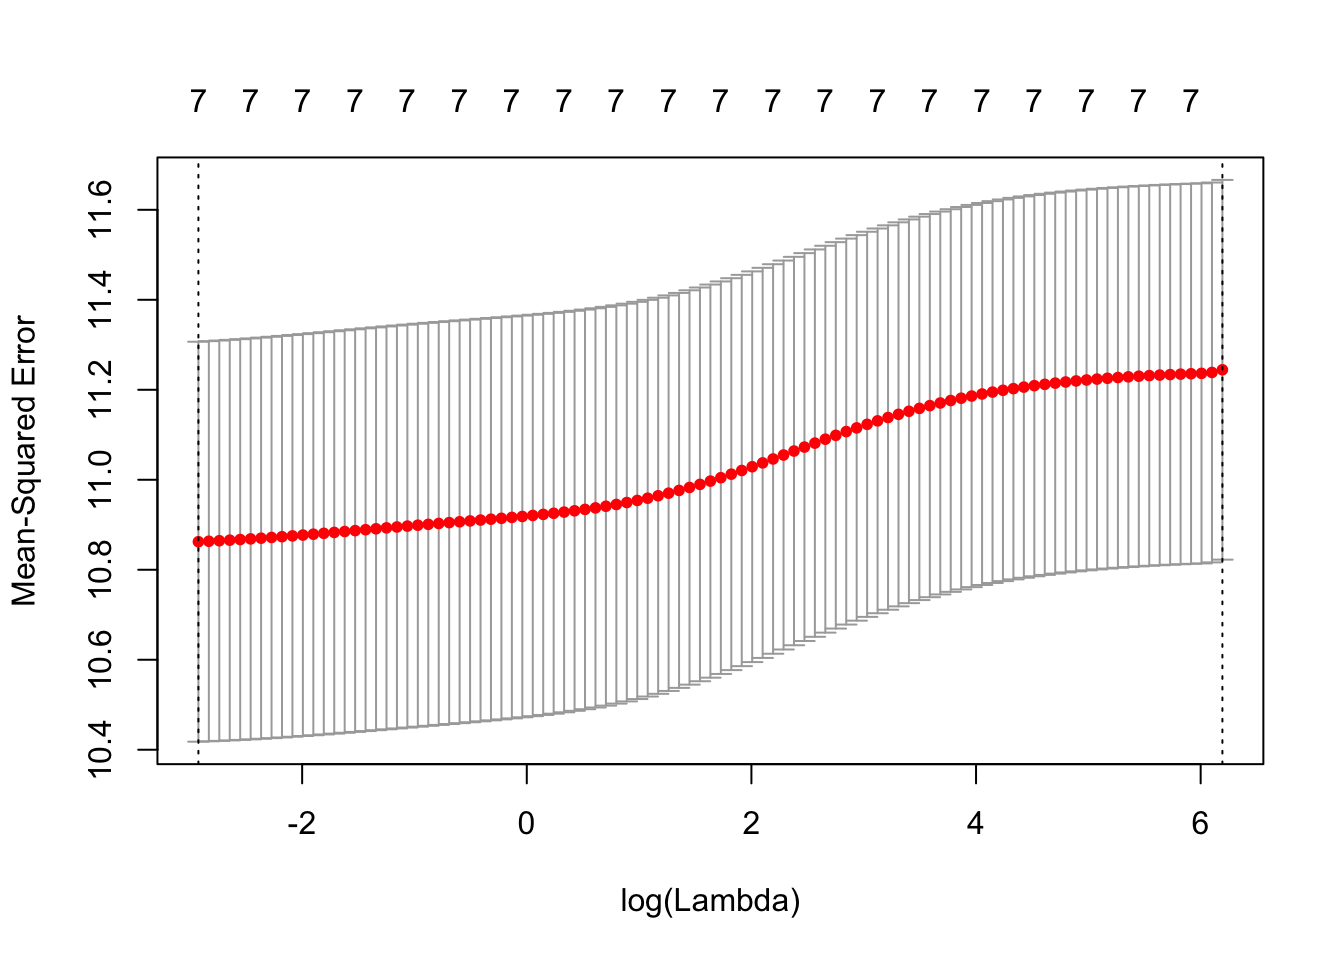
\includegraphics{_main_files/figure-latex/unnamed-chunk-107-1}

\begin{Shaded}
\begin{Highlighting}[]
\KeywordTok{plot}\NormalTok{(fit_lasso)}
\end{Highlighting}
\end{Shaded}

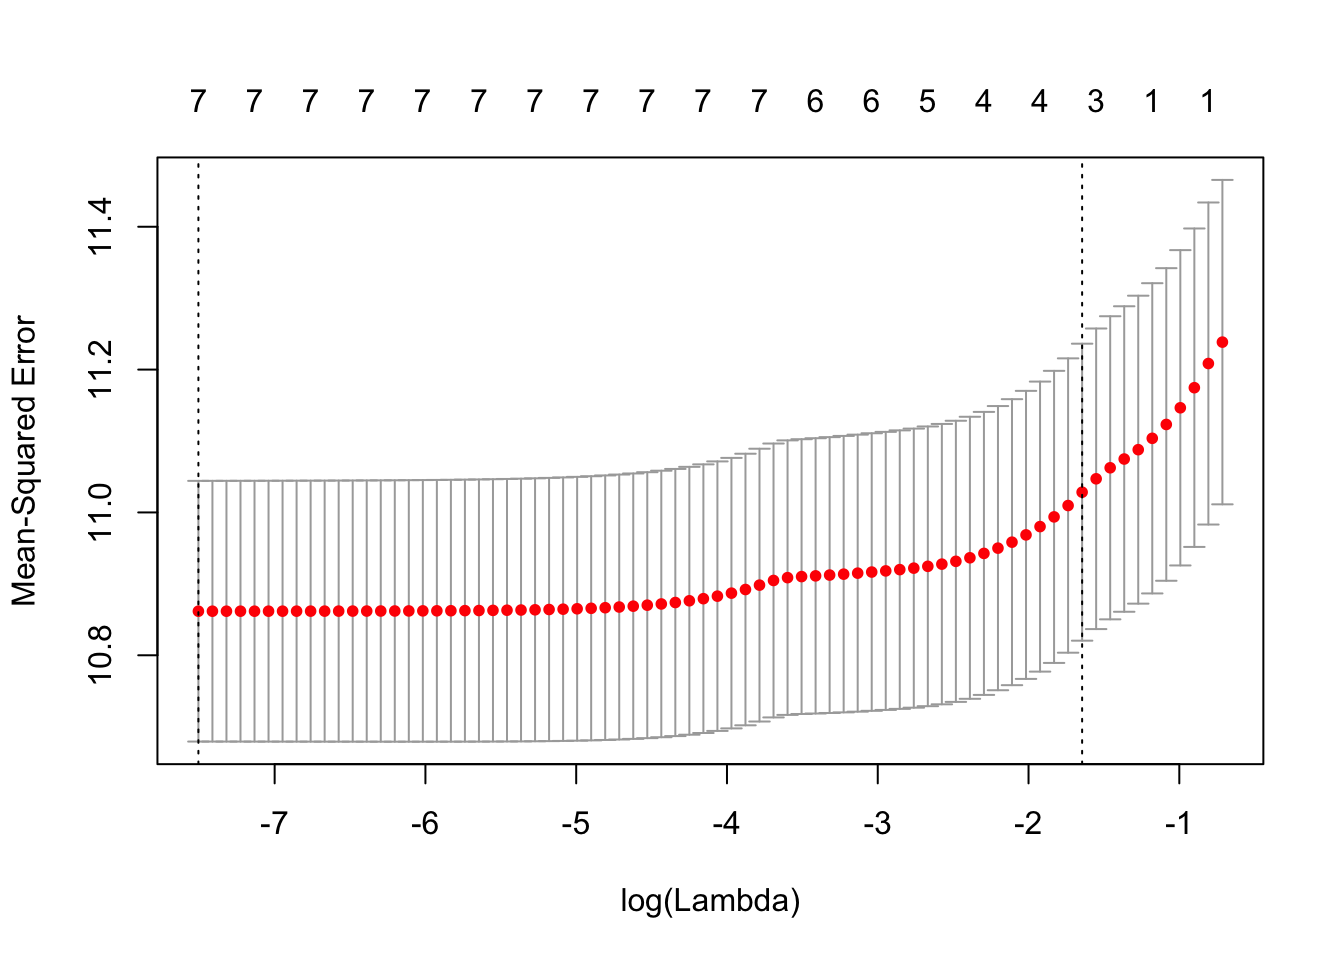
\includegraphics{_main_files/figure-latex/unnamed-chunk-107-2}

\begin{Shaded}
\begin{Highlighting}[]
\KeywordTok{plot}\NormalTok{(fit_enet)}
\end{Highlighting}
\end{Shaded}

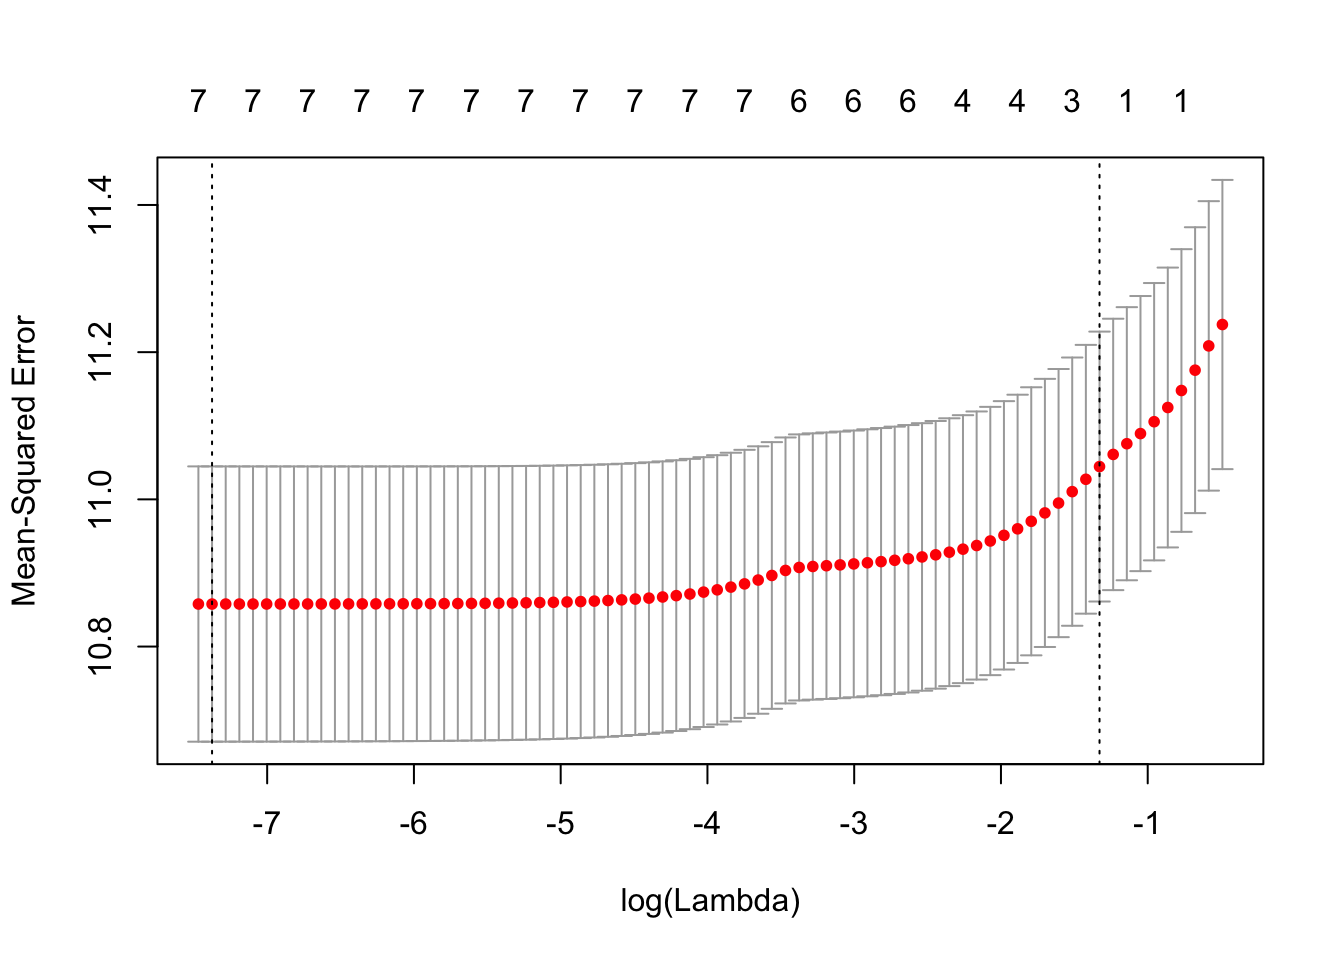
\includegraphics{_main_files/figure-latex/unnamed-chunk-107-3}

We can get the coefficients at a reasonable \texttt{lambda}.
Specifically, we use the ``1-SE rule'' (near the right hand side
vertical dashed lines in the above plots) by
\texttt{s\ =\ "lambda.1se"}. You can directly tell it what
\texttt{lambda} value you'd like but this is a simple rule of thumb.

\begin{Shaded}
\begin{Highlighting}[]
\KeywordTok{coef}\NormalTok{(fit_ridge, }\DataTypeTok{s =} \StringTok{"lambda.1se"}\NormalTok{)}
\end{Highlighting}
\end{Shaded}

\begin{verbatim}
## 8 x 1 sparse Matrix of class "dgCMatrix"
##                     1
## (Intercept)  5.827993
## riagendr     0.024703
## ridageyr    -0.000299
## ridreth3     0.031777
## race         0.050890
## famsize     -0.022046
## dep          0.005774
## asthma       0.056677
\end{verbatim}

\begin{Shaded}
\begin{Highlighting}[]
\KeywordTok{coef}\NormalTok{(fit_lasso, }\DataTypeTok{s =} \StringTok{"lambda.1se"}\NormalTok{)}
\end{Highlighting}
\end{Shaded}

\begin{verbatim}
## 8 x 1 sparse Matrix of class "dgCMatrix"
##                 1
## (Intercept) 5.465
## riagendr    .    
## ridageyr    .    
## ridreth3    .    
## race        0.209
## famsize     .    
## dep         .    
## asthma      .
\end{verbatim}

\begin{Shaded}
\begin{Highlighting}[]
\KeywordTok{coef}\NormalTok{(fit_enet, }\DataTypeTok{s =} \StringTok{"lambda.1se"}\NormalTok{)}
\end{Highlighting}
\end{Shaded}

\begin{verbatim}
## 8 x 1 sparse Matrix of class "dgCMatrix"
##                 1
## (Intercept) 5.478
## riagendr    .    
## ridageyr    .    
## ridreth3    .    
## race        0.205
## famsize     .    
## dep         .    
## asthma      .
\end{verbatim}

Although we briefly introduce these regression methods, they are indeed
very important. We highly recommend learning more about them.

\subsection*{Random Forests}\label{random-forests}
\addcontentsline{toc}{subsection}{Random Forests}

Random forests is another machine learning method that can do fantastic
prediction. It is built in a very different way than the methods we have
discussed up to this point. It is not built on a linear modeling scheme;
rather, it is built on classification and regression trees (CART).
Again, ``Introduction to Statistical Learning'' is a great resource to
learn more.

Conveniently, we can use the \texttt{randomForest} package. We specify
the model by the formula \texttt{sed\_hr\ \textasciitilde{}\ .} which
means we want \texttt{sed\_hr} to be the outcome and all the rest of the
variables to be predictors.

\begin{Shaded}
\begin{Highlighting}[]
\KeywordTok{library}\NormalTok{(randomForest)}

\NormalTok{fit_rf <-}\StringTok{ }\KeywordTok{randomForest}\NormalTok{(sed_hr }\OperatorTok{~}\StringTok{ }\NormalTok{., }\DataTypeTok{data =}\NormalTok{ df2)}
\NormalTok{fit_rf}
\end{Highlighting}
\end{Shaded}

\begin{verbatim}
## 
## Call:
##  randomForest(formula = sed_hr ~ ., data = df2) 
##                Type of random forest: regression
##                      Number of trees: 500
## No. of variables tried at each split: 2
## 
##           Mean of squared residuals: 10.8
##                     % Var explained: 3.87
\end{verbatim}

We can find out which variables were important in the model via:

\begin{Shaded}
\begin{Highlighting}[]
\KeywordTok{par}\NormalTok{(}\DataTypeTok{mfrow =} \KeywordTok{c}\NormalTok{(}\DecValTok{1}\NormalTok{, }\DecValTok{1}\NormalTok{))  ## back to one plot per page}
\KeywordTok{varImpPlot}\NormalTok{(fit_rf)}
\end{Highlighting}
\end{Shaded}

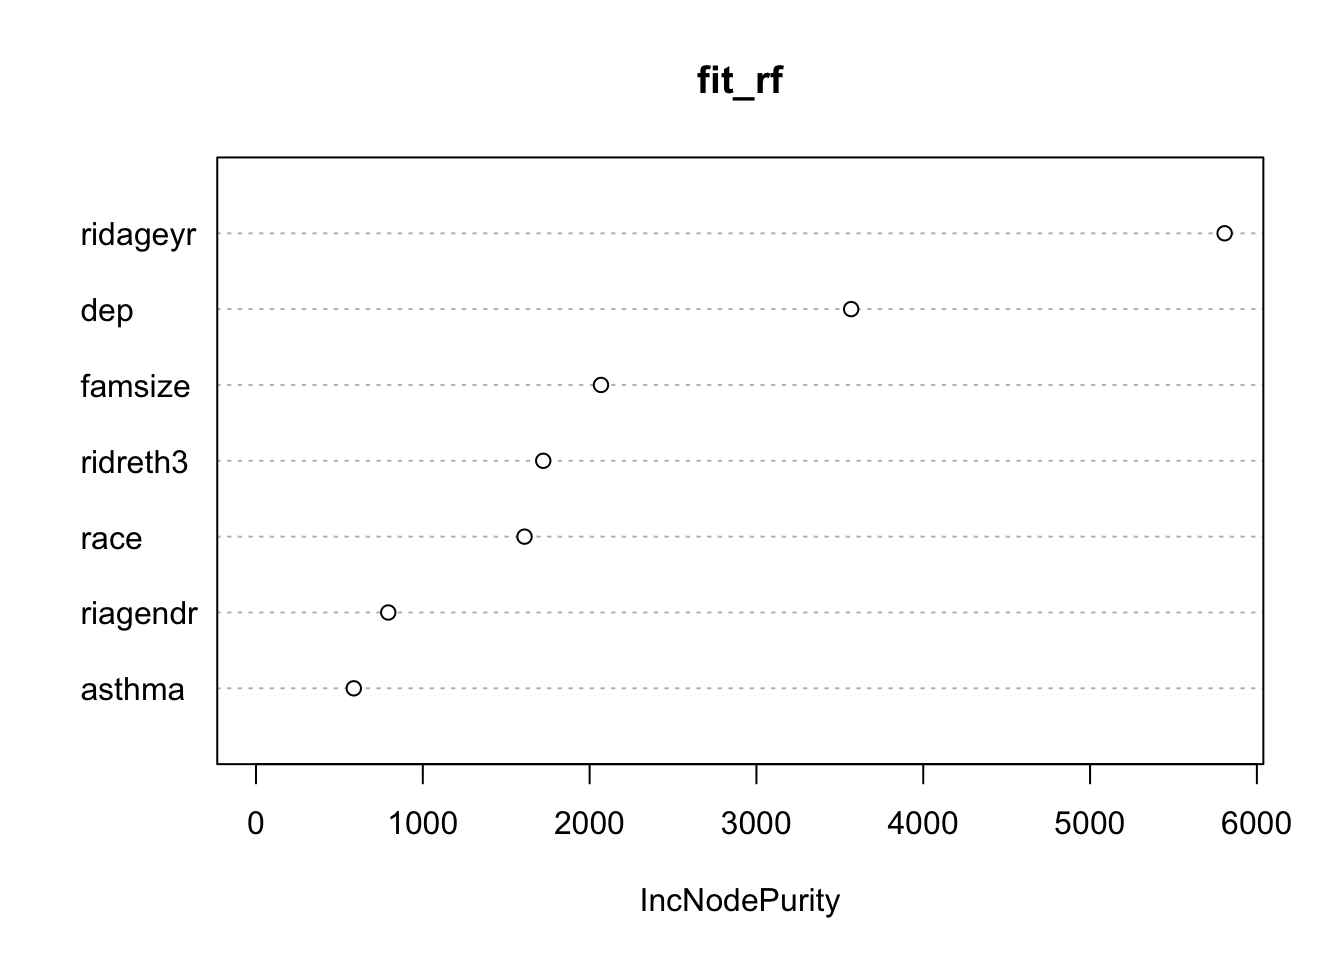
\includegraphics{_main_files/figure-latex/unnamed-chunk-110-1}

We can see that age (\texttt{ridageyr}) is the most important variable,
depression (\texttt{dep}) follows, with the family size
(\texttt{famsize}) the third most important in the random forests model.

\section*{Conclusions}\label{conclusions-3}
\addcontentsline{toc}{section}{Conclusions}

Although we only discussed these methods briefly, that does not mean
they are less important. On the contrary, they are essential upper level
statistical methods. This brief introduction hopefully helped you know
what \texttt{R} is capable of across a wide range of methods.

The next chapter begins our ``advanced'' topics, starting with
``Advanced Data Manipulation''.

\chapter*{Chapter 8: Advanced Data
Manipulation}\label{chapter-8-advanced-data-manipulation}
\addcontentsline{toc}{chapter}{Chapter 8: Advanced Data Manipulation}

\begin{quote}
``Every new thing creates two new questions and two new opportunities.''

--- Jeff Bezos
\end{quote}

There's so much more we can do with data in \texttt{R} than what we've
presented. Two main topics we need to clarify here are:

\begin{enumerate}
\def\labelenumi{\arabic{enumi}.}
\tightlist
\item
  How do you reshape your data from wide to long form or vice versa?
\item
  How do can we simplify tasks that we need done many times?
\end{enumerate}

We will introduce both ideas to you in this chapter. To discuss the
first, we will introduce two functions to help you reshape your data:
\texttt{gather()} and \texttt{spread()}. For the second, we need to talk
about loops. Looping, for our purposes, refers to the ability to repeat
something across many variables or data sets. There's many ways of doing
this but some are better than others. For looping, we'll talk about:

\begin{enumerate}
\def\labelenumi{\arabic{enumi}.}
\tightlist
\item
  vectorized functions,
\item
  \texttt{for} loops, and
\item
  the \texttt{apply} family of functions.
\end{enumerate}

\section*{Reshaping Your Data}\label{reshaping-your-data}
\addcontentsline{toc}{section}{Reshaping Your Data}

We introduced you to wide form and long form of your data in Chapter 2.
In reality, data can take on nearly infinite forms but for most data in
health, behavior, and social science, these two forms are sufficient to
know. But the question is, how to change the form of your data?

In the \texttt{tidyverse} functions known as \texttt{gather} and
\texttt{spread} can help with this in a simple way. To show you, we will
use the fake data we started with in Chapter 2.

\begin{verbatim}
##    ID Var_Time1 Var_Time2
## 1   1   -1.8052    0.0968
## 2   2   -1.1567    0.6295
## 3   3   -1.9489    0.0814
## 4   4   -0.4470    0.3412
## 5   5    1.1574    0.9422
## 6   6   -0.9718    0.5341
## 7   7   -0.4579    0.2252
## 8   8   -0.0479    0.5885
## 9   9   -0.1037    0.3071
## 10 10   -0.5246    0.7607
\end{verbatim}

Notice that this data frame is in wide format (each ID is one row and
there are multiple times or measurements per person). To change this to
wide format, we'll use \texttt{gather()}. The first argument is the
data.frame, followed by two variable names (names that we go into the
new long form), and then the numbers of the columns that are the
measures (in this case, \texttt{Var\_Time1} and \texttt{Var\_Time2}).

\begin{Shaded}
\begin{Highlighting}[]
\KeywordTok{library}\NormalTok{(tidyverse)}
\NormalTok{long_form <-}\StringTok{ }\KeywordTok{gather}\NormalTok{(d1, }\StringTok{"measures"}\NormalTok{, }\StringTok{"values"}\NormalTok{, }
    \DecValTok{2}\OperatorTok{:}\DecValTok{3}\NormalTok{)}
\NormalTok{long_form}
\end{Highlighting}
\end{Shaded}

\begin{verbatim}
##    ID  measures  values
## 1   1 Var_Time1 -1.8052
## 2   2 Var_Time1 -1.1567
## 3   3 Var_Time1 -1.9489
## 4   4 Var_Time1 -0.4470
## 5   5 Var_Time1  1.1574
## 6   6 Var_Time1 -0.9718
## 7   7 Var_Time1 -0.4579
## 8   8 Var_Time1 -0.0479
## 9   9 Var_Time1 -0.1037
## 10 10 Var_Time1 -0.5246
## 11  1 Var_Time2  0.0968
## 12  2 Var_Time2  0.6295
## 13  3 Var_Time2  0.0814
## 14  4 Var_Time2  0.3412
## 15  5 Var_Time2  0.9422
## 16  6 Var_Time2  0.5341
## 17  7 Var_Time2  0.2252
## 18  8 Var_Time2  0.5885
## 19  9 Var_Time2  0.3071
## 20 10 Var_Time2  0.7607
\end{verbatim}

As you can see, it took the variable names and put that in our first
variable that we called ``measures''. The actual values of the variables
are now in the variable we called ``values''. Finally, notice that each
ID now has two rows (one for each measure).

To go in the opposite direction (long to wide) we can use the
\texttt{spread()} function. All we do is provide the long formed data
frame, the measured variable (\texttt{measures}) and the variable with
the values (\texttt{values}).

\begin{Shaded}
\begin{Highlighting}[]
\NormalTok{wide_form <-}\StringTok{ }\KeywordTok{spread}\NormalTok{(long_form, measures, values)}
\NormalTok{wide_form}
\end{Highlighting}
\end{Shaded}

\begin{verbatim}
##    ID Var_Time1 Var_Time2
## 1   1   -1.8052    0.0968
## 2   2   -1.1567    0.6295
## 3   3   -1.9489    0.0814
## 4   4   -0.4470    0.3412
## 5   5    1.1574    0.9422
## 6   6   -0.9718    0.5341
## 7   7   -0.4579    0.2252
## 8   8   -0.0479    0.5885
## 9   9   -0.1037    0.3071
## 10 10   -0.5246    0.7607
\end{verbatim}

And we are back to the wide form.

These steps can be followed for situations where there are many measures
per person, many people per cluster, etc. In most cases, this is the way
multilevel data analysis occurs (as we discussed in Chapter 6) and is a
nice way to get our data ready for plotting.

\subsection*{\texorpdfstring{The \texttt{reshape()}
function}{The reshape() function}}\label{the-reshape-function}
\addcontentsline{toc}{subsection}{The \texttt{reshape()} function}

It is also possible to do multiple measures at once when moving from
wide to long or long to wide. The following figure shows the basics of
the \texttt{reshape()} function that was made for an introductory R
class (which can also be found
\href{https://tysonstanley.github.io/assets/images/DataCleaning_Handout.pdf}{here}).

\begin{figure}
\centering
\includegraphics{~/Desktop/DataCleaningHandout.png}
\caption{Reshape}
\end{figure}

Note a few important features:

\begin{enumerate}
\def\labelenumi{\arabic{enumi}.}
\tightlist
\item
  \texttt{reshape()} is used for moving from wide to long and long to
  wide. Here we just tell it the direction.
\item
  To indicate multiple columns, use a list of vectors (e.g.,
  \texttt{list(c("x1",\ "x2"),\ c("z1",\ "z2")))}).
\item
  \texttt{reshape()} can be used before or after subsetting, allowing
  for only the necessary variables to be included in the reshaping
  process.
\end{enumerate}

\section*{Repeating Actions (Looping)}\label{repeating-actions-looping}
\addcontentsline{toc}{section}{Repeating Actions (Looping)}

To fully go into looping, understanding how to write your own functions
is needed.

\subsection*{Your Own Functions}\label{your-own-functions}
\addcontentsline{toc}{subsection}{Your Own Functions}

Let's create a function that estimates the mean (although it is
completely unnecessary since there is already a perfectly good
\texttt{mean()} function).

\begin{Shaded}
\begin{Highlighting}[]
\NormalTok{mean2 <-}\StringTok{ }\ControlFlowTok{function}\NormalTok{(x) \{}
\NormalTok{    n <-}\StringTok{ }\KeywordTok{length}\NormalTok{(x)}
\NormalTok{    m <-}\StringTok{ }\NormalTok{(}\DecValTok{1}\OperatorTok{/}\NormalTok{n) }\OperatorTok{*}\StringTok{ }\KeywordTok{sum}\NormalTok{(x)}
    \KeywordTok{return}\NormalTok{(m)}
\NormalTok{\}}
\end{Highlighting}
\end{Shaded}

We create a function using the \texttt{function()} function.\footnote{That
  seemed like excessive use of the word function\ldots{} It is important
  though. So, get used to it!} Within the \texttt{function()} we put an
\texttt{x}. This is the argument that the function will ask for. Here,
it is a numeric vector that we want to take the mean of. We then provide
the meat of the function between the \texttt{\{\}}. Here, we did a
simple mean calculation using the \texttt{length(x)} which gives us the
number of observations, and \texttt{sum()} which sums the numbers in
\texttt{x}.

Let's give it a try:

\begin{Shaded}
\begin{Highlighting}[]
\NormalTok{v1 <-}\StringTok{ }\KeywordTok{c}\NormalTok{(}\DecValTok{1}\NormalTok{, }\DecValTok{3}\NormalTok{, }\DecValTok{2}\NormalTok{, }\DecValTok{4}\NormalTok{, }\DecValTok{2}\NormalTok{, }\DecValTok{1}\NormalTok{, }\DecValTok{2}\NormalTok{, }\DecValTok{1}\NormalTok{, }\DecValTok{1}\NormalTok{, }\DecValTok{1}\NormalTok{)  ## vector to try}
\KeywordTok{mean2}\NormalTok{(v1)  ## our function}
\end{Highlighting}
\end{Shaded}

\begin{verbatim}
## [1] 1.8
\end{verbatim}

\begin{Shaded}
\begin{Highlighting}[]
\KeywordTok{mean}\NormalTok{(v1)  ## the base R function}
\end{Highlighting}
\end{Shaded}

\begin{verbatim}
## [1] 1.8
\end{verbatim}

Looks good! These functions that you create can do whatever you need
them to (within the bounds that \texttt{R} can do). I recommend by
starting outside of a function that then put it into a function. For
example, we would start with:

\begin{Shaded}
\begin{Highlighting}[]
\NormalTok{n <-}\StringTok{ }\KeywordTok{length}\NormalTok{(v1)}
\NormalTok{m <-}\StringTok{ }\NormalTok{(}\DecValTok{1}\OperatorTok{/}\NormalTok{n) }\OperatorTok{*}\StringTok{ }\KeywordTok{sum}\NormalTok{(v1)}
\NormalTok{m}
\end{Highlighting}
\end{Shaded}

\begin{verbatim}
## [1] 1.8
\end{verbatim}

and once things look good, we would put it into a function like we had
before with \texttt{mean2}. It is an easy way to develop a good function
and test it while developing it.

By creating your own function, you can simplify your workflow and can
use them in loops, the \texttt{apply} functions and the \texttt{purrr}
package.

For practice, we will write one more function. Let's make a function
that takes a vector and gives us the N, the mean, and the standard
deviation.

\begin{Shaded}
\begin{Highlighting}[]
\NormalTok{important_statistics <-}\StringTok{ }\ControlFlowTok{function}\NormalTok{(x, }\DataTypeTok{na.rm =} \OtherTok{FALSE}\NormalTok{) \{}
\NormalTok{    N <-}\StringTok{ }\KeywordTok{length}\NormalTok{(x)}
\NormalTok{    M <-}\StringTok{ }\KeywordTok{mean}\NormalTok{(x, }\DataTypeTok{na.rm =}\NormalTok{ na.rm)}
\NormalTok{    SD <-}\StringTok{ }\KeywordTok{sd}\NormalTok{(x, }\DataTypeTok{na.rm =}\NormalTok{ na.rm)}
    
\NormalTok{    final <-}\StringTok{ }\KeywordTok{c}\NormalTok{(N, M, SD)}
    \KeywordTok{return}\NormalTok{(final)}
\NormalTok{\}}
\end{Highlighting}
\end{Shaded}

One of the first things you should note is that we included a second
argument in the function seen as \texttt{na.rm=FALSE} (you can have as
many arguments as you want within reason). This argument has a default
that we provide as \texttt{FALSE} as it is in most functions that use
the \texttt{na.rm} argument. We take what is provided in the
\texttt{na.rm} and give that to both the \texttt{mean()} and
\texttt{sd()} functions. Finally, you should notice that we took several
pieces of information and combined them into the \texttt{final} object
and returned that.

Let's try it out with the vector we created earlier.

\begin{Shaded}
\begin{Highlighting}[]
\KeywordTok{important_statistics}\NormalTok{(v1)}
\end{Highlighting}
\end{Shaded}

\begin{verbatim}
## [1] 10.00  1.80  1.03
\end{verbatim}

Looks good but we may want to change a few aesthetics. In the following
code, we adjust it so we have each one labeled.

\begin{Shaded}
\begin{Highlighting}[]
\NormalTok{important_statistics2 <-}\StringTok{ }\ControlFlowTok{function}\NormalTok{(x, }\DataTypeTok{na.rm =} \OtherTok{FALSE}\NormalTok{) \{}
\NormalTok{    N <-}\StringTok{ }\KeywordTok{length}\NormalTok{(x)}
\NormalTok{    M <-}\StringTok{ }\KeywordTok{mean}\NormalTok{(x, }\DataTypeTok{na.rm =}\NormalTok{ na.rm)}
\NormalTok{    SD <-}\StringTok{ }\KeywordTok{sd}\NormalTok{(x, }\DataTypeTok{na.rm =}\NormalTok{ na.rm)}
    
\NormalTok{    final <-}\StringTok{ }\KeywordTok{data.frame}\NormalTok{(N, }\DataTypeTok{Mean =}\NormalTok{ M, }\DataTypeTok{SD =}\NormalTok{ SD)}
    \KeywordTok{return}\NormalTok{(final)}
\NormalTok{\}}
\KeywordTok{important_statistics2}\NormalTok{(v1)}
\end{Highlighting}
\end{Shaded}

\begin{verbatim}
##    N Mean   SD
## 1 10  1.8 1.03
\end{verbatim}

We will come back to this function and use it in some loops and see what
else we can do with it.

\subsection*{Vectorized}\label{vectorized}
\addcontentsline{toc}{subsection}{Vectorized}

By construction, \texttt{R} is the fastest when we use the vectorized
form of doing things. For example, when we want to add two variables
together, we can use the \texttt{+} operator. Like most functions in
\texttt{R}, it is vectorized and so it is fast. Below we create a new
vector using the \texttt{rnorm()} function that produces normally
distributed random variables. First argument in the function is the
length of the vector, followed by the mean and SD.

\begin{Shaded}
\begin{Highlighting}[]
\NormalTok{v2 <-}\StringTok{ }\KeywordTok{rnorm}\NormalTok{(}\DecValTok{10}\NormalTok{, }\DataTypeTok{mean =} \DecValTok{5}\NormalTok{, }\DataTypeTok{sd =} \DecValTok{2}\NormalTok{)}
\NormalTok{add1 <-}\StringTok{ }\NormalTok{v1 }\OperatorTok{+}\StringTok{ }\NormalTok{v2}
\KeywordTok{round}\NormalTok{(add1, }\DecValTok{3}\NormalTok{)}
\end{Highlighting}
\end{Shaded}

\begin{verbatim}
##  [1] 2.28 5.73 4.22 6.11 6.92 6.57 5.51 7.36
##  [9] 7.28 6.71
\end{verbatim}

We will compare the speed of this to other ways of adding two variables
together and see it is the simplest and quickest.

\subsection*{For Loops}\label{for-loops}
\addcontentsline{toc}{subsection}{For Loops}

For loops have a bad reputation in the \texttt{R} world. This is
because, in general, they are slow. It is among the slowest of ways to
iterate (i.e., repeat) functions. We start here to show you, in essence,
what the \texttt{apply} family of functions are doing, often, in a
faster way.

At times, it is easiest to develop a for loop and then take it and use
it within the \texttt{apply} or \texttt{purrr} functions. It can help
you think through the pieces that need to be done in order to get your
desired result.

For demonstration, we are using the \texttt{for} loop to add two
variables together. The code between the \texttt{()}'s tells \texttt{R}
information about how many loops it should do. Here, we are looping
through \texttt{1:10} since there are ten observations in each vector.
We could also specify this as \texttt{1:length(v1)}. When using
\texttt{for} loops, we need to keep in mind that we need to initialize a
variable in order to use it within the loop. That's precisely what we do
with the \texttt{add2}, making it a numberic vector with 10
observations.

\begin{Shaded}
\begin{Highlighting}[]
\NormalTok{add2 <-}\StringTok{ }\KeywordTok{vector}\NormalTok{(}\StringTok{"numeric"}\NormalTok{, }\DecValTok{10}\NormalTok{)  ## Initialize}
\ControlFlowTok{for}\NormalTok{ (i }\ControlFlowTok{in} \DecValTok{1}\OperatorTok{:}\DecValTok{10}\NormalTok{) \{}
\NormalTok{    add2[i] <-}\StringTok{ }\NormalTok{v1[i] }\OperatorTok{+}\StringTok{ }\NormalTok{v2[i]}
\NormalTok{\}}
\KeywordTok{round}\NormalTok{(add2, }\DecValTok{3}\NormalTok{)}
\end{Highlighting}
\end{Shaded}

\begin{verbatim}
##  [1] 2.28 5.73 4.22 6.11 6.92 6.57 5.51 7.36
##  [9] 7.28 6.71
\end{verbatim}

Same results! But, we'll see later that the speed is much than the
vectorized function.

\subsection*{\texorpdfstring{The \texttt{apply}
family}{The apply family}}\label{the-apply-family}
\addcontentsline{toc}{subsection}{The \texttt{apply} family}

The \texttt{apply} family of functions that we'll introduce are:

\begin{enumerate}
\def\labelenumi{\arabic{enumi}.}
\tightlist
\item
  \texttt{apply()}
\item
  \texttt{lapply()}
\item
  \texttt{sapply()}
\item
  \texttt{tapply()}
\end{enumerate}

Each essentially do a loop over the data you provide using a function
(either one you created or another). The different versions are
extremely similar with some minor differences. For \texttt{apply()} you
tell it if you want to iterative over the columns or rows;
\texttt{lapply()} assumes you want to iterate over the columns and
outputs a list (hence the \texttt{l}); \texttt{sapply()} is similar to
\texttt{lapply()} but outputs vectors and data frames. \texttt{tapply()}
has the most differences because it can iterative over columns by a
grouping variable. We'll show \texttt{apply()}, \texttt{lapply()} and
\texttt{tapply()} below.

For example, we can add two variables together here. We provide it the
\texttt{data.frame} that has the variables we want to add together.

\begin{Shaded}
\begin{Highlighting}[]
\NormalTok{df <-}\StringTok{ }\KeywordTok{data.frame}\NormalTok{(v1, v2)}
\NormalTok{add3 <-}\StringTok{ }\KeywordTok{apply}\NormalTok{(df, }\DecValTok{1}\NormalTok{, sum)}
\KeywordTok{round}\NormalTok{(add3, }\DecValTok{3}\NormalTok{)}
\end{Highlighting}
\end{Shaded}

\begin{verbatim}
##  [1] 2.28 5.73 4.22 6.11 6.92 6.57 5.51 7.36
##  [9] 7.28 6.71
\end{verbatim}

The function \texttt{apply()} has three main arguments: a) the
\texttt{data.frame} or list of data, b) 1 meaning to apply the function
for each row or 2 to the columns, and c) the function to use.

We can also use one of our own functions such as
\texttt{important\_statistics2()} within the \texttt{apply} family.

\begin{Shaded}
\begin{Highlighting}[]
\KeywordTok{lapply}\NormalTok{(df, important_statistics2)}
\end{Highlighting}
\end{Shaded}

\begin{verbatim}
## $v1
##    N Mean   SD
## 1 10  1.8 1.03
## 
## $v2
##    N Mean   SD
## 1 10 4.07 1.91
\end{verbatim}

This gives us a list of two elements, one for each variable, with the
statistics that our function provides. With a little adjustment, we can
make this into a \texttt{data.frame} using the \texttt{do.call()}
function with \texttt{"rbind"}.

\begin{Shaded}
\begin{Highlighting}[]
\KeywordTok{do.call}\NormalTok{(}\StringTok{"rbind"}\NormalTok{, }\KeywordTok{lapply}\NormalTok{(df, important_statistics2))}
\end{Highlighting}
\end{Shaded}

\begin{verbatim}
##     N Mean   SD
## v1 10 1.80 1.03
## v2 10 4.07 1.91
\end{verbatim}

\texttt{tapply()} allows us to get information by a grouping factor. We
are going to add a factor variable to the data frame we are using
\texttt{df} and then get the mean of the variables by group.

\begin{Shaded}
\begin{Highlighting}[]
\NormalTok{group1 <-}\StringTok{ }\KeywordTok{factor}\NormalTok{(}\KeywordTok{sample}\NormalTok{(}\KeywordTok{c}\NormalTok{(}\DecValTok{0}\NormalTok{, }\DecValTok{1}\NormalTok{), }\DecValTok{10}\NormalTok{, }\DataTypeTok{replace =} \OtherTok{TRUE}\NormalTok{))}
\KeywordTok{tapply}\NormalTok{(df}\OperatorTok{$}\NormalTok{v1, group1, mean)}
\end{Highlighting}
\end{Shaded}

\begin{verbatim}
##   0   1 
## 1.6 2.0
\end{verbatim}

We now have the means by each group. This, however, is probably replaced
by the 3 step summary that we learned earlier in \texttt{dplyr} using
\texttt{group\_by()} and \texttt{summarize()}.

These functions are useful in many situations, especially where there
are no vectorized functions. You can always get an idea of whether to
use a \texttt{for} loop or an \texttt{apply} function by giving it a try
on a small subset of data to see if one is better and/or faster.

\subsubsection*{Speed Comparison}\label{speed-comparison}
\addcontentsline{toc}{subsubsection}{Speed Comparison}

We can test to see how fast functions are with the
\texttt{microbenchmark} package. Since it wants functions, we will
create a function that uses the \texttt{for} looop.

\begin{Shaded}
\begin{Highlighting}[]
\NormalTok{forloop <-}\StringTok{ }\ControlFlowTok{function}\NormalTok{(var1, var2) \{}
\NormalTok{    add2 <-}\StringTok{ }\KeywordTok{vector}\NormalTok{(}\StringTok{"numeric"}\NormalTok{, }\KeywordTok{length}\NormalTok{(var1))}
    \ControlFlowTok{for}\NormalTok{ (i }\ControlFlowTok{in} \DecValTok{1}\OperatorTok{:}\DecValTok{10}\NormalTok{) \{}
\NormalTok{        add2[i] <-}\StringTok{ }\NormalTok{var1[i] }\OperatorTok{+}\StringTok{ }\NormalTok{var2[i]}
\NormalTok{    \}}
    \KeywordTok{return}\NormalTok{(add2)}
\NormalTok{\}}
\end{Highlighting}
\end{Shaded}

Below, we can see that the vectorized version is nearly 50 times faster
than the \texttt{for} loop and 300 times faster than the \texttt{apply}.
Although the \texttt{for} loop was faster here, sometimes it can be
slower than the \texttt{apply} functions--it just depends on the
situation. But, the vectorized functions will almost always be
\emph{much} faster than anything else. It's important to note that the
\texttt{+} is also a function that can be used as we do below,
highlighting the fact that anything that does something to an object in
\texttt{R} is a function.

\begin{Shaded}
\begin{Highlighting}[]
\KeywordTok{library}\NormalTok{(microbenchmark)}
\KeywordTok{microbenchmark}\NormalTok{(}\KeywordTok{forloop}\NormalTok{(v1, v2), }\KeywordTok{apply}\NormalTok{(df, }\DecValTok{1}\NormalTok{, sum), }
\NormalTok{    v1 }\OperatorTok{+}\StringTok{ }\NormalTok{v2)}
\end{Highlighting}
\end{Shaded}

\begin{verbatim}
## Unit: nanoseconds
##               expr   min    lq  mean median
##    forloop(v1, v2)  9618 11006 17860  11882
##  apply(df, 1, sum) 76429 79856 96719  83450
##            v1 + v2   173   238   439    400
##      uq    max neval cld
##   13632 115079   100  b 
##  101504 322722   100   c
##     504   1850   100 a
\end{verbatim}

Of course, as it says the units are in nanoseconds. Whether a function
takes 200 or 200,000 nanoseconds probably won't change your life.
However, if the function is being used repeatedly or on on large data
sets, this can make a difference.

\subsection*{\texorpdfstring{Using ``Anonymous Functions'' in
Apply}{Using Anonymous Functions in Apply}}\label{using-anonymous-functions-in-apply}
\addcontentsline{toc}{subsection}{Using ``Anonymous Functions'' in
Apply}

Last thing to know here is that you don't need to create a named
function everytime you want to use \texttt{apply}. We can use what is
called ``Anonymous'' functions. Below, we use one to get at the N and
mean of the data.

\begin{Shaded}
\begin{Highlighting}[]
\KeywordTok{lapply}\NormalTok{(df, }\ControlFlowTok{function}\NormalTok{(x) }\KeywordTok{rbind}\NormalTok{(}\KeywordTok{length}\NormalTok{(x), }\KeywordTok{mean}\NormalTok{(x, }
    \DataTypeTok{na.rm =} \OtherTok{TRUE}\NormalTok{)))}
\end{Highlighting}
\end{Shaded}

\begin{verbatim}
## $v1
##      [,1]
## [1,] 10.0
## [2,]  1.8
## 
## $v2
##       [,1]
## [1,] 10.00
## [2,]  4.07
\end{verbatim}

So we don't name the function but we design it like we would a named
function, just minus the \texttt{return()}. We take \texttt{x} (which is
a column of \texttt{df}) and do \texttt{length()} and \texttt{mean()}
and bind them by rows. The first argument in the anonymous function will
be the column or variable of the data you provide.

Here's another example:

\begin{Shaded}
\begin{Highlighting}[]
\KeywordTok{lapply}\NormalTok{(df, }\ControlFlowTok{function}\NormalTok{(y) y }\OperatorTok{*}\StringTok{ }\DecValTok{2}\OperatorTok{/}\KeywordTok{sd}\NormalTok{(y))}
\end{Highlighting}
\end{Shaded}

\begin{verbatim}
## $v1
##  [1] 1.94 5.81 3.87 7.75 3.87 1.94 3.87 1.94
##  [9] 1.94 1.94
## 
## $v2
##  [1] 1.33 2.85 2.32 2.21 5.14 5.82 3.67 6.65
##  [9] 6.56 5.97
\end{verbatim}

We take \texttt{y} (again, the column of \texttt{df}), times it by two
and divide by the standard deviation of \texttt{y}. Note that this is
gibberish and is not some special formula, but again, we can see how
flexible it is.

The last two examples also show something important regarding the
output:

\begin{enumerate}
\def\labelenumi{\arabic{enumi}.}
\tightlist
\item
  The output will be at the level of the anonymous function. The first
  had two numbers per variable because the function produced two summary
  statistics for each variable. The second we multiplied \texttt{y} by 2
  (so it is still at the individual observation level) and then divide
  by the SD. This keeps it at the observation level so we get ten values
  for every variable.
\item
  We can name the argument anything we want (as long as it is one word).
  We used \texttt{x} in the first and \texttt{y} in the second but as
  long as it is the same within the function, it doesn't matter what you
  use.
\end{enumerate}

\section*{Conclusions}\label{conclusions-4}
\addcontentsline{toc}{section}{Conclusions}

These are useful tools to use in your own data manipulation beyond that
what we discussed with \texttt{dplyr}. It takes time to get used to
making your own functions so be patient with yourself as you learn how
to get \texttt{R} to do exactly what you want in a condensed, replicable
format.

With these new tricks up your sleeve, we can move on to more advanced
plotting using \texttt{ggplot2}.

\chapter*{Chapter 9: Advanced
Plotting}\label{chapter-9-advanced-plotting}
\addcontentsline{toc}{chapter}{Chapter 9: Advanced Plotting}

\begin{quote}
``The commonality between science and art is in trying to see profoundly
- to develop strategies of seeing and showing.''

--- Edward Tufte
\end{quote}

Once again, we will turn to our friend \texttt{ggplot2} to plot; but
now, we are going to take it to another level. We will use many of the
options that this powerful package provides and discuss briefly some
important aspects of a good plot.

We will go through several aspects of the code that makes plotting in
\texttt{R} flexible and beautiful.

\begin{enumerate}
\def\labelenumi{\arabic{enumi}.}
\tightlist
\item
  Types of plots
\item
  Color schemes
\item
  Themes
\item
  Labels and titles
\item
  Facetting
\end{enumerate}

To highlight these features we'll be using our NHANES data again;
specifically, sedentary behavior, depression, asthma, family size, and
race. As this is only an introduction, refer to
\url{http://docs.ggplot2.org/current/} for more information on
\texttt{ggplot2}.

To begin, it needs to be understood that the first line where we
actually use the \texttt{ggplot} function, will then apply to all
subsequent laters (e.g., \texttt{geom\_point()}). For example,

\begin{Shaded}
\begin{Highlighting}[]
\KeywordTok{ggplot}\NormalTok{(df, }\KeywordTok{aes}\NormalTok{(}\DataTypeTok{x =}\NormalTok{ dep, }\DataTypeTok{y =}\NormalTok{ sed, }\DataTypeTok{group =}\NormalTok{ asthma))}
\end{Highlighting}
\end{Shaded}

means for the rest of the layers, unless we over-ride it, each will use
\texttt{df} with \texttt{dep} as the x variable, \texttt{sed} as the y,
and a grouping on \texttt{asthma}. So when many layers are going to use
the same command put it in this so you don't have to write the same
argument many times. A common one here could be:

\begin{Shaded}
\begin{Highlighting}[]
\KeywordTok{ggplot}\NormalTok{(df, }\KeywordTok{aes}\NormalTok{(}\DataTypeTok{x =}\NormalTok{ dep, }\DataTypeTok{y =}\NormalTok{ sed, }\DataTypeTok{group =}\NormalTok{ asthma, }
    \DataTypeTok{color =}\NormalTok{ asthma))}
\end{Highlighting}
\end{Shaded}

since we often want to color by our grouping variable.

Before going forward, a nice feature of \texttt{ggplot2} allows us to
use an ``incomplete'' plot to add on to. For example, if we have a good
idea of the main structure of the plot but want to explore some changes,
we can do the following:

\begin{Shaded}
\begin{Highlighting}[]
\NormalTok{p1 <-}\StringTok{ }\KeywordTok{ggplot}\NormalTok{(df, }\KeywordTok{aes}\NormalTok{(}\DataTypeTok{x =}\NormalTok{ dep, }\DataTypeTok{y =}\NormalTok{ sed, }\DataTypeTok{group =}\NormalTok{ asthma)) }\OperatorTok{+}\StringTok{ }
\StringTok{    }\KeywordTok{geom_point}\NormalTok{()}
\NormalTok{p1}
\end{Highlighting}
\end{Shaded}

\begin{verbatim}
## Warning: Removed 18 rows containing missing values
## (geom_point).
\end{verbatim}

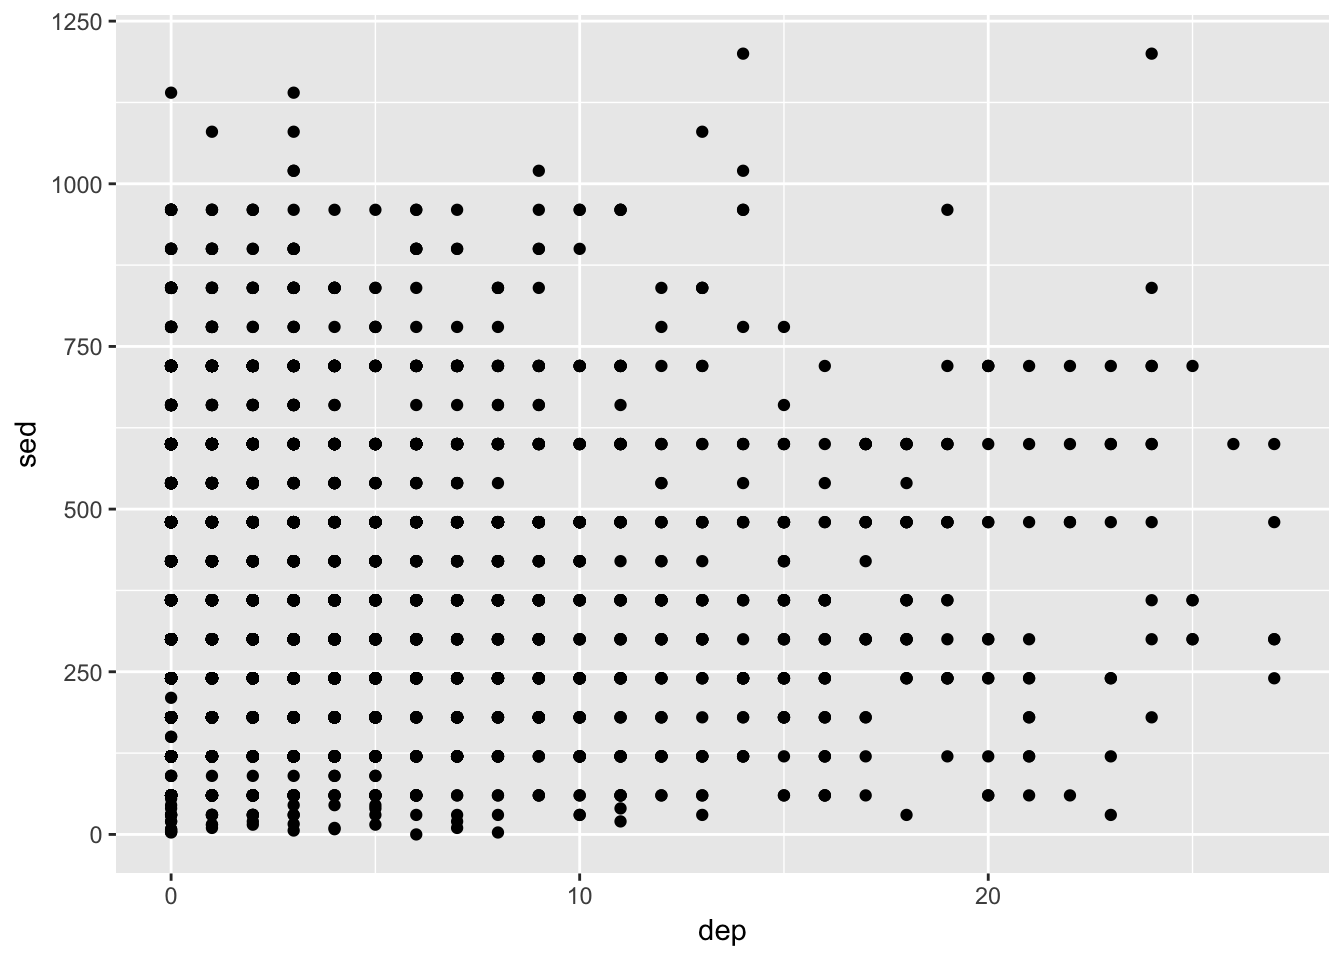
\includegraphics{_main_files/figure-latex/unnamed-chunk-133-1} So now
\texttt{p1} has the information for this basic, and honestly fairly
uninformative, plot. We'll use this feature to build on plots that we
like.

Some of our figures will also need summary data so we'll start that here
as well:

\begin{Shaded}
\begin{Highlighting}[]
\NormalTok{summed_data <-}\StringTok{ }\NormalTok{df }\OperatorTok\StringTok{ }\KeywordTok{group_by}\NormalTok{(asthma, dep2) }\OperatorTok\StringTok{ }
\StringTok{    }\KeywordTok{summarize}\NormalTok{(}\DataTypeTok{s_se =} \KeywordTok{sd}\NormalTok{(sed, }\DataTypeTok{na.rm =} \OtherTok{TRUE}\NormalTok{)}\OperatorTok{/}\KeywordTok{sqrt}\NormalTok{(}\KeywordTok{n}\NormalTok{()), }
        \DataTypeTok{sed =} \KeywordTok{mean}\NormalTok{(sed, }\DataTypeTok{na.rm =} \OtherTok{TRUE}\NormalTok{), }\DataTypeTok{N =} \KeywordTok{n}\NormalTok{())}
\end{Highlighting}
\end{Shaded}

As you hopefully recognize a bit, we are summarizing the time spent
being sedentary by both asthma and the dichotomous depression variables.
If it doesn't make sense at first, read it line by line to see what I
did. This will be useful for several types of plots.

\section*{Types of Plots}\label{types-of-plots}
\addcontentsline{toc}{section}{Types of Plots}

\subsection*{Scatterplots}\label{scatterplots}
\addcontentsline{toc}{subsection}{Scatterplots}

We'll start with a scatterplot--one of the most simple yet informative
plots.

\begin{Shaded}
\begin{Highlighting}[]
\KeywordTok{ggplot}\NormalTok{(df, }\KeywordTok{aes}\NormalTok{(}\DataTypeTok{x =}\NormalTok{ dep, }\DataTypeTok{y =}\NormalTok{ sed, }\DataTypeTok{group =}\NormalTok{ asthma)) }\OperatorTok{+}\StringTok{ }
\StringTok{    }\KeywordTok{geom_point}\NormalTok{(}\KeywordTok{aes}\NormalTok{(}\DataTypeTok{color =}\NormalTok{ asthma))}
\end{Highlighting}
\end{Shaded}

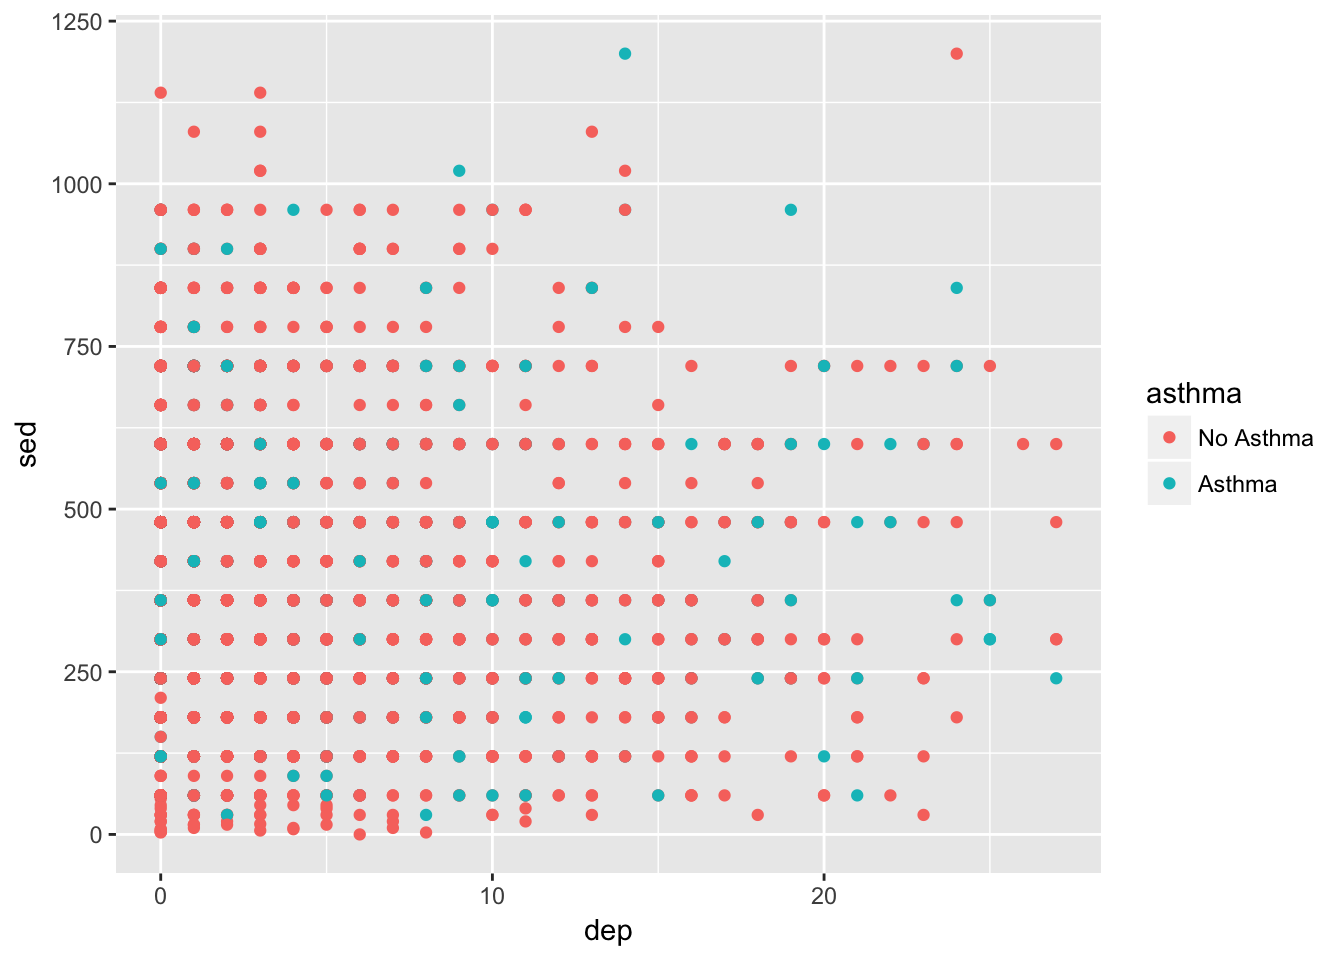
\includegraphics{_main_files/figure-latex/unnamed-chunk-135-1}

It's not amazing. There looks to be a lot of overlap of the points.
Also, it would be nice to know general trend lines for each group.
Below, \texttt{alpha} refers to how transparent the points are,
\texttt{method\ =\ "lm"} refers to how the line should be fit, and
\texttt{se=FALSE} tells it not to include error ribbons.

\begin{Shaded}
\begin{Highlighting}[]
\KeywordTok{ggplot}\NormalTok{(df, }\KeywordTok{aes}\NormalTok{(}\DataTypeTok{x =}\NormalTok{ dep, }\DataTypeTok{y =}\NormalTok{ sed, }\DataTypeTok{group =}\NormalTok{ asthma)) }\OperatorTok{+}\StringTok{ }
\StringTok{    }\KeywordTok{geom_jitter}\NormalTok{(}\KeywordTok{aes}\NormalTok{(}\DataTypeTok{color =}\NormalTok{ asthma), }\DataTypeTok{alpha =} \FloatTok{0.5}\NormalTok{) }\OperatorTok{+}\StringTok{ }
\StringTok{    }\KeywordTok{geom_smooth}\NormalTok{(}\KeywordTok{aes}\NormalTok{(}\DataTypeTok{color =}\NormalTok{ asthma), }\DataTypeTok{method =} \StringTok{"lm"}\NormalTok{, }
        \DataTypeTok{se =} \OtherTok{FALSE}\NormalTok{)}
\end{Highlighting}
\end{Shaded}

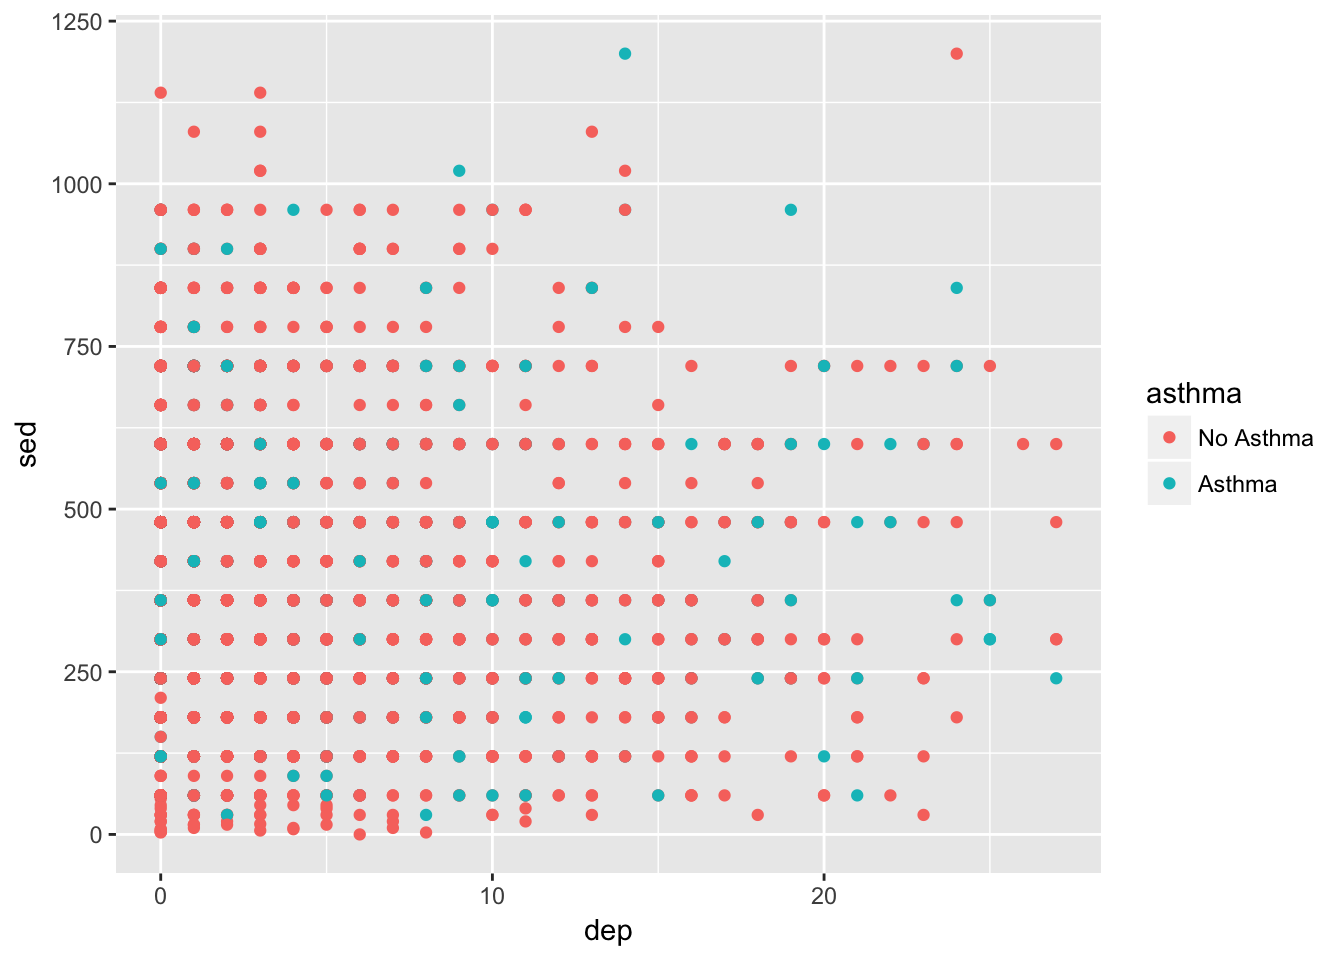
\includegraphics{_main_files/figure-latex/unnamed-chunk-136-1}

It's getting better but we could still use some more features. We'll
come back to this in the next sections.

\subsection*{Boxplots}\label{boxplots}
\addcontentsline{toc}{subsection}{Boxplots}

Box plots are great ways to assess the variability in your data. Below,
we create a boxplot but change \texttt{p1}'s x variable so that it is
the factor version of depression.

\begin{Shaded}
\begin{Highlighting}[]
\KeywordTok{ggplot}\NormalTok{(df, }\KeywordTok{aes}\NormalTok{(}\DataTypeTok{x =} \KeywordTok{factor}\NormalTok{(dep2), }\DataTypeTok{y =}\NormalTok{ sed)) }\OperatorTok{+}\StringTok{ }\KeywordTok{geom_boxplot}\NormalTok{()}
\end{Highlighting}
\end{Shaded}

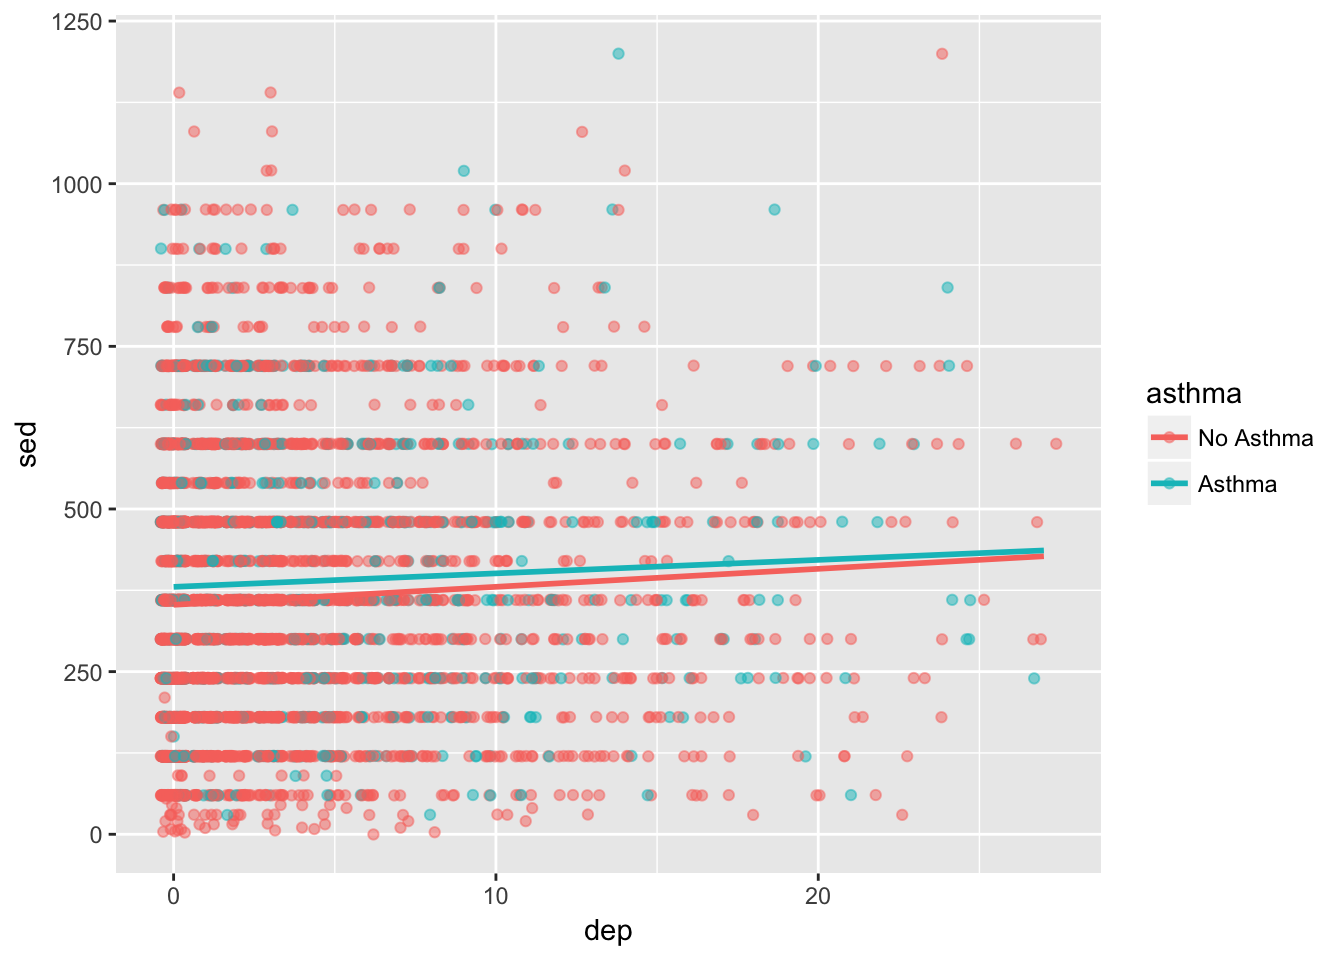
\includegraphics{_main_files/figure-latex/unnamed-chunk-137-1}

This plot is, at best, mediocre. But there's more we can do.

\begin{Shaded}
\begin{Highlighting}[]
\KeywordTok{ggplot}\NormalTok{(df, }\KeywordTok{aes}\NormalTok{(}\DataTypeTok{x =} \KeywordTok{factor}\NormalTok{(dep2), }\DataTypeTok{y =} \KeywordTok{jitter}\NormalTok{(sed, }
    \DecValTok{100}\NormalTok{))) }\OperatorTok{+}\StringTok{ }\KeywordTok{geom_jitter}\NormalTok{(}\DataTypeTok{alpha =} \FloatTok{0.1}\NormalTok{, }\DataTypeTok{color =} \StringTok{"chartreuse4"}\NormalTok{) }\OperatorTok{+}\StringTok{ }
\StringTok{    }\KeywordTok{geom_boxplot}\NormalTok{(}\DataTypeTok{alpha =} \FloatTok{0.75}\NormalTok{, }\DataTypeTok{color =} \StringTok{"dodgerblue4"}\NormalTok{)}
\end{Highlighting}
\end{Shaded}

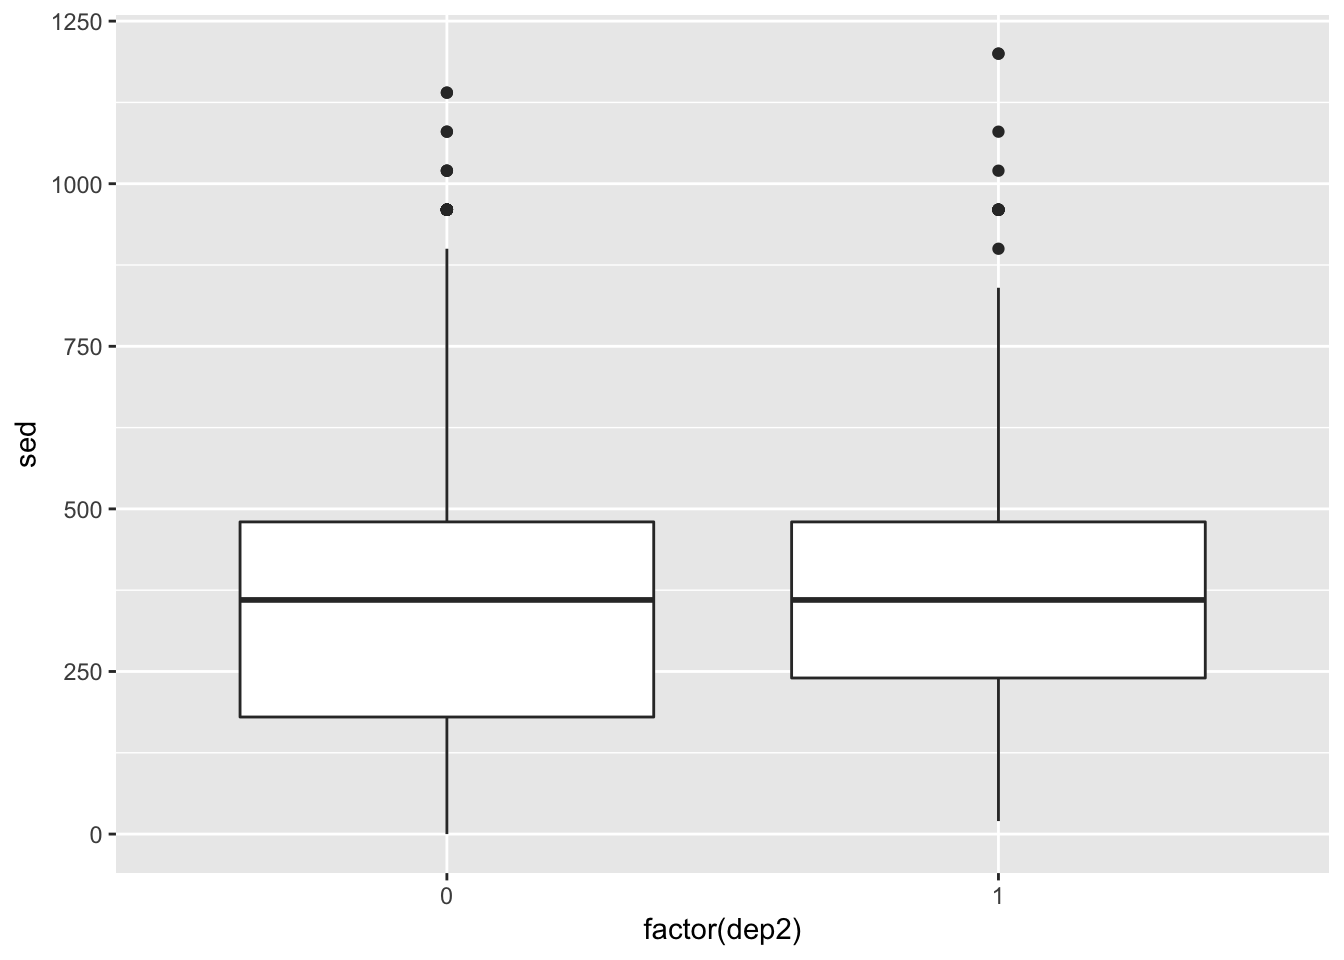
\includegraphics{_main_files/figure-latex/unnamed-chunk-138-1}

This now provides the (jittered) raw data points as well to hightlight
the noise and the number of observations in each group.

\subsection*{Bar Plots}\label{bar-plots}
\addcontentsline{toc}{subsection}{Bar Plots}

Bar plots are great ways to look at means and standard deviations for
groups.

\begin{Shaded}
\begin{Highlighting}[]
\KeywordTok{ggplot}\NormalTok{(summed_data, }\KeywordTok{aes}\NormalTok{(}\DataTypeTok{x =}\NormalTok{ dep2, }\DataTypeTok{y =}\NormalTok{ sed, }\DataTypeTok{group =}\NormalTok{ asthma)) }\OperatorTok{+}\StringTok{ }
\StringTok{    }\KeywordTok{geom_bar}\NormalTok{(}\KeywordTok{aes}\NormalTok{(}\DataTypeTok{fill =}\NormalTok{ asthma), }\DataTypeTok{stat =} \StringTok{"identity"}\NormalTok{, }
        \DataTypeTok{position =} \StringTok{"dodge"}\NormalTok{)}
\end{Highlighting}
\end{Shaded}

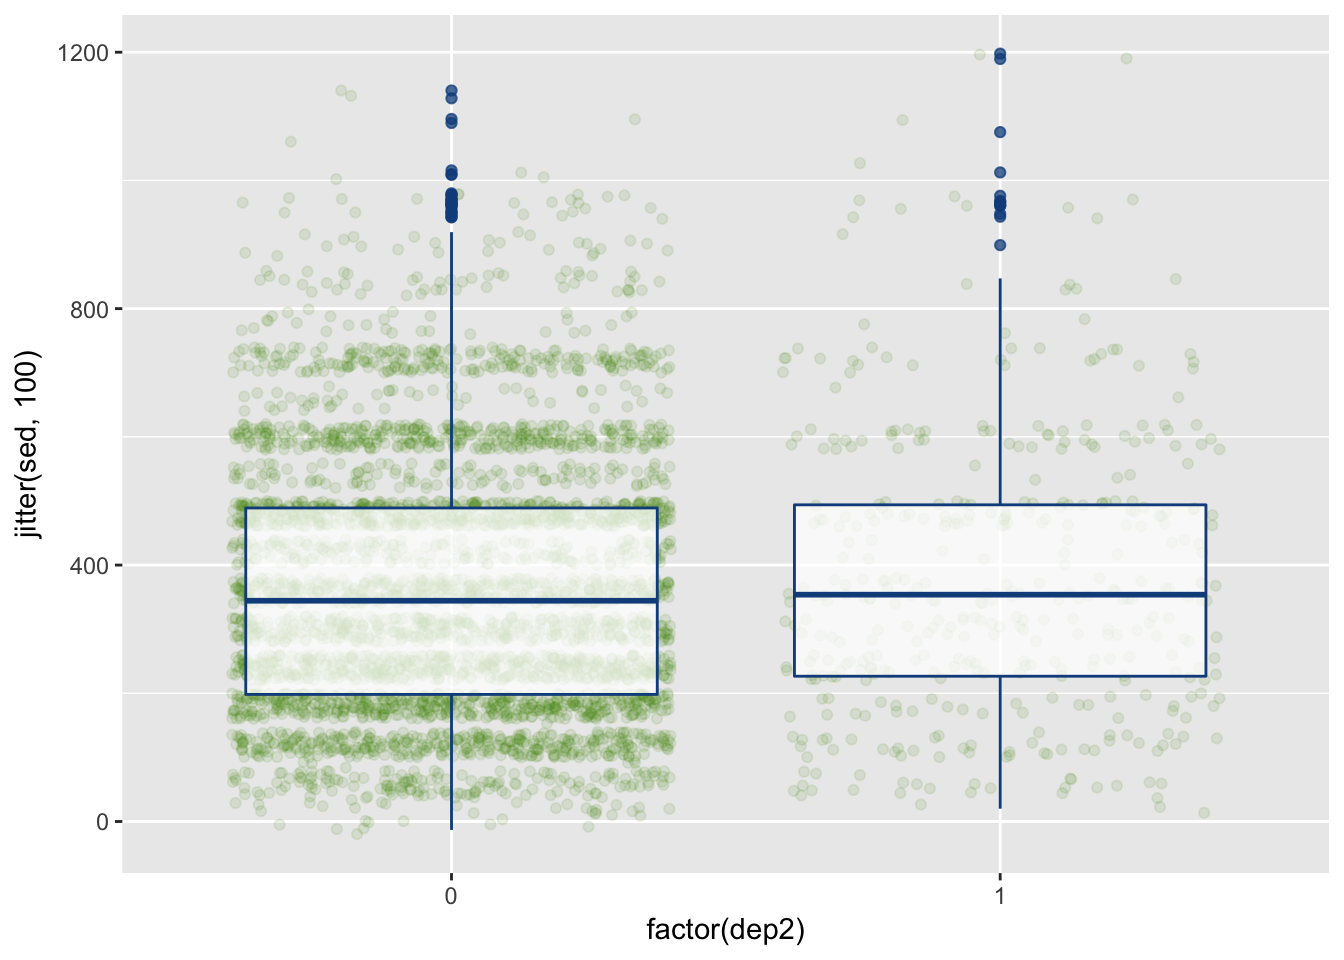
\includegraphics{_main_files/figure-latex/unnamed-chunk-139-1}

We used \texttt{stat\ =\ "identity"} to make it based on the mean
(default is \texttt{count}), and \texttt{position\ =\ "dodge"} makes it
so the bars are next to each other as opposed to stacked. Let's also add
error bars.

\begin{Shaded}
\begin{Highlighting}[]
\NormalTok{p =}\StringTok{ }\KeywordTok{position_dodge}\NormalTok{(}\DataTypeTok{width =} \FloatTok{0.9}\NormalTok{)}
\KeywordTok{ggplot}\NormalTok{(summed_data, }\KeywordTok{aes}\NormalTok{(}\DataTypeTok{x =}\NormalTok{ dep2, }\DataTypeTok{y =}\NormalTok{ sed, }\DataTypeTok{group =}\NormalTok{ asthma)) }\OperatorTok{+}\StringTok{ }
\StringTok{    }\KeywordTok{geom_bar}\NormalTok{(}\KeywordTok{aes}\NormalTok{(}\DataTypeTok{fill =}\NormalTok{ asthma), }\DataTypeTok{stat =} \StringTok{"identity"}\NormalTok{, }
        \DataTypeTok{position =}\NormalTok{ p, }\DataTypeTok{alpha =} \FloatTok{0.8}\NormalTok{) }\OperatorTok{+}\StringTok{ }\KeywordTok{geom_errorbar}\NormalTok{(}\KeywordTok{aes}\NormalTok{(}\DataTypeTok{ymin =}\NormalTok{ sed }\OperatorTok{-}\StringTok{ }
\StringTok{    }\NormalTok{s_se, }\DataTypeTok{ymax =}\NormalTok{ sed }\OperatorTok{+}\StringTok{ }\NormalTok{s_se, }\DataTypeTok{color =}\NormalTok{ asthma), }
    \DataTypeTok{position =}\NormalTok{ p, }\DataTypeTok{width =} \FloatTok{0.3}\NormalTok{)}
\end{Highlighting}
\end{Shaded}

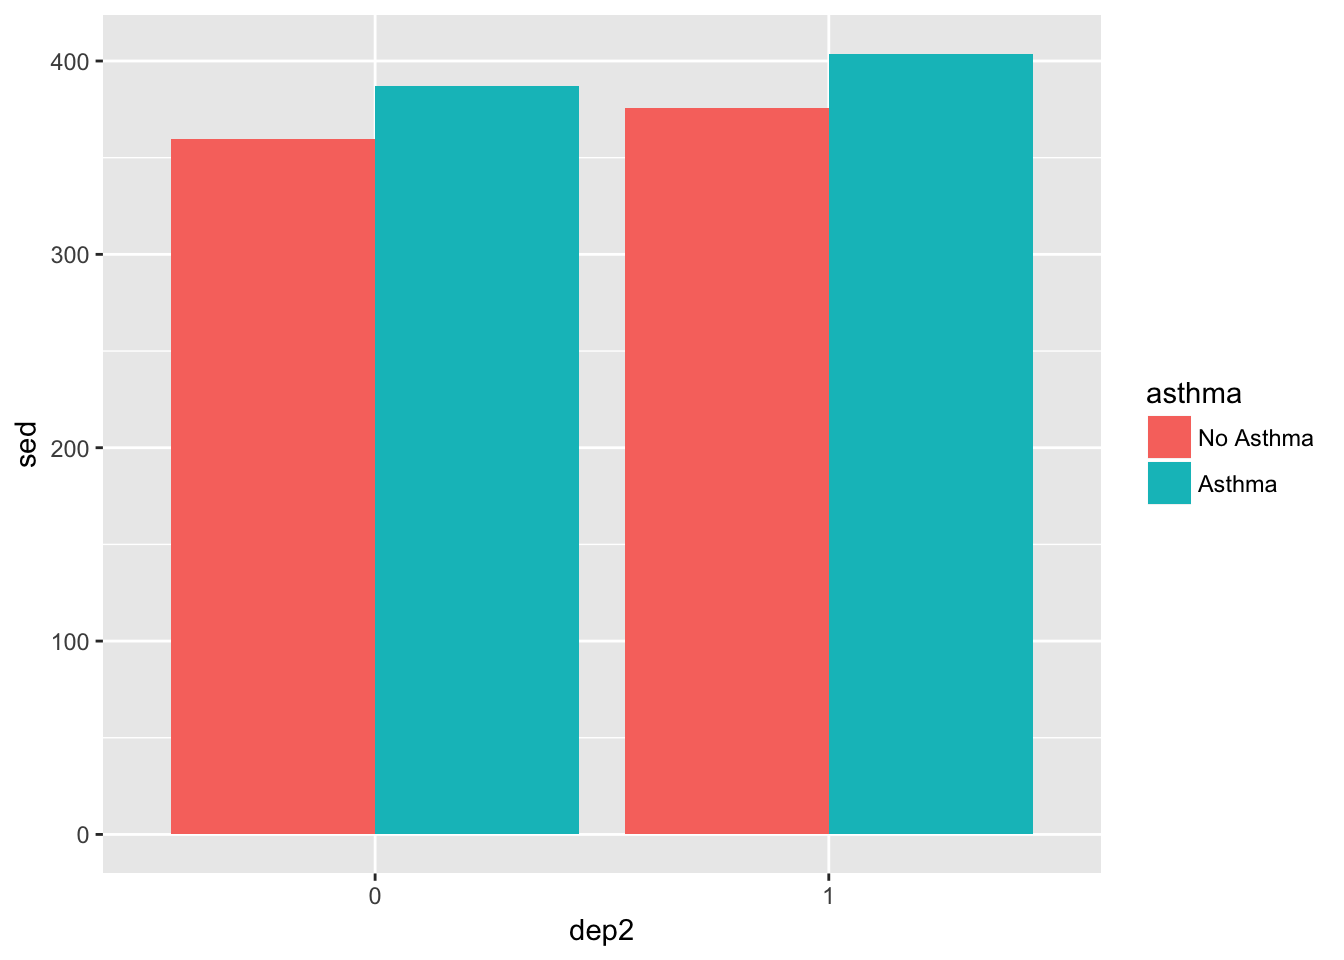
\includegraphics{_main_files/figure-latex/unnamed-chunk-140-1}

There's a lot in there but much of it is what you've seen before. For
example, we use \texttt{alpha} in the \texttt{geom\_bar()} to tell it to
be slightly transparent so we can see the error bars better. We used the
\texttt{position\_dodge()} function to specify exactly how much dodge we
wanted. In this way, we are able to line up the error bars and the bars.
If we just use \texttt{position\ =\ "dodge"} we have less flexibility
and control.

Much more can be done to clean this up, which we'll show in later
sections.

\subsection*{Line Plots}\label{line-plots}
\addcontentsline{toc}{subsection}{Line Plots}

Line plots are particularly good at showing trends and relationships.
Below we we use it to highlight the relationship between depression,
sedentary behavior, and asthma.

\begin{Shaded}
\begin{Highlighting}[]
\KeywordTok{ggplot}\NormalTok{(summed_data, }\KeywordTok{aes}\NormalTok{(}\DataTypeTok{x =}\NormalTok{ dep2, }\DataTypeTok{y =}\NormalTok{ sed, }\DataTypeTok{group =}\NormalTok{ asthma)) }\OperatorTok{+}\StringTok{ }
\StringTok{    }\KeywordTok{geom_line}\NormalTok{(}\KeywordTok{aes}\NormalTok{(}\DataTypeTok{color =}\NormalTok{ asthma))}
\end{Highlighting}
\end{Shaded}

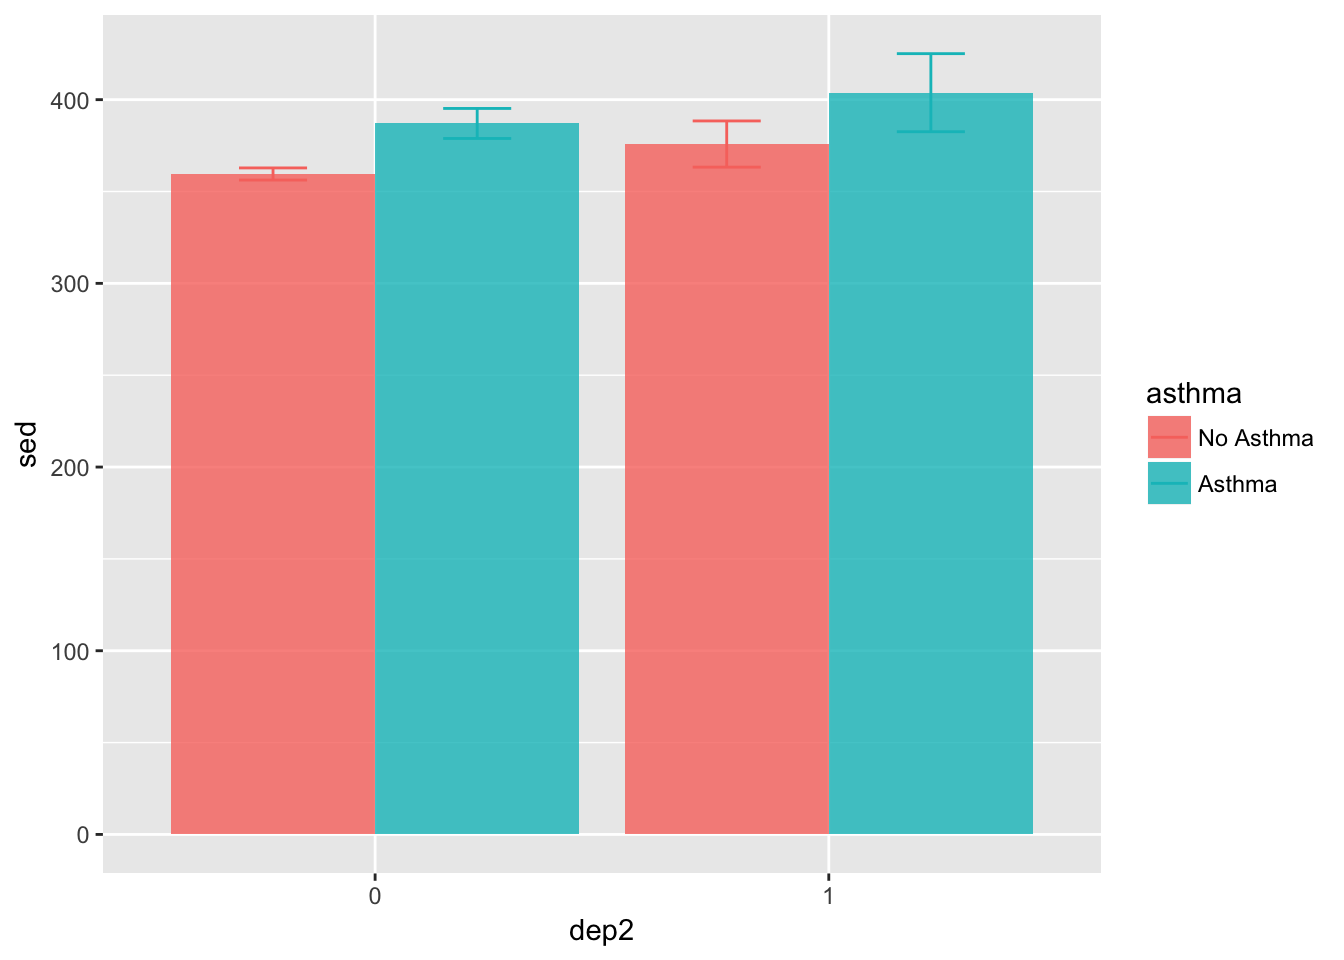
\includegraphics{_main_files/figure-latex/unnamed-chunk-141-1}

Good start, but let's add some features.

\begin{Shaded}
\begin{Highlighting}[]
\NormalTok{pos =}\StringTok{ }\KeywordTok{position_dodge}\NormalTok{(}\DataTypeTok{width =} \FloatTok{0.1}\NormalTok{)}
\KeywordTok{ggplot}\NormalTok{(summed_data, }\KeywordTok{aes}\NormalTok{(}\DataTypeTok{x =}\NormalTok{ dep2, }\DataTypeTok{y =}\NormalTok{ sed, }\DataTypeTok{group =}\NormalTok{ asthma, }
    \DataTypeTok{color =}\NormalTok{ asthma)) }\OperatorTok{+}\StringTok{ }\KeywordTok{geom_line}\NormalTok{(}\DataTypeTok{position =}\NormalTok{ pos) }\OperatorTok{+}\StringTok{ }
\StringTok{    }\KeywordTok{geom_point}\NormalTok{(}\DataTypeTok{position =}\NormalTok{ pos) }\OperatorTok{+}\StringTok{ }\KeywordTok{geom_errorbar}\NormalTok{(}\KeywordTok{aes}\NormalTok{(}\DataTypeTok{ymin =}\NormalTok{ sed }\OperatorTok{-}\StringTok{ }
\StringTok{    }\NormalTok{s_se, }\DataTypeTok{ymax =}\NormalTok{ sed }\OperatorTok{+}\StringTok{ }\NormalTok{s_se), }\DataTypeTok{width =} \FloatTok{0.1}\NormalTok{, }\DataTypeTok{position =}\NormalTok{ pos)}
\end{Highlighting}
\end{Shaded}

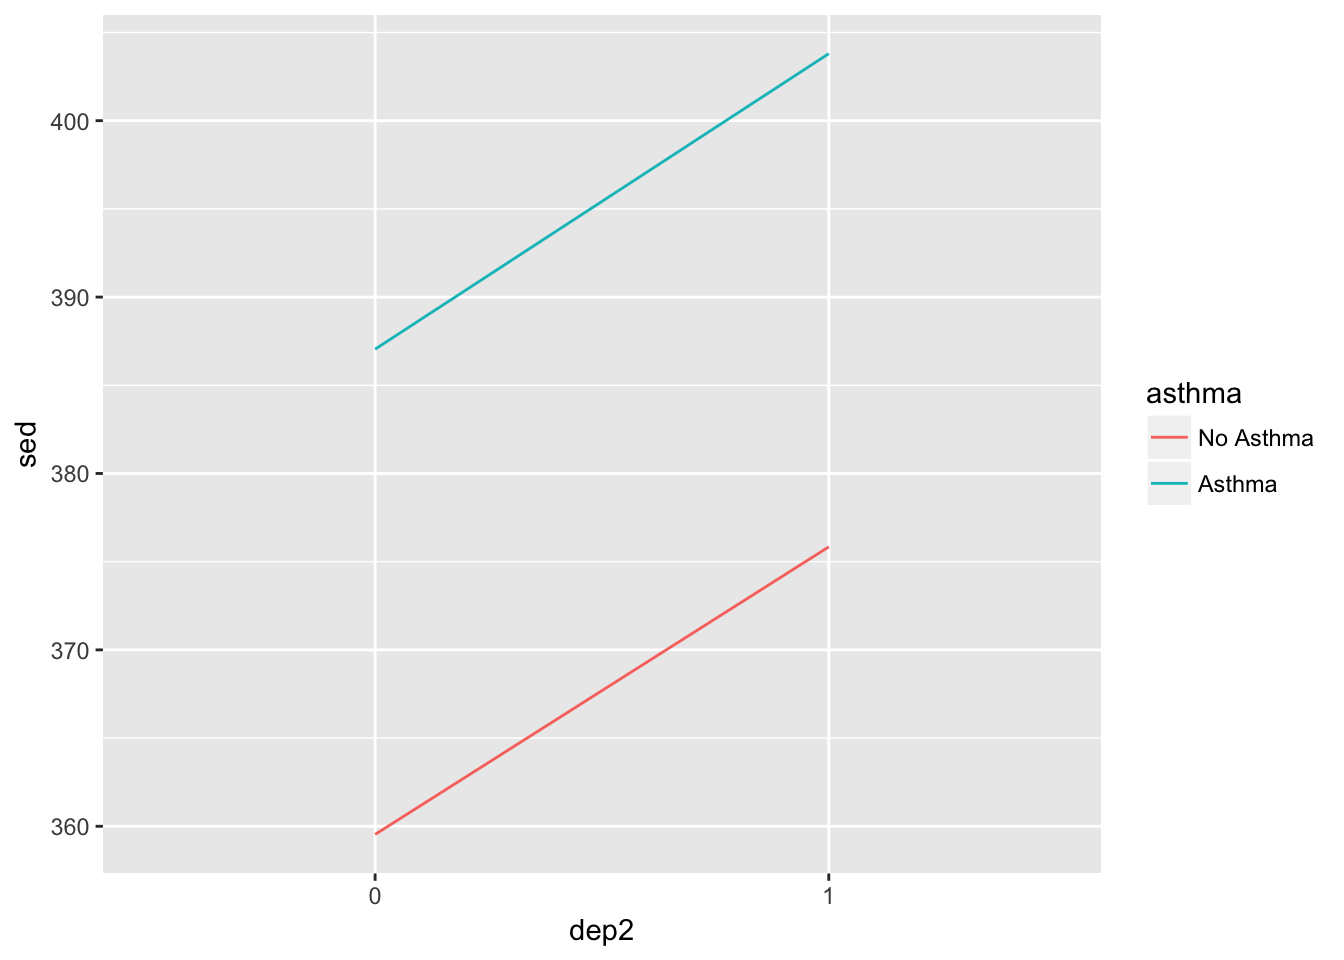
\includegraphics{_main_files/figure-latex/unnamed-chunk-142-1}

That looks a bit better. From here, let's go on to color schemes to make
the plots a bit better.

\section*{Color Schemes}\label{color-schemes}
\addcontentsline{toc}{section}{Color Schemes}

We'll start by using the scatterplot we made above but we will change
the colors a bit using \texttt{scale\_color\_manual()}.

\begin{Shaded}
\begin{Highlighting}[]
\KeywordTok{ggplot}\NormalTok{(df, }\KeywordTok{aes}\NormalTok{(}\DataTypeTok{x =}\NormalTok{ dep, }\DataTypeTok{y =}\NormalTok{ sed, }\DataTypeTok{group =}\NormalTok{ asthma)) }\OperatorTok{+}\StringTok{ }
\StringTok{    }\KeywordTok{geom_jitter}\NormalTok{(}\KeywordTok{aes}\NormalTok{(}\DataTypeTok{color =}\NormalTok{ asthma), }\DataTypeTok{alpha =} \FloatTok{0.5}\NormalTok{) }\OperatorTok{+}\StringTok{ }
\StringTok{    }\KeywordTok{geom_smooth}\NormalTok{(}\KeywordTok{aes}\NormalTok{(}\DataTypeTok{color =}\NormalTok{ asthma), }\DataTypeTok{method =} \StringTok{"lm"}\NormalTok{, }
        \DataTypeTok{se =} \OtherTok{FALSE}\NormalTok{) }\OperatorTok{+}\StringTok{ }\KeywordTok{scale_color_manual}\NormalTok{(}\DataTypeTok{values =} \KeywordTok{c}\NormalTok{(}\StringTok{"dodgerblue4"}\NormalTok{, }
    \StringTok{"chartreuse4"}\NormalTok{))}
\end{Highlighting}
\end{Shaded}

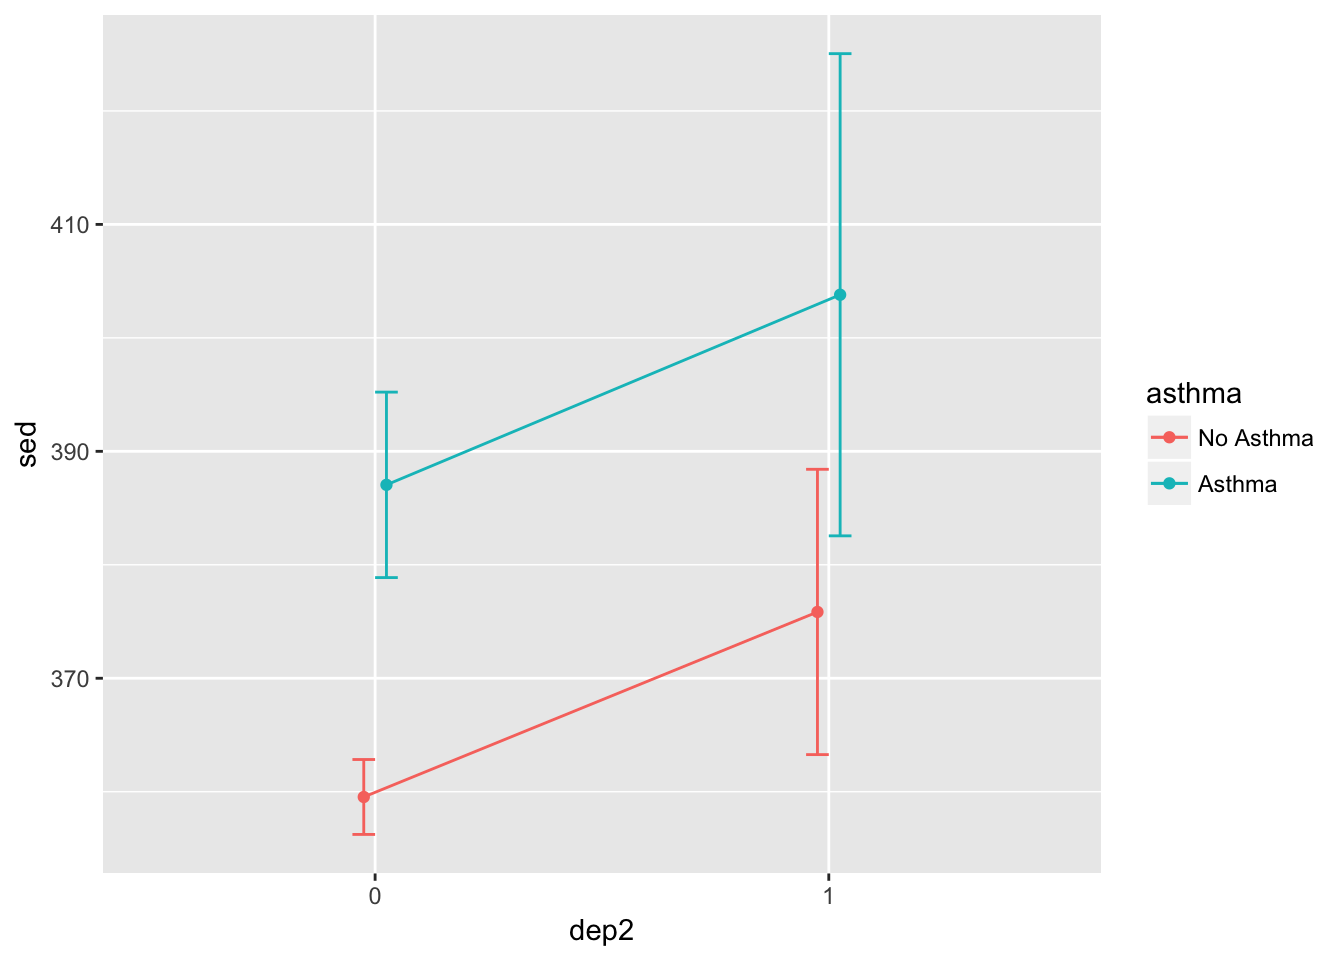
\includegraphics{_main_files/figure-latex/unnamed-chunk-143-1} Depending
on your personal taste, you can adjust it with any color. On my blog,
I've \href{https:/tysonstanley.github.io}{posted} the colors available
in R (there are many).

\begin{quote}
Advice: Don't get too lost in selecting colors but it can add a nice
touch to any plot. The nuances of plot design can be invigorating but
also time consuming to be smart about how long you spend using it.
\end{quote}

Next, let's adjust the bar plot. We will also add some colors here, but
we will differentiate between ``color'' and ``fill''.

\begin{enumerate}
\def\labelenumi{\arabic{enumi}.}
\tightlist
\item
  Fill fills in the object with color. This is useful for things that
  are more than simply a line or a dot.
\item
  Color colors the object. This outlines those items that can also be
  filled and colors lines and dots.
\end{enumerate}

\begin{Shaded}
\begin{Highlighting}[]
\NormalTok{p =}\StringTok{ }\KeywordTok{position_dodge}\NormalTok{(}\DataTypeTok{width =}\NormalTok{ .}\DecValTok{9}\NormalTok{)}
\KeywordTok{ggplot}\NormalTok{(summed_data, }\KeywordTok{aes}\NormalTok{(}\DataTypeTok{x =}\NormalTok{ dep2, }\DataTypeTok{y =}\NormalTok{ sed, }\DataTypeTok{group =}\NormalTok{ asthma)) }\OperatorTok{+}
\StringTok{  }\KeywordTok{geom_bar}\NormalTok{(}\KeywordTok{aes}\NormalTok{(}\DataTypeTok{fill =}\NormalTok{ asthma, }\DataTypeTok{color =}\NormalTok{ asthma), }
           \DataTypeTok{stat =} \StringTok{"identity"}\NormalTok{, }
           \DataTypeTok{position =}\NormalTok{ p,}
           \DataTypeTok{alpha =}\NormalTok{ .}\DecValTok{8}\NormalTok{) }\OperatorTok{+}
\StringTok{  }\KeywordTok{geom_errorbar}\NormalTok{(}\KeywordTok{aes}\NormalTok{(}\DataTypeTok{ymin =}\NormalTok{ sed }\OperatorTok{-}\StringTok{ }\NormalTok{s_se, }\DataTypeTok{ymax =}\NormalTok{ sed }\OperatorTok{+}\StringTok{ }\NormalTok{s_se,}
                    \DataTypeTok{color =}\NormalTok{ asthma), }
                \DataTypeTok{position =}\NormalTok{ p,}
                \DataTypeTok{width =}\NormalTok{ .}\DecValTok{3}\NormalTok{) }\OperatorTok{+}
\StringTok{  }\KeywordTok{scale_color_manual}\NormalTok{(}\DataTypeTok{values =} \KeywordTok{c}\NormalTok{(}\StringTok{"dodgerblue4"}\NormalTok{, }\StringTok{"chartreuse4"}\NormalTok{)) }\OperatorTok{+}\StringTok{   }\NormalTok{## controls the color of the error bars}
\StringTok{  }\KeywordTok{scale_fill_manual}\NormalTok{(}\DataTypeTok{values =} \KeywordTok{c}\NormalTok{(}\StringTok{"aliceblue"}\NormalTok{, }\StringTok{"beige"}\NormalTok{))}
\end{Highlighting}
\end{Shaded}

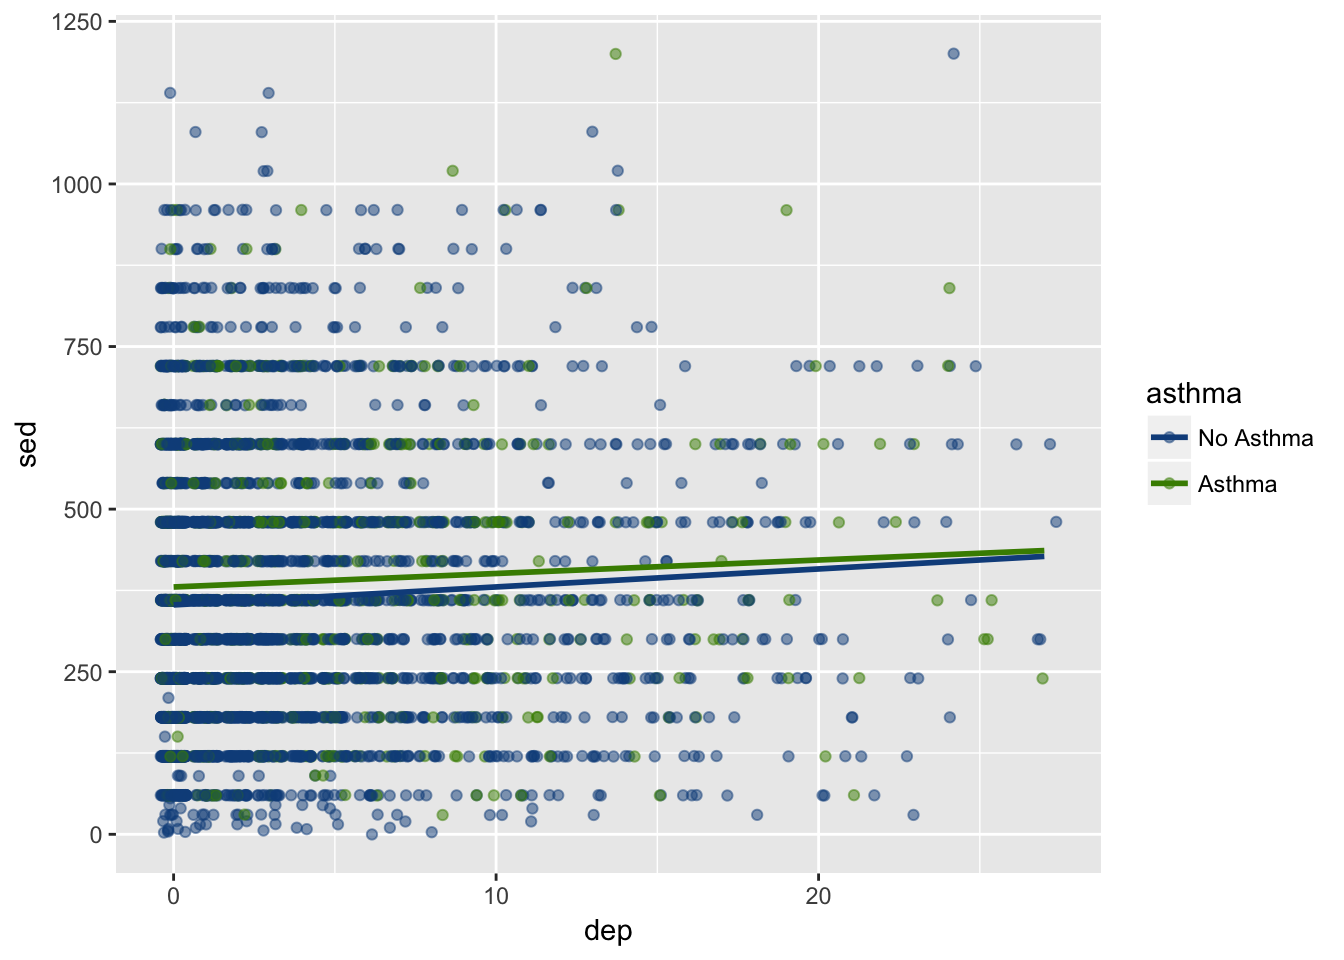
\includegraphics{_main_files/figure-latex/unnamed-chunk-144-1}

Just so you are aware:

\begin{itemize}
\tightlist
\item
  aliceblue is a lightblue
\item
  beige is a light green
\item
  dodgerblue4 is a dark blue
\item
  chartreuse4 is a dark green
\end{itemize}

So the \texttt{fill} colors are light and the \texttt{color} colors are
dark in this example. You, of course, can do whatever you want
color-wise. I'm a fan of this style though so we will keep it for now.

These same functions can be used on the other plots as well. Feel free
to give them a try. As for the book, we'll move on to the next section:
Themes.

\section*{Themes}\label{themes}
\addcontentsline{toc}{section}{Themes}

Using the plot we just made--the bar plot--we will show how theme
options work. There are several built in themes that change many aspects
of the plot (e.g., \texttt{theme\_bw()}, \texttt{theme\_classic()},
\texttt{theme\_minimal()}). There are many more if you download the
\texttt{ggthemes} package. Fairly simply you can create plots similar to
those in newspapers and magazines.

First, we are going to save the plot to simply show the different
theming options.

\begin{Shaded}
\begin{Highlighting}[]
\NormalTok{p =}\StringTok{ }\KeywordTok{position_dodge}\NormalTok{(}\DataTypeTok{width =}\NormalTok{ .}\DecValTok{9}\NormalTok{)}
\NormalTok{p1 =}\StringTok{ }\KeywordTok{ggplot}\NormalTok{(summed_data, }\KeywordTok{aes}\NormalTok{(}\DataTypeTok{x =}\NormalTok{ dep2, }\DataTypeTok{y =}\NormalTok{ sed, }\DataTypeTok{group =}\NormalTok{ asthma)) }\OperatorTok{+}
\StringTok{  }\KeywordTok{geom_bar}\NormalTok{(}\KeywordTok{aes}\NormalTok{(}\DataTypeTok{fill =}\NormalTok{ asthma, }\DataTypeTok{color =}\NormalTok{ asthma), }
           \DataTypeTok{stat =} \StringTok{"identity"}\NormalTok{, }
           \DataTypeTok{position =}\NormalTok{ p,}
           \DataTypeTok{alpha =}\NormalTok{ .}\DecValTok{8}\NormalTok{) }\OperatorTok{+}
\StringTok{  }\KeywordTok{geom_errorbar}\NormalTok{(}\KeywordTok{aes}\NormalTok{(}\DataTypeTok{ymin =}\NormalTok{ sed }\OperatorTok{-}\StringTok{ }\NormalTok{s_se, }\DataTypeTok{ymax =}\NormalTok{ sed }\OperatorTok{+}\StringTok{ }\NormalTok{s_se,}
                    \DataTypeTok{color =}\NormalTok{ asthma), }
                \DataTypeTok{position =}\NormalTok{ p,}
                \DataTypeTok{width =}\NormalTok{ .}\DecValTok{3}\NormalTok{) }\OperatorTok{+}
\StringTok{  }\KeywordTok{scale_color_manual}\NormalTok{(}\DataTypeTok{values =} \KeywordTok{c}\NormalTok{(}\StringTok{"dodgerblue4"}\NormalTok{, }\StringTok{"chartreuse4"}\NormalTok{)) }\OperatorTok{+}\StringTok{   }\NormalTok{## controls the color of the error bars}
\StringTok{  }\KeywordTok{scale_fill_manual}\NormalTok{(}\DataTypeTok{values =} \KeywordTok{c}\NormalTok{(}\StringTok{"aliceblue"}\NormalTok{, }\StringTok{"beige"}\NormalTok{))}
\end{Highlighting}
\end{Shaded}

\subsubsection*{Theme Black and White}\label{theme-black-and-white}
\addcontentsline{toc}{subsubsection}{Theme Black and White}

\begin{Shaded}
\begin{Highlighting}[]
\NormalTok{p1 }\OperatorTok{+}\StringTok{ }\KeywordTok{theme_bw}\NormalTok{()}
\end{Highlighting}
\end{Shaded}

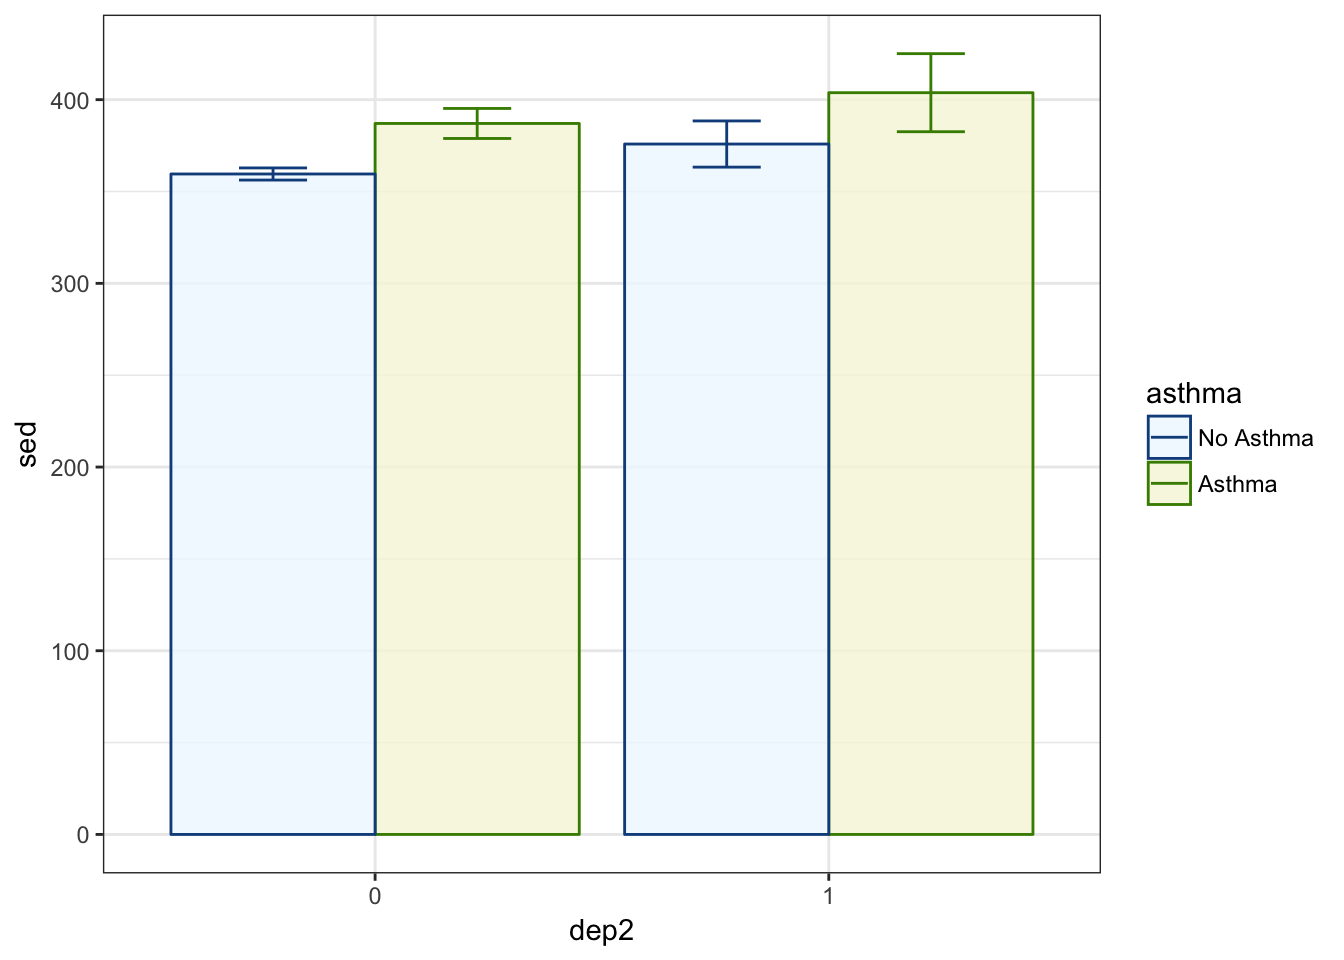
\includegraphics{_main_files/figure-latex/unnamed-chunk-146-1}

\subsubsection*{Theme Classic}\label{theme-classic}
\addcontentsline{toc}{subsubsection}{Theme Classic}

\begin{Shaded}
\begin{Highlighting}[]
\NormalTok{p1 }\OperatorTok{+}\StringTok{ }\KeywordTok{theme_classic}\NormalTok{()}
\end{Highlighting}
\end{Shaded}

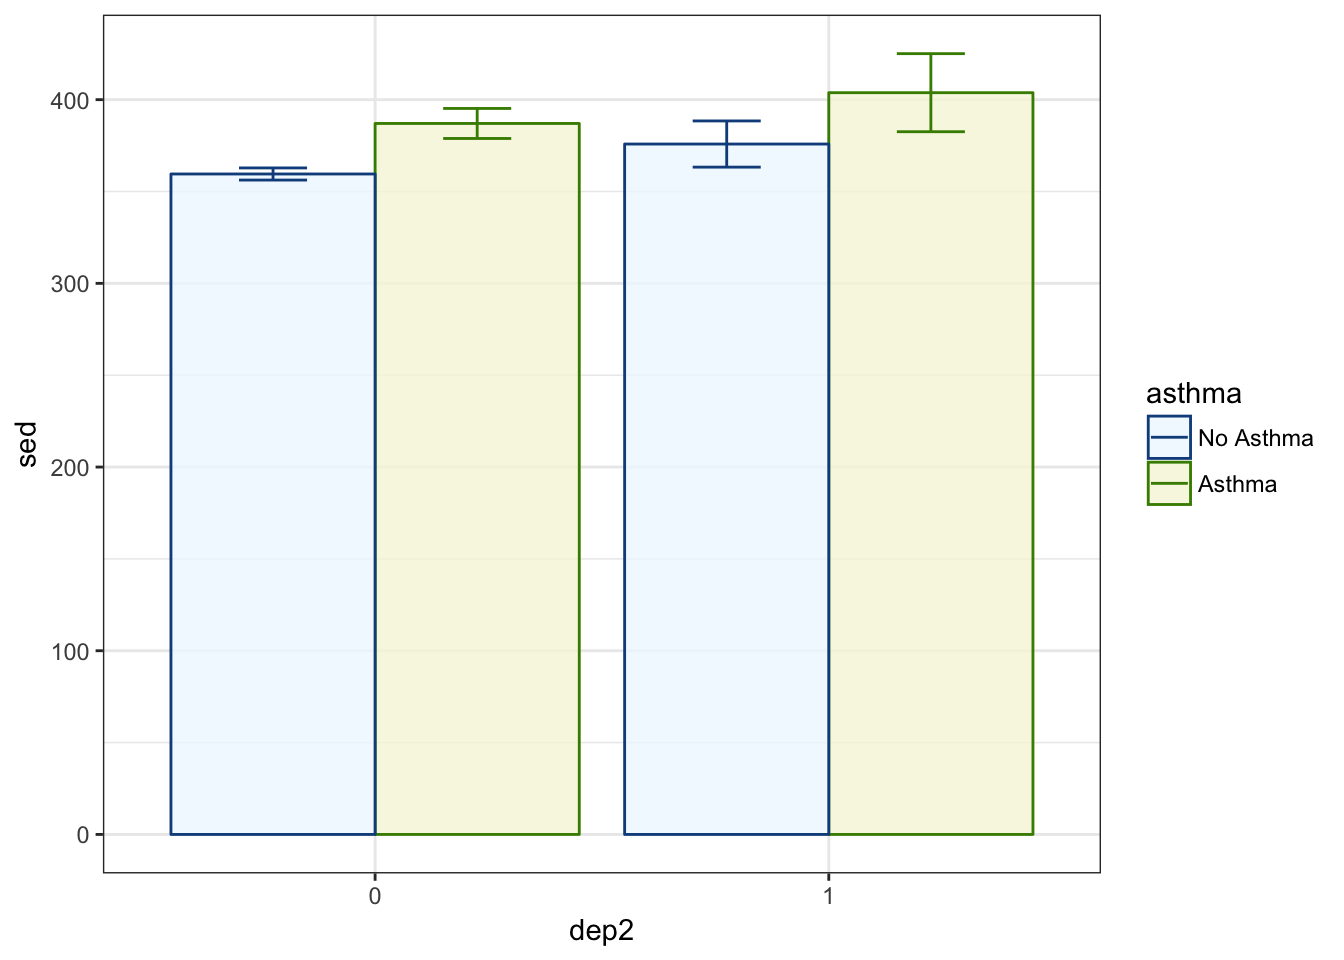
\includegraphics{_main_files/figure-latex/unnamed-chunk-147-1}

\subsubsection*{Theme Minimal}\label{theme-minimal}
\addcontentsline{toc}{subsubsection}{Theme Minimal}

\begin{Shaded}
\begin{Highlighting}[]
\NormalTok{p1 }\OperatorTok{+}\StringTok{ }\KeywordTok{theme_minimal}\NormalTok{()}
\end{Highlighting}
\end{Shaded}

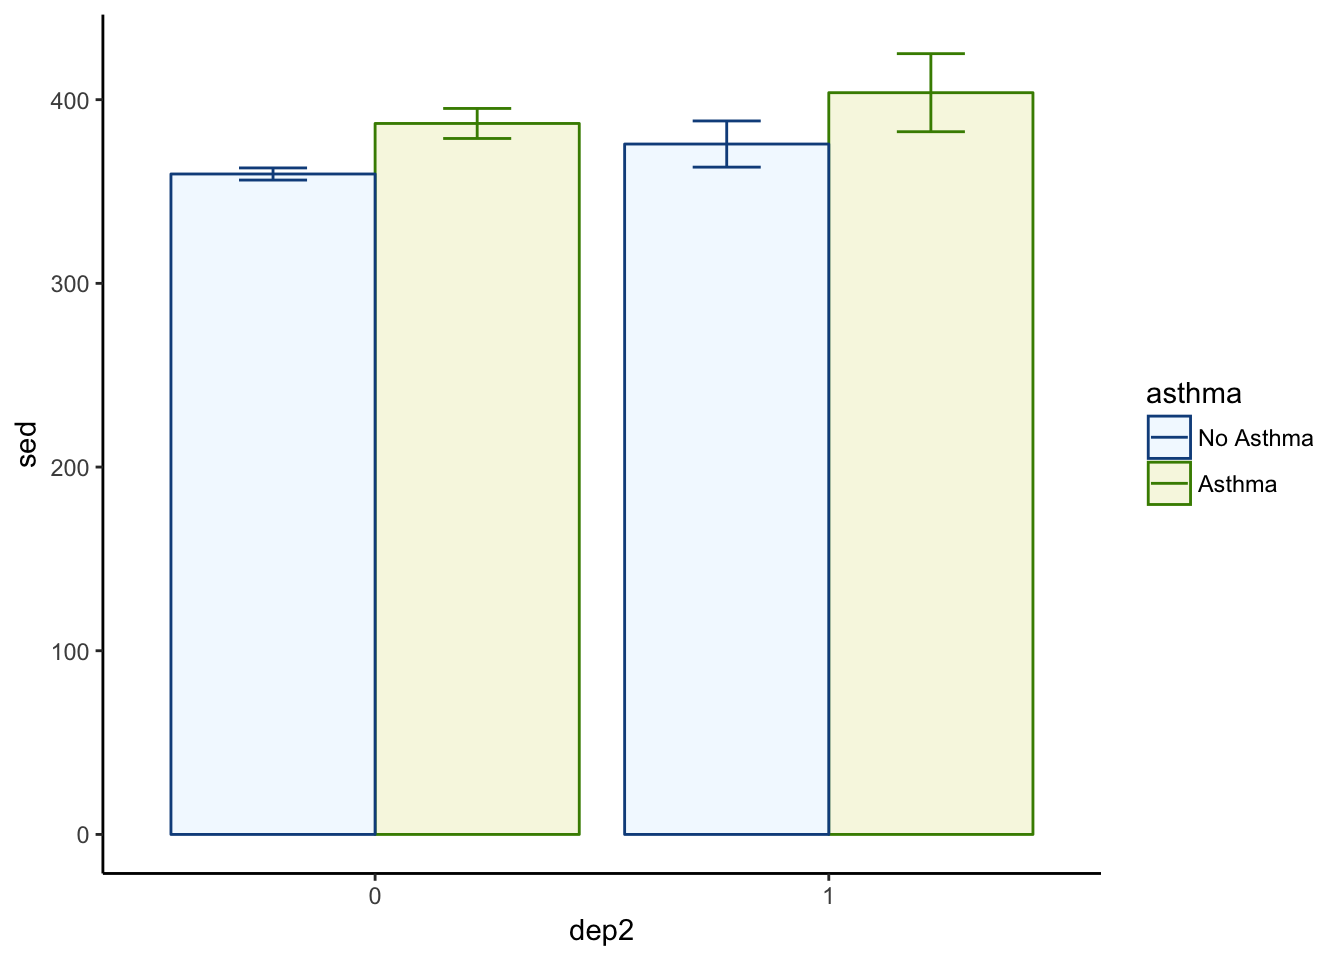
\includegraphics{_main_files/figure-latex/unnamed-chunk-148-1}

\subsubsection*{\texorpdfstring{Theme Economist (from
\texttt{ggthemes})}{Theme Economist (from ggthemes)}}\label{theme-economist-from-ggthemes}
\addcontentsline{toc}{subsubsection}{Theme Economist (from
\texttt{ggthemes})}

\begin{Shaded}
\begin{Highlighting}[]
\KeywordTok{library}\NormalTok{(ggthemes)}
\NormalTok{p1 }\OperatorTok{+}\StringTok{ }\KeywordTok{theme_economist}\NormalTok{()}
\end{Highlighting}
\end{Shaded}

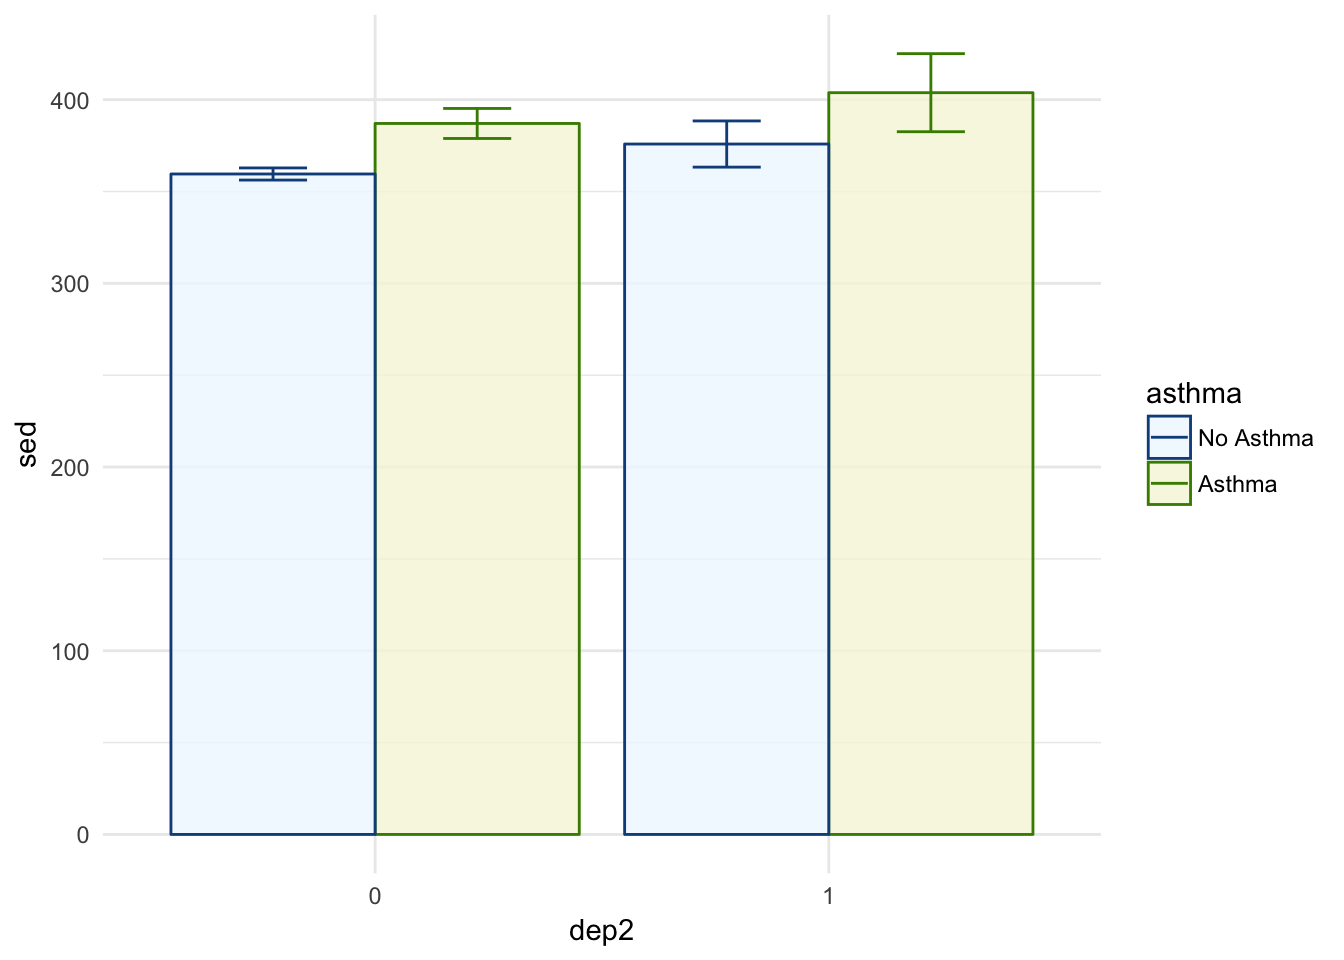
\includegraphics{_main_files/figure-latex/unnamed-chunk-149-1}

\subsubsection*{\texorpdfstring{Theme FiveThirtyEight (from
\texttt{ggthemes})}{Theme FiveThirtyEight (from ggthemes)}}\label{theme-fivethirtyeight-from-ggthemes}
\addcontentsline{toc}{subsubsection}{Theme FiveThirtyEight (from
\texttt{ggthemes})}

\begin{Shaded}
\begin{Highlighting}[]
\NormalTok{p1 }\OperatorTok{+}\StringTok{ }\KeywordTok{theme_fivethirtyeight}\NormalTok{()}
\end{Highlighting}
\end{Shaded}

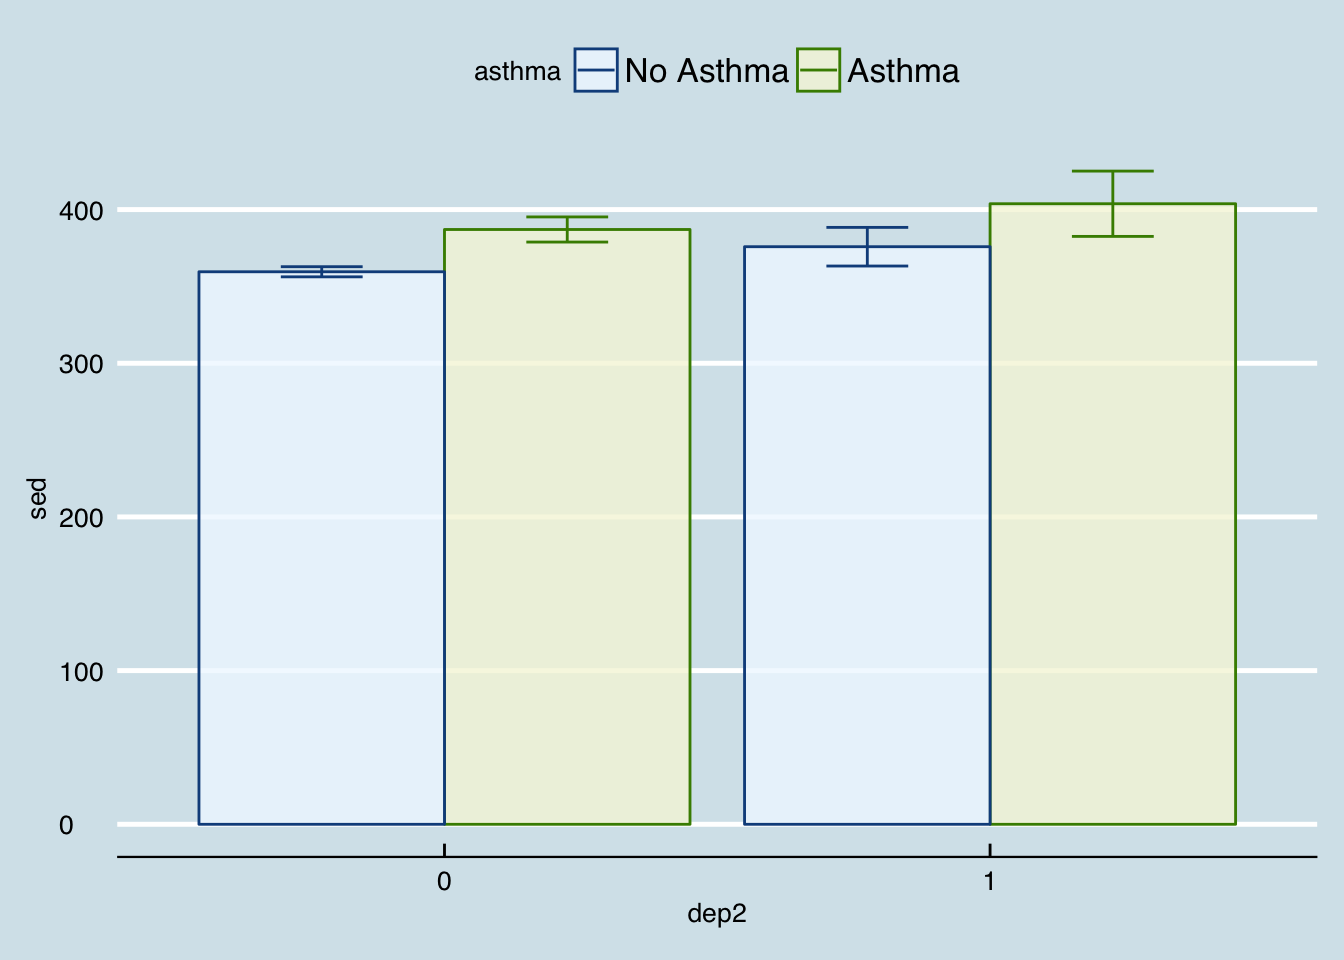
\includegraphics{_main_files/figure-latex/unnamed-chunk-150-1}

\subsubsection*{\texorpdfstring{Theme Tufte (from
\texttt{ggthemes})}{Theme Tufte (from ggthemes)}}\label{theme-tufte-from-ggthemes}
\addcontentsline{toc}{subsubsection}{Theme Tufte (from
\texttt{ggthemes})}

\begin{Shaded}
\begin{Highlighting}[]
\NormalTok{p1 }\OperatorTok{+}\StringTok{ }\KeywordTok{theme_tufte}\NormalTok{()}
\end{Highlighting}
\end{Shaded}

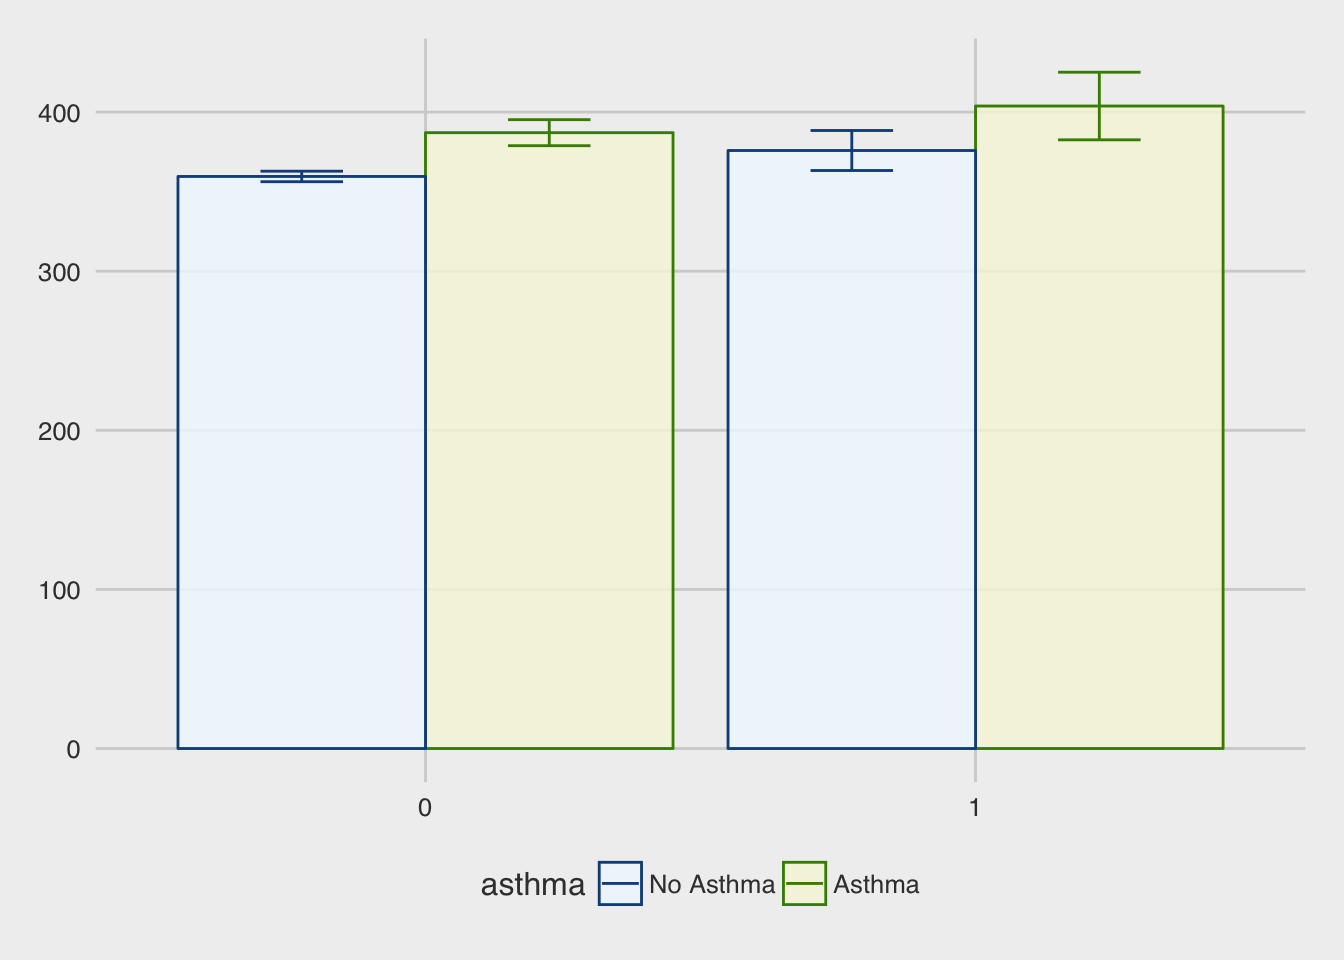
\includegraphics{_main_files/figure-latex/unnamed-chunk-151-1}

\subsubsection*{\texorpdfstring{Theme Stata (from
\texttt{ggthemes})}{Theme Stata (from ggthemes)}}\label{theme-stata-from-ggthemes}
\addcontentsline{toc}{subsubsection}{Theme Stata (from
\texttt{ggthemes})}

\begin{Shaded}
\begin{Highlighting}[]
\NormalTok{p1 }\OperatorTok{+}\StringTok{ }\KeywordTok{theme_stata}\NormalTok{()}
\end{Highlighting}
\end{Shaded}

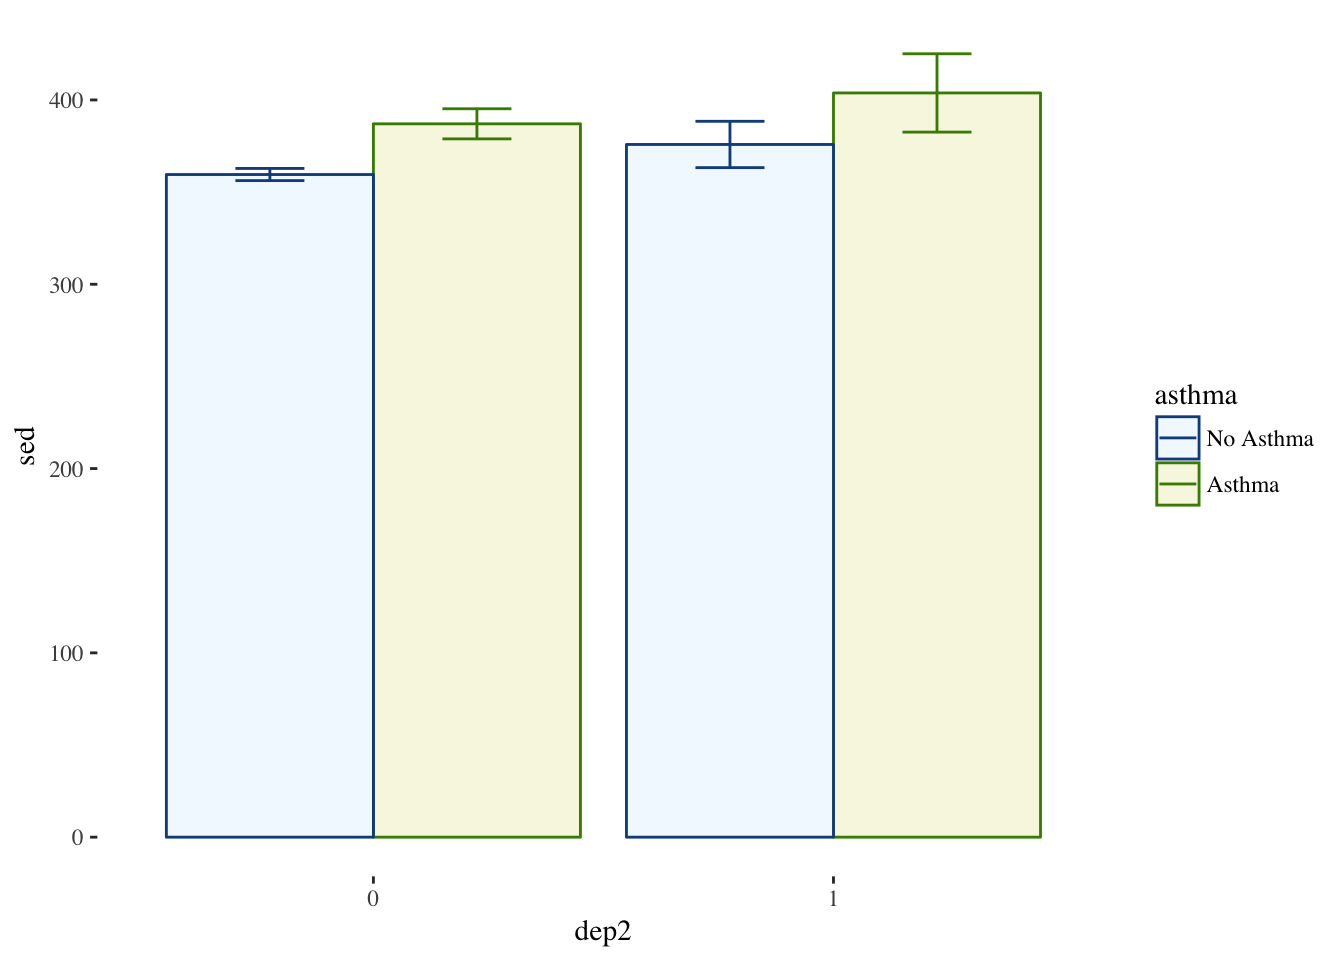
\includegraphics{_main_files/figure-latex/unnamed-chunk-152-1}

\subsubsection*{Your Own Theme}\label{your-own-theme}
\addcontentsline{toc}{subsubsection}{Your Own Theme}

There are many more but you get the idea. In addition to the built in
themes, you can use the \texttt{theme()} function and make your own
adjustments. There are \emph{many} options so we will just introduce the
idea.

\begin{Shaded}
\begin{Highlighting}[]
\NormalTok{p1 }\OperatorTok{+}\StringTok{ }
\StringTok{  }\KeywordTok{theme}\NormalTok{(}\DataTypeTok{legend.position =} \StringTok{"bottom"}\NormalTok{,  ## puts legend at the bottom of figure}
        \DataTypeTok{legend.background =} \KeywordTok{element_rect}\NormalTok{(}\DataTypeTok{color =} \StringTok{"lightgrey"}\NormalTok{),  ## outlines legend}
        \DataTypeTok{panel.background =} \KeywordTok{element_rect}\NormalTok{(}\DataTypeTok{fill =} \StringTok{"grey99"}\NormalTok{,   ## fills the plot with a very light grey}
                                        \DataTypeTok{color =} \StringTok{"grey70"}\NormalTok{),  ## light border around plot}
        \DataTypeTok{text =} \KeywordTok{element_text}\NormalTok{(}\DataTypeTok{family =} \StringTok{"Times"}\NormalTok{))     ## all text in plot is now Times}
\end{Highlighting}
\end{Shaded}

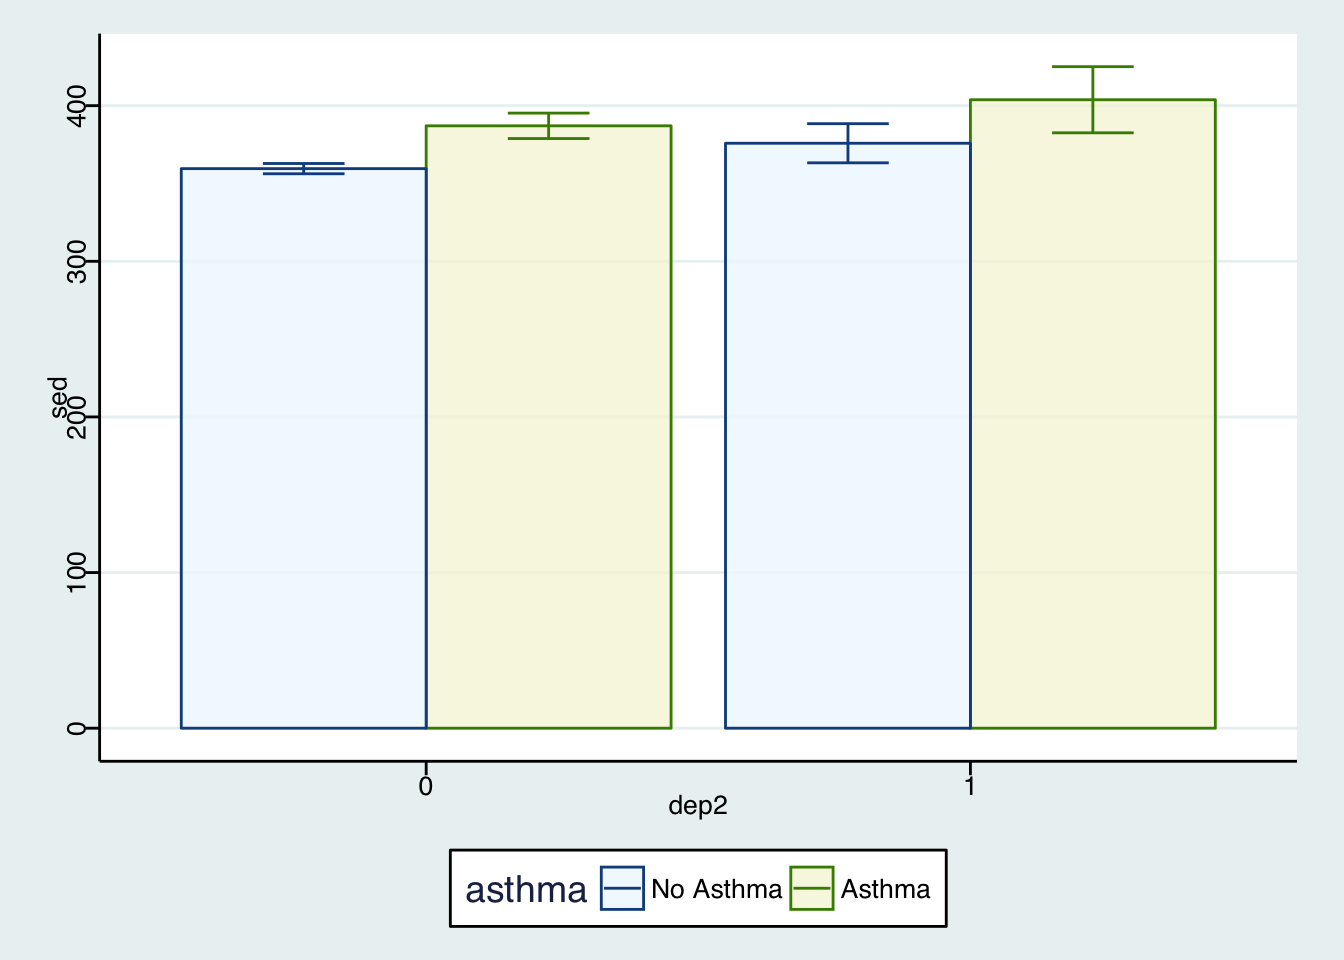
\includegraphics{_main_files/figure-latex/unnamed-chunk-153-1}

There are many more options but essentially if there is something you
want to change, you probably can.

\section*{Labels and Titles}\label{labels-and-titles}
\addcontentsline{toc}{section}{Labels and Titles}

Using our last plot, we will also want to add good labels and/or titles.

\begin{Shaded}
\begin{Highlighting}[]
\NormalTok{p1 }\OperatorTok{+}\StringTok{ }\KeywordTok{theme}\NormalTok{(}\DataTypeTok{legend.position =} \StringTok{"bottom"}\NormalTok{, }\DataTypeTok{legend.background =} \KeywordTok{element_rect}\NormalTok{(}\DataTypeTok{color =} \StringTok{"lightgrey"}\NormalTok{), }
    \DataTypeTok{panel.background =} \KeywordTok{element_rect}\NormalTok{(}\DataTypeTok{fill =} \StringTok{"grey99"}\NormalTok{, }
        \DataTypeTok{color =} \StringTok{"grey70"}\NormalTok{), }\DataTypeTok{text =} \KeywordTok{element_text}\NormalTok{(}\DataTypeTok{family =} \StringTok{"Times"}\NormalTok{)) }\OperatorTok{+}\StringTok{ }
\StringTok{    }\KeywordTok{labs}\NormalTok{(}\DataTypeTok{y =} \StringTok{"Sedentary Behavior (Minutes)"}\NormalTok{, }\DataTypeTok{x =} \StringTok{"Depression (1 = Depressed)"}\NormalTok{, }
        \DataTypeTok{title =} \StringTok{"Comparison of Sedentary Behavior"}\NormalTok{, }
        \DataTypeTok{subtitle =} \StringTok{"across Depression and Asthma"}\NormalTok{)}
\end{Highlighting}
\end{Shaded}

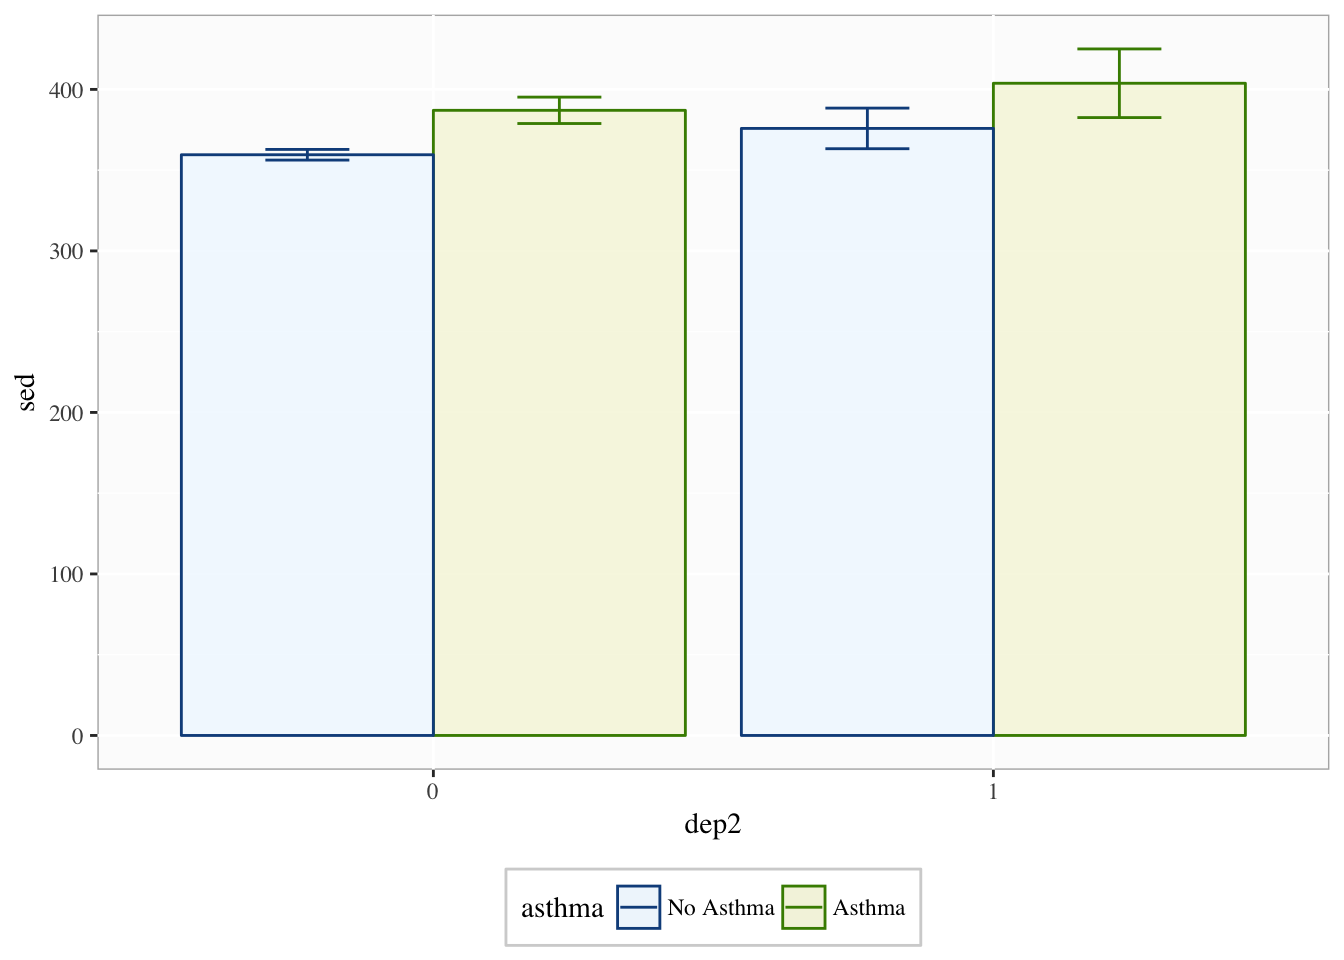
\includegraphics{_main_files/figure-latex/unnamed-chunk-154-1}

\section*{Facetting}\label{facetting}
\addcontentsline{toc}{section}{Facetting}

Facetting is very useful when trying to compare more than three
variables at a time or you cannot use color or shading. It is often
useful and beautiful. Facetting splits the data based on some grouping
variable (e.g., asthma) to highlight differences in the relationship.

\begin{Shaded}
\begin{Highlighting}[]
\NormalTok{p1 }\OperatorTok{+}\StringTok{ }\KeywordTok{theme}\NormalTok{(}\DataTypeTok{legend.position =} \StringTok{"bottom"}\NormalTok{, }\DataTypeTok{legend.background =} \KeywordTok{element_rect}\NormalTok{(}\DataTypeTok{color =} \StringTok{"lightgrey"}\NormalTok{), }
    \DataTypeTok{panel.background =} \KeywordTok{element_rect}\NormalTok{(}\DataTypeTok{fill =} \StringTok{"grey99"}\NormalTok{, }
        \DataTypeTok{color =} \StringTok{"grey70"}\NormalTok{), }\DataTypeTok{text =} \KeywordTok{element_text}\NormalTok{(}\DataTypeTok{family =} \StringTok{"Times"}\NormalTok{)) }\OperatorTok{+}\StringTok{ }
\StringTok{    }\KeywordTok{labs}\NormalTok{(}\DataTypeTok{y =} \StringTok{"Sedentary Behavior (Minutes)"}\NormalTok{, }\DataTypeTok{x =} \StringTok{"Depression (1 = Depressed)"}\NormalTok{, }
        \DataTypeTok{title =} \StringTok{"Comparison of Sedentary Behavior"}\NormalTok{, }
        \DataTypeTok{subtitle =} \StringTok{"across Depression and Asthma"}\NormalTok{) }\OperatorTok{+}\StringTok{ }
\StringTok{    }\KeywordTok{facet_grid}\NormalTok{(}\OperatorTok{~}\NormalTok{asthma)}
\end{Highlighting}
\end{Shaded}

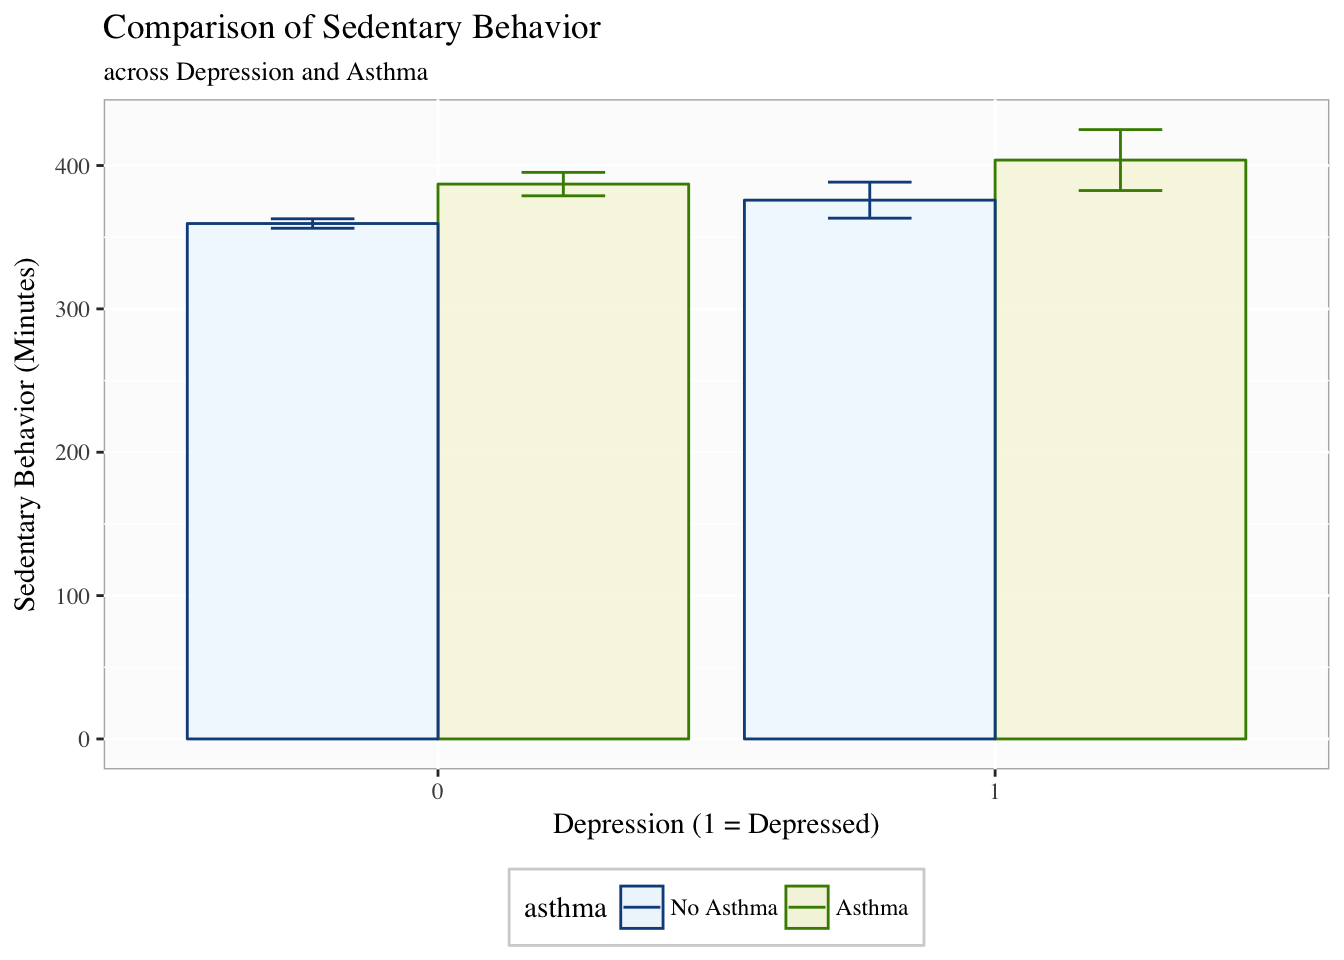
\includegraphics{_main_files/figure-latex/unnamed-chunk-155-1}

You can facet by more than one variable and it will create separate
panels for each combination of the facetting variables.

\section*{Conclusions}\label{conclusions-5}
\addcontentsline{toc}{section}{Conclusions}

This was a quick demonstration of plotting with \texttt{ggplot2}. There
is so much more you can do. However, in the end, exploring and
communicating the data through plots is simply something you need to
practice. With time, you can \emph{a priori} picture the types of plots
that will highlight things in your data, the ways you can adjust it, and
how you need to manipulate your data to make it plot ready. Be patient
and have fun trying things. In my experience, almost anytime I think,
``Can R do this?'', it can, so try to do cool stuff and you'll probably
find that you can.

\chapter*{Chapter 10: Where to Go from Here and Common
Pitfalls}\label{chapter-10-where-to-go-from-here-and-common-pitfalls}
\addcontentsline{toc}{chapter}{Chapter 10: Where to Go from Here and
Common Pitfalls}

\begin{quote}
``The journey of a thousand miles begins with one step.''

--- Lao Tzu
\end{quote}

There are many resources that can aid in developing your \texttt{R}
skills from here. We have introduced the basics of \texttt{R}, helping
you take a few steps on your journey of understanding \texttt{R}. We
have focused on the ones that are most important for researchers in the
health, behavioral, and social sciences.

Since this has been a primer, we hope that you will continue your
learning of \texttt{R} via the various sources available at little to no
cost. Just like this book, many \texttt{R} books are available online as
well as in print. This allows you to explore and learn online at your
own pace without having to buy a bunch of books or other resources.

Below, we list a few \texttt{R} books that we have found to be useful.
Most are available free in some form.

\begin{enumerate}
\def\labelenumi{\arabic{enumi}.}
\tightlist
\item
  \href{http://r4ds.had.co.nz/}{R for Data Science by Hadley Wickham and
  Garrett Grolemund}
\item
  \href{https://csgillespie.github.io/efficientR/}{Efficient R
  Programming by Colin gillespie and Robin Lovelace}
\item
  \href{http://www.cookbook-r.com/}{The R Cookbook}
\item
  \href{http://www-bcf.usc.edu/~gareth/ISL/}{An Introduction to
  Statistical Learning}
\end{enumerate}

There are \emph{many, many} books that talk about \texttt{R} in various
forms so by no means is this a complete list.

\section*{Common Pitfalls}\label{common-pitfalls}
\addcontentsline{toc}{section}{Common Pitfalls}

To end, we wanted to highlight some pitfalls that can plague any
beginner to \texttt{R}. We list a few that we've encountered, although
others surely exist.

\begin{enumerate}
\def\labelenumi{\arabic{enumi}.}
\tightlist
\item
  Document your work.
\item
  Avoid overriding objects unless it is on purpose. Changing objects can
  be hard to keep track of in bigger projects.
\item
  Ask questions. \texttt{R} is very flexible; this can make it
  overwhelming to learn since there are many ways to perform the same
  task. However, there are people who have figured out easy ways to do
  complex stuff and most are willing to answer an email.
\item
  Plan out the steps of your data manipulation and analyses. A few
  minutes of planning can help you not get lost in the technology and
  lose sight of the goal.
\item
  Understand the statistics before throwing data in a model. This can
  lead to major problems in science. At the very least, understand the
  assumptions of the modeling type and when it can and should be used.
\item
  Do exploratory data analysis (EDA) to understand your data. \texttt{R}
  is made for this--so use it. Otherwise, your model may be completely
  wrong and have many violated assumptions.
\item
  Be transparent in your writing. If you use the \texttt{R} scripts
  correctly, you can provide your code as part of any publication. This
  will greatly increase replicability of our important research
  findings.
\end{enumerate}

\section*{Quiz}\label{quiz}
\addcontentsline{toc}{section}{Quiz}

As a final note, we thought we would give you a quiz to test your memory
of the topics we've covered. Don't worry; no pressure to get them all.
We've included some tougher ones. Regardless of how well you do, we hope
you'll continue improving in your \texttt{R} programming skills.

\subsubsection*{Question 1}\label{question-1}
\addcontentsline{toc}{subsubsection}{Question 1}

What kind of vector is this?

\begin{Shaded}
\begin{Highlighting}[]
\NormalTok{x <-}\StringTok{ }\KeywordTok{c}\NormalTok{(}\FloatTok{10.1}\NormalTok{, }\FloatTok{2.1}\NormalTok{, }\FloatTok{4.6}\NormalTok{, }\FloatTok{2.3}\NormalTok{, }\FloatTok{8.9}\NormalTok{)}
\end{Highlighting}
\end{Shaded}

\subsubsection*{Question 2}\label{question-2}
\addcontentsline{toc}{subsubsection}{Question 2}

What does this line of code do?

\begin{Shaded}
\begin{Highlighting}[]
\NormalTok{df[}\KeywordTok{c}\NormalTok{(}\DecValTok{1}\NormalTok{, }\DecValTok{5}\NormalTok{), }\KeywordTok{c}\NormalTok{(}\StringTok{"B"}\NormalTok{, }\StringTok{"C"}\NormalTok{)]}
\end{Highlighting}
\end{Shaded}

\subsubsection*{Question 3}\label{question-3}
\addcontentsline{toc}{subsubsection}{Question 3}

In the \texttt{tidyverse} there are four join functions. What are they?

\subsubsection*{Question 4}\label{question-4}
\addcontentsline{toc}{subsubsection}{Question 4}

What functions are used in the ``three step summary'' as described in
Chapter 2?

\subsubsection*{Question 5}\label{question-5}
\addcontentsline{toc}{subsubsection}{Question 5}

What does the following code do?

\begin{Shaded}
\begin{Highlighting}[]
\KeywordTok{ggplot}\NormalTok{(df, }\KeywordTok{aes}\NormalTok{(}\DataTypeTok{x =}\NormalTok{ C, }\DataTypeTok{y =}\NormalTok{ D)) }\OperatorTok{+}\StringTok{ }\KeywordTok{geom_boxplot}\NormalTok{(}\KeywordTok{aes}\NormalTok{(}\DataTypeTok{color =}\NormalTok{ C)) }\OperatorTok{+}\StringTok{ }
\StringTok{    }\KeywordTok{theme_bw}\NormalTok{() }\OperatorTok{+}\StringTok{ }\KeywordTok{scale_color_manual}\NormalTok{(}\DataTypeTok{values =} \KeywordTok{c}\NormalTok{(}\StringTok{"dodgerblue4"}\NormalTok{, }
    \StringTok{"coral2"}\NormalTok{))}
\end{Highlighting}
\end{Shaded}

\subsubsection*{Question 6}\label{question-6}
\addcontentsline{toc}{subsubsection}{Question 6}

Name three functions you can use to summarize your data in an
informative way.

\subsubsection*{Question 7}\label{question-7}
\addcontentsline{toc}{subsubsection}{Question 7}

What type of model does \texttt{aov()} perform?

\subsubsection*{Question 8}\label{question-8}
\addcontentsline{toc}{subsubsection}{Question 8}

What are the differences between \texttt{aov()} and \texttt{lm()}?

\subsubsection*{Question 9}\label{question-9}
\addcontentsline{toc}{subsubsection}{Question 9}

What assumptions of normality and heteroskedasticity fail, what function
can be used to fit logistic and poisson regressions?

\subsubsection*{Question 10}\label{question-10}
\addcontentsline{toc}{subsubsection}{Question 10}

If you were trying to perform logistic regression, what arguments are
necessary?

\subsubsection*{Question 11}\label{question-11}
\addcontentsline{toc}{subsubsection}{Question 11}

In multilevel modeling, which functions can be used to fit a Generalized
Estimating Equations model?

\subsubsection*{Question 12}\label{question-12}
\addcontentsline{toc}{subsubsection}{Question 12}

When comparing mixed effects models, what does \texttt{anova()} do?

\subsubsection*{Question 13}\label{question-13}
\addcontentsline{toc}{subsubsection}{Question 13}

Can \texttt{R} do structural equation modeling? If so, what package(s)
are useful?

\subsubsection*{Question 14}\label{question-14}
\addcontentsline{toc}{subsubsection}{Question 14}

What types of models can \texttt{glmnet()} perform? How can you do a
cross-validated ``glmnet'' model?

\subsubsection*{Question 15}\label{question-15}
\addcontentsline{toc}{subsubsection}{Question 15}

Is the following data in wide or long form? How do you know?

\begin{verbatim}
##    ID  measures   values
## 1   1 Var_Time1  1.80234
## 2   2 Var_Time1  0.76603
## 3   3 Var_Time1  1.37217
## 4   4 Var_Time1  0.70123
## 5   5 Var_Time1 -0.27801
## 6   6 Var_Time1  1.43643
## 7   7 Var_Time1  0.34160
## 8   8 Var_Time1  0.42783
## 9   9 Var_Time1  0.00264
## 10 10 Var_Time1  0.29773
## 11  1 Var_Time2  0.45861
## 12  2 Var_Time2  0.70398
## 13  3 Var_Time2  0.04927
## 14  4 Var_Time2  0.07216
## 15  5 Var_Time2  0.79929
## 16  6 Var_Time2  0.03674
## 17  7 Var_Time2  0.96068
## 18  8 Var_Time2  0.73260
## 19  9 Var_Time2  0.24719
## 20 10 Var_Time2  0.58086
\end{verbatim}

To make your data long form but it is currently in wide form, what
function(s) can you use?

\subsubsection*{Question 16}\label{question-16}
\addcontentsline{toc}{subsubsection}{Question 16}

What form of looping is the fastest? What does \texttt{apply()} do? Can
you do for loops in \texttt{R}?

\subsubsection*{Question 17}\label{question-17}
\addcontentsline{toc}{subsubsection}{Question 17}

What is the following code doing?

\begin{Shaded}
\begin{Highlighting}[]
\NormalTok{sandwhich <-}\StringTok{ }\ControlFlowTok{function}\NormalTok{(pb, jam) \{}
\NormalTok{    s <-}\StringTok{ }\NormalTok{pb }\OperatorTok{+}\StringTok{ }\NormalTok{jam}
    \KeywordTok{return}\NormalTok{(s)}
\NormalTok{\}}
\end{Highlighting}
\end{Shaded}

\subsubsection*{Question 18}\label{question-18}
\addcontentsline{toc}{subsubsection}{Question 18}

What is wrong with this chunk of code?

\begin{Shaded}
\begin{Highlighting}[]
\NormalTok{df <-}\StringTok{ }\NormalTok{df }\OperatorTok{+}\StringTok{ }\KeywordTok{mutate}\NormalTok{(}\DataTypeTok{newvar =} \KeywordTok{ifelse}\NormalTok{(oldvar }\OperatorTok{==}\StringTok{ }\DecValTok{1}\NormalTok{, }
    \DecValTok{1}\NormalTok{, }\DecValTok{0}\NormalTok{))}
\end{Highlighting}
\end{Shaded}

\subsubsection*{Question 19}\label{question-19}
\addcontentsline{toc}{subsubsection}{Question 19}

What is your favorite built in theme or how would you make your favorite
custom theme?

\subsubsection*{Question 20}\label{question-20}
\addcontentsline{toc}{subsubsection}{Question 20}

What kind of plot does the following make?

\begin{Shaded}
\begin{Highlighting}[]
\NormalTok{pos =}\StringTok{ }\KeywordTok{position_dodge}\NormalTok{(}\DataTypeTok{width =} \FloatTok{0.1}\NormalTok{)}
\KeywordTok{ggplot}\NormalTok{(summed_data, }\KeywordTok{aes}\NormalTok{(}\DataTypeTok{x =}\NormalTok{ dep2, }\DataTypeTok{y =}\NormalTok{ sed, }\DataTypeTok{group =}\NormalTok{ asthma, }
    \DataTypeTok{color =}\NormalTok{ asthma)) }\OperatorTok{+}\StringTok{ }\KeywordTok{geom_line}\NormalTok{(}\DataTypeTok{position =}\NormalTok{ pos) }\OperatorTok{+}\StringTok{ }
\StringTok{    }\KeywordTok{geom_errorbar}\NormalTok{(}\KeywordTok{aes}\NormalTok{(}\DataTypeTok{ymin =}\NormalTok{ sed }\OperatorTok{-}\StringTok{ }\NormalTok{s_se, }\DataTypeTok{ymax =}\NormalTok{ sed }\OperatorTok{+}\StringTok{ }
\StringTok{        }\NormalTok{s_se), }\DataTypeTok{width =} \FloatTok{0.1}\NormalTok{, }\DataTypeTok{position =}\NormalTok{ pos)}
\end{Highlighting}
\end{Shaded}

\section*{Goodbye and Good Luck}\label{goodbye-and-good-luck}
\addcontentsline{toc}{section}{Goodbye and Good Luck}

I hope this has been a useful primer to get you into \texttt{R}. If you
still feel rusty, feel free to go through the book again or look at
other online resources. \texttt{R} is very flexible and can ease the
data and analysis burden of research. Implement good practices and your
work will become easier to track, easier to document, and easier to
communicate. Good luck on your journey using \texttt{R} in your
research!

\begin{Shaded}
\begin{Highlighting}[]
\NormalTok{Step1 <-}\StringTok{ }\KeywordTok{of_a_journey}\NormalTok{(you) }\OperatorTok\StringTok{ }\KeywordTok{has}\NormalTok{(begun)}
\NormalTok{You <-}\StringTok{ }\KeywordTok{now_have_seen}\NormalTok{(aspects, of, R) }\OperatorTok\StringTok{ }\KeywordTok{that_can}\NormalTok{(increase) }\OperatorTok\StringTok{ }
\StringTok{    }\KeywordTok{productivity}\NormalTok{(your)}
\NormalTok{GoodLuck <-}\StringTok{ }\KeywordTok{journey}\NormalTok{(on, your)}
\end{Highlighting}
\end{Shaded}



\end{document}
